\documentclass{ioereport}
\usepackage{algorithm}
\usepackage{algpseudocode}
\usepackage{booktabs}
\usepackage{multirow}
\providecommand*{\algorithmautorefname}{Algorithm}

\begin{document}

\newacronym{cnn}{CNN}{Convolutional Neural Network}
\newacronym{lstm}{LSTM}{Long Short-Term Memory}
\newacronym{2d}{2D}{2-Dimensional}
\newacronym{3d}{3D}{3-Dimensional}
\newacronym{gan}{GAN}{Generative Adversarial Network}
\newacronym{nerv}{NeRV}{Neural Representations for Videos}
\newacronym{nera}{NeRA}{Nerual Representations for Audios}
\newacronym{nerva}{NeRVA}{Nerual Representations for Videos and Audios}
\newacronym{ddvc}{DDVC}{Deep Discriminative Video Compression}
\newacronym{gpu}{GPU}{Graphics Processing Unit}
\newacronym{fps}{FPS}{Frames Per Second}
\newacronym{psnr}{PSNR}{Peak Signal-to-Noise Ratio}
\newacronym{db}{dB}{decibels}
\newacronym{mse}{MSE}{Mean Squared Error}
\newacronym{aws}{AWS}{Amazon Web Services}
\newacronym{html}{HTML}{Hypertext Markup Language}
\newacronym{css}{CSS}{Cascading Style Sheets}
\newacronym{lpips}{LPIPS}{Learned Perceptual Image Patch Similarity }
\newacronym{ssim}{SSIM}{Structural Similarity Index Measure}
\newacronym{fvd}{FVD}{Fréchet Video Distance}
\newacronym{uvg}{UVG}{Ultra Video Group}
\newacronym{hevc}{HEVC}{High-Efficiency Video Coding}
\newacronym{avc}{AVC}{Advanced Video Coding}
\newacronym{codec}{codec}{Coder Decoder}
\newacronym{cpu}{CPU}{Central Processing Unit}
\newacronym{inr}{INR}{Implicit Neural Representation}
\newacronym{bpp}{bpp}{bits per pixel}
\newacronym{rgb}{RGB}{Red Green Blue}
\newacronym{nvr}{NVR}{Neural Video Representation}
\newacronym{dct}{DCT}{Discrete Cosine Transform}
\newacronym{ecm}{ECM}{Enhanced Compression Model}
\newacronym{visqol}{ViSQOL}{Virtual Speech Quality Objective Listener}
\newacronym{cdpam}{CDPAM}{Contrastive Deep Perceptual Audio Metric}
\newacronym{pesq}{PESQ}{Perceptual Evaluation of Speech Quality}
\newacronym{stoi}{STOI}{Short-Time Objective Intelligibility}
\newacronym{knn}{KNN}{K-Nearest Neighbours}
\newacronym{svd}{SVD}{Singular Value Decomposition}
\newacronym{vvc}{VVC}{Versatile Video Coding}
\newacronym{nvc}{NVC}{Neural Video Coder Decoder}
\newacronym{kb}{KB}{kilobytes}
\newacronym{kib}{KiB}{kibibytes}
\newacronym{mb}{MB}{megabytes}
\newacronym{mib}{MiB}{mebibytes}
\newacronym{gb}{GB}{gigabytes}
\newacronym{gib}{GiB}{gibibytes}
\newacronym{bps}{bps}{bits per seconds}
\newacronym{kbps}{kbps}{kilobits per seconds}
\newacronym{mbps}{Mbps}{megabits per seconds}
\newacronym{siren}{SIREN}{Sinusoidal Representation Networks}
\newacronym{ptq}{PTQ}{Post-raining Quantization}
\newacronym{inn}{INN}{Implicit Neural Networks}
\newacronym{mlp}{MLP}{Multilayer Perceptron}
\newacronym{rbkd}{RBKD}{Response-Based Knowledge Distillation}
\newacronym{vae}{VAE}{Variational Autoencoder}
\newacronym{ide}{IDE}{Integrated Development Environment}
\newacronym{kld}{KLD}{Kullback-Leibler Divergence}
\newacronym{emd}{EMD}{Earth Mover's Distance}
\newacronym{pcm}{PCM}{Pulse Code Modulation}
\newacronym{fft}{FFT}{Fast Fourier Transform}
\newacronym{mdct}{MDCT}{Modified Discrete Cosine Transform}
\newacronym{crc}{CRC}{Cyclic Redundancy Check}
\newacronym{imdct}{IMDCT}{Inverse Modified Discrete Cosine Transform}
\newacronym{crf}{CRF}{Constant Rate Factor}
\newacronym{lsd}{LSD}{Log Spectral Distance}
\newacronym{sqnr}{SQNR}{Signal-to-Quantization Noise Ratio}
\newacronym{msqe}{MSQE}{Mean Squared Quantization Error}
\newacronym{lzma}{LZMA}{Lempel-Ziv-Markov chain algorithm}
\newacronym{webrtc}{WebRTC}{Web Real-Time Communication}
\newacronym{uml}{UML}{Unified Modeling Language} % input acronyms.tex file

\titlepreamble{A Major Part A Final Report\\On}
\projecttitle{Data-driven Video Codec with Implicit Neural Representations}
\addauthor{Abhinav Chalise}{THA077BEI003}
\addauthor{Nimesh Gopal Pradhan}{THA077BEI026}
\addauthor{Nishan Khanal}{THA077BEI027}
\addauthor{Saugat Neupane}{THA077BEI043}
\supervisor{Er. Dinesh Baniya Kshatri}

\coverpage

\phantomsec
\coverpageB
% \section*{DECLARATION}
% \addcontentsline{toc}{section}{DECLARATION}
%     We hereby declare that the report of the project entitled \textbf{``\titlename"} which is being submitted to the \textbf{Department of Electronics and Computer Engineering, IOE, Thapathali Campus}, in the partial fulfillment of the requirements for the award of the Degree of Bachelor of Engineering in \textbf{Electronics, Communication and Information}, is a bonafide report of the work carried out by us. The materials contained in this report have not been submitted to any University or Institution for the award of any degree and we are the only author of this complete work and no sources other than the listed here have been used in this work.
% \\ \\ \\ \\
% \foreach \name [count=\i] in \authornames {
%     \foreach \roll [count=\j from 1] in \authorrollnumbers {
%         \ifnum\i=\j
%             \name\ (Class Roll No: \roll) \hrulefill \\ \\ 
%         \fi 
%     }
% }
% \\
% \textbf{Date:} \today
    
\pagebreak
    
\section*{ACKNOWLEDGMENT}
\addcontentsline{toc}{section}{ACKNOWLEDGMENT}
    We would like to acknowledge \textbf{IOE, TU} for the inclusion of the major project in the course of Bachelor of Engineering in Electronics, Communication and Information. 
    
    We would sincerely like to thank our supervisor \textbf{\supervisorname} for his invaluable guidance during this project.
    
    We appreciate the \textbf{Department of Electronics and Computer Engineering, Thapathali Campus}, for their assistance and recommendations in the selection and hopefully successful completion of this project, as well as for enabling us to advance our professional development through it. 
    
    Additionally, we would like to thank all of our teachers, classmates, and other direct and indirect contributors for their insightful advice and recommendations.
    \\ \\ \\ \\
    % Do not change this part
    Sincerely, \\ \\
    \def\namerolltable{}
    \foreach \name [count=\i] in \authornames {
        \foreach \roll [count=\j] in \authorrollnumbers {
            \ifnum\i=\j
                \xdef\namerolltable{\namerolltable \name & (Class Roll No: \roll) \\ \\} 
            \fi
        }
    }
    \begin{tabular}{@{}l@{\hspace{0.03\linewidth}}l@{}}
        \namerolltable
    \end{tabular} 
    
    \pagebreak
    
\section*{ABSTRACT}
\addcontentsline{toc}{section}{ABSTRACT}
    In response to the escalating demand for efficient media storage and streaming, this project explores a novel audio-video compression approach using Implicit Neural Representations (INR). We trained our model on five diverse video datasets and twelve distinct audio samples, achieving varied performance metrics across these media types. The video compression results indicated that our model could effectively compress and reconstruct videos with a reasonable balance of fidelity and compression, achieving Peak Signal-to-Noise Ratios (PSNR) ranging from 23.4656 to 29.0736, Structural Similarity Indices (SSIM) between 0.7924 and 0.8521, and Learned Perceptual Image Patch Similarity (LPIPS) scores from 0.0699 to 0.2386. Audio results varied more significantly, with PSNR values ranging from 3.0149 to 52.9438 and Log Spectral Distances (LSD) between 1.9508 and 15.9798. Notably, our model demonstrated limitations in accurately predicting high-frequency audio content, suggesting areas for future refinement. Furthermore, we implemented adaptive sampling strategies for video data, modulating the sample fraction based on temporal correlations within frames to optimize compression without sacrificing quality. These findings highlight the potential of INR-based models in multimedia compression while also delineating specific challenges in handling high-frequency components and dynamic content variations.

    \textit{Keywords: Compression, Decode, Encode, Implicit neural representation, Neural networks, Video}

    \pagebreak
    
    \tableofcontents
    \pagebreak
    
    \listoffigures
    \pagebreak
    
    \listoftables
    \pagebreak

    \doublespacing
    \printglossary[type=\acronymtype,style=acronyms-only,title=List of Abbreviations{\vspace{0.15\baselineskip}}]
    \onehalfspacing


\mainsection
\section{\MakeUppercase{Introduction}}
The amount of video content generated and consumed daily is growing exponentially \cite{biteable2021} which has led to efficient video compression techniques to be increasingly vital. This project aims to explore methods of video compression using deep learning techniques and representing videos through implicit neural representation and compressing these neural networks.
    
    \subsection{Background}
    Video compression is a critical technology in today’s digital age. It is used in many areas like streaming services, social media platforms, cloud storage, mobile communication. Traditional compression algorithms such as H.264, H.265 have been the backbone of video compression for decades. These algorithms use techniques like \gls{dct}s and predictive coding to reduce file sizes by removing redundancies and less perceptible details. While effective, these methods face limitations in handling the increasing complexity and higher resolutions of modern media content, often resulting in a trade-off between compression efficiency and quality.

    In recent years, deep learning has opened new avenues for video compression. Deep learning models like \gls{cnn} and Autoencoders have shown remarkable ability to learn intricate patterns and representations within data. These models can outperform traditional algorithms by dynamically adapting to the unique features of different videos, thereby optimizing compression in a more intelligent and flexible manner. Notable advancements include using \gls{cnn}s for feature extraction and \gls{lstm} networks for sequence learning, enabling models to handle spatial and temporal data more effectively. Additionally, hybrid models combining different neural network architectures have demonstrated enhanced performance and efficiency. 
    
    \gls{inr} is an  approach to encode data, such as images, \gls{3d} shapes, or audio, by using the power of neural networks. Unlike traditional methods that store data in discrete formats like pixels, \gls{inr}s utilize neural networks to learn and represent continuous functions that can generate this data. In practice, a neural network is trained to take spatial coordinates (e.g., x, y, z for \gls{3d} shapes) as input and produce the corresponding data values (such as color or density) as output. This process results in a compact, continuous, and differentiable representation of the data.
    
    Furthermore, the continuous nature of \gls{inr}s allows for efficient storage and manipulation of data. For instance, instead of storing a large image as a collection of pixels, the neural network function can generate any part of the image at any desired resolution, potentially saving memory and computational resources.
    
    \gls{inr}s are also differentiable, meaning they can be easily integrated with other neural network-based systems and optimized using gradient-based methods. This property is beneficial for tasks like optimizing 3D models for better fit with observed data, generating textures for computer graphics, and even compressing video data by learning efficient representations.
    
    Overall, implicit neural representations provide a powerful framework for encoding, manipulating, and generating complex data, offering numerous advantages in terms of flexibility, efficiency, and quality of the resulting representations.
    We use the advancements of \gls{inr}s to represnt videos in terms of neural networks and compress it as well as regenerate it as required.
    
    \subsection{Motivation}
    The rapid expansion of digital media consumption has created a need for more efficient compression methods. High-resolution formats, 4k and even 8k videos, and high-fidelity audio are becoming standard, which increases the demand for storage space and bandwidth. This project is motivated by the potential of deep learning and implicit neural representation to improve video compression. By using neural networks' ability to learn and optimize complex patterns, along with the precision of implicit neural representation to represent pixel and amplitude data, we aim to develop a compression model for audio-visual files. This can enhance user experience by providing high-quality media at reduced file sizes, addressing issues such as reducing data transmission costs, and improving download and upload speeds.
    
    \subsection{Problem Definition}
    This project aims to address the growing challenge of efficiently managing increasing volume and complexity of digital video content. As high-resolution formats like 4k videos and high-fidelity audio become more common, the demand for effective storage and transmission solutions is increased. The large file sizes of modern video content results in increased storage costs, longer download times and high bandwidth usage. This project aims to tackle these problems through implicit neural representation to develop a compression model that can compress media files without compromising too much on quality.
    
    \subsection{Objectives}
    The main objectives of our project can be summed up as:
    \begin{itemize}
        \item To develop an implicit neural representation model for both silent videos and videos with audio content.
        
        \item To implement an efficient compression as well as encoding and decoding framework for the neural representation model

    \end{itemize}

    
    \subsection{Project Scope and Applications}
    The scopes of our project is limited to video compression with some limitations and applications of the project discussed below.
        \subsubsection{Project Scopes}
        This project aims to develop advanced algorithms for video compression using innovative techniques such as \gls{inr}. The primary focus lies in creating efficient methods to represent audio-video data through \gls{inr} and then compressing these representations while maintaining acceptable audio-video quality. A key objective is to build a functional prototype that demonstrates the feasibility and effectiveness of the proposed compression model.
        
        \subsubsection{Project Limitations}
        While aiming for reduction in file sizes, the compression model may not achieve top-notch video quality preservation compared to uncompressed versions. The effectiveness of the model may vary depending on the complexity of the audio-video content, limiting its applicability to a specific range of video content. The computational resources required for training and deploying the model implementing \gls{inr} techniques may pose practical constraints, affecting real-time processing capabilities or scalability.
        \subsubsection{Applications}
        \begin{enumerate}[label=\textbf{\roman*.}]
            \item Streaming Services: Enhancing the efficiency of video compression can significantly reduce bandwidth usage and improve streaming quality, benefitting platforms like Netflix, YouTube, and other online video services.
            \item Social Media: Improved video compression can enable faster upload and download speeds, enhancing user experience on platforms like Instagram, Facebook etc.
            \item Cloud Storage: Efficient video compression can reduce storage costs and improve access times for cloud storage providers like Google Drive, Dropbox
            \item Broadcasting: Television and live broadcast services can benefit from reduced transmission costs.
            \item Surveillance Systems: Compression of high-resolution surveillance footage can save storage space and facilitate faster retrieval and analysis of video data in security systems.
        \end{enumerate}
            
    \pagebreak
    
\section{\MakeUppercase{Literature Review}}
Video compression, a critical technology in the digital age, has evolved significantly over the years to meet the increasing demand for efficient data storage and transmission. Initially, human-devised algorithms and methods laid the foundation for video compression techniques. As technology advanced, a myriad of sophisticated algorithms and methodologies emerged, enabling more effective and efficient compression. From traditional methods like \gls{dct} and motion estimation to cutting-edge neural network-based approaches, the field of video compression boasts a diverse array of solutions. Numerous systems and tools have been developed to compress and decompress video content autonomously. This literature review summarizes some of the key methodologies that have been developed to address the challenges of video compression, highlighting the evolution from traditional techniques to modern machine learning-based solutions.

The paper ``Deep Contextual Video Compression" \cite{li2021deep} introduces a conditional coding framework that utilizes deep learning to encode videos by using contextual information rather than just the residues. Deep contextual video compression framework advances this concept by using feature domain context as a condition, enabling the encoder and decoder to utilize high-dimensional information for reconstructing high-frequency content and achieving superior video quality. This approach addresses the limitations of predictive coding and also offers extensibility for tailored conditions, significantly outperforming previous state-of-the-art methods with a 26.0\% bitrate saving for 1080P standard test videos compared to the x265 \gls{codec} using the very slow preset.

Further deepening our understanding, the exploration of latent spaces in ``Deep Learning in Latent Space for Video Prediction and Compression" \cite{Liu_latentvideo} reveals that employing deep autoencoders trained with \gls{gan}s can effectively compress video data. This novel framework adopts a \gls{gan}-based autoencoder architecture, accompanied by trainable quantization and entropy coding, to compress video sequences within a latent vector space. This method begins by learning efficient latent space representations of video frames via a deep autoencoder trained with \gls{gan}s, followed by inter-frame prediction using a convolutional \gls{lstm} network. This approach only stores the differences between predicted and actual representations in a compact latent space, reducing residual entropy. Additionally, the framework demonstrates its versatility by applying the same Conv\gls{lstm} predictor to both video compression and anomaly detection tasks. Performance evaluations show that this method achieves superior or competitive results compared to other state-of-the-art learning-based \gls{codec}, offering a wide range of rate-distortion trade-offs and effectively reducing both spatial and temporal redundancies.

Another significant stride is presented in ``Video Compression with Entropy-Constrained Neural Representations," \cite{Gomes_2023_CVPR} where the compression occurs not in pixel space but within the neural network parameter space. According to the paper, encoding videos as neural networks (known as \gls{nvr}) offers innovative video processing capabilities, though traditional methods still outperform \gls{nvr}s in video compression due to inefficiencies in compact spatio-temporal representation and disjoint rate-distortion optimization. To address these issues, they propose a novel convolutional architecture that effectively represents spatio-temporal information and employs a joint optimization strategy for rate and distortion. This end-to-end approach eliminates the need for post-training operations like quantization or pruning. Evaluations on the \gls{uvg} dataset show that their method achieves state-of-the-art results, surpassing both traditional \gls{hevc} benchmarks and established neural video compression methods. 

The paper ``Neural Video Compression with Diverse Contexts" \cite{li2023neural} proposes enhancing context diversity in both temporal and spatial dimensions. Temporally, the model is guided to learn hierarchical quality patterns across frames, enriching long-term, high-quality temporal contexts. Additionally, group-based offset diversity is introduced to improve temporal context mining within an optical flow-based coding framework. Spatially, a quadtree-based partitioning method increases spatial context diversity for more effective entropy coding.To tap the potential of optical flow-based coding framework, a group-based offset diversity where the cross-group interaction for better context mining is proposed. Experiments demonstrate that this \gls{codec} achieves a 23.5\% bitrate reduction over previous state-of-the-art \gls{nvc}s and surpasses the developing next-generation traditional \gls{codec} \gls{ecm} in both \gls{rgb} and YUV420 colorspaces in terms of \gls{psnr}. 

In ``Effective and Efficient Video Compression by the Deep Learning Techniques," \cite{paneerselvam_effective} a novel video compression method using deep learning frameworks, specifically combining \gls{cnn} and \gls{gan} is proposed, with an efficient workflow for frame-level compression. The method involves dividing video frames into different groups, using CNN to eliminate duplicate frames, and replacing them with single images by detecting minor changes through \gls{gan}, which are then recorded using \gls{lstm}. Instead of the entire image, only the small changes detected by GAN are substituted, significantly enhancing compression efficiency. This is complemented by pixel-wise comparisons using \gls{knn}, clustering via K-means, and applying \gls{svd} on each frame across the \gls{rgb} color channels to reduce the utility matrix's dimensions by extracting latent factors. The processed video frames are then encoded into video format, and experiments demonstrated substantial size reductions with minimal quality loss, achieving around a 10\% deviation in quality and more than a 50\% reduction in size compared to the original video. The method, which also includes segmenting videos into key frames and leveraging deep learning networks for object detection, showed superior compression ratios and rate-distortion cost compared to existing \gls{vvc} methods

Adding to the foundational concepts, the paper ``NeRV: Neural Representations for Videos" \cite{chen2021nerv} provides the underlying methodology that has inspired subsequent developments in neural-based video compression. In this paper, the authors propose \gls{nerv}, a novel neural representation for videos, which encodes videos into neural networks, treating videos as neural networks and converting video encoding to model fitting and decoding as a simple feed forward operation. Unlike conventional representations that treat videos as frame sequences, \gls{nerv} represents videos as neural networks, taking frame index as input and outputting the corresponding \gls{rgb} image. This representation improves encoding speed by 25x to 70x, decoding speed by 38x to 132x, while achieving better video quality compared to pixel-wise implicit representations. \gls{nerv} allows for the conversion of video compression problems to model compression problems, enabling the use of standard model compression tools and achieving comparable performance with conventional video compression methods such as H.264 and \gls{hevc}. \gls{nerv} shows promising results in other tasks such as video denoising, outperforming traditional hand-crafted denoising algorithms and ConvNets-based methods.

``Boosting Neural Representations for Videos with a Conditional Decoder" \cite{zhang2024boosting} further explores the efficiency of neural networks in video compression by utilizing the \gls{nerv} technique, which represents each video frame as weights of a neural network. In this paper, the authors propose a universal boosting framework for implicit video representations, aiming to enhance representation capabilities and accelerate convergence speed. Their framework includes a conditional decoder with a temporal-aware affine transform module, a sinusoidal \gls{nerv}-like block for generating diverse intermediate features, and a high-frequency information-preserving reconstruction loss. They introduce a consistent entropy minimization scheme and develop video \gls{codec} based on the boosted representations. Experimental results on the \gls{uvg} dataset demonstrate significant improvements over baseline methods in tasks such as video regression, compression, inpainting, and interpolation. The authors validate the contribution of each component through extensive ablation studies, setting a new benchmark in the field of implicit video representation.

While \gls{inr}s have been successfully applied in image and 3D shape compression, their potential for audio compression remains largely unexplored. In the study ``Siamese SIREN: Audio Compression with Implicit Neural Representations" \cite{lanzendörfer2023siamese}, the authors introduce Siamese \gls{siren}, an \gls{inr} model built on the \gls{siren} architecture, which aims to achieve superior audio reconstruction fidelity with fewer network parameters compared to previous architectures. Siamese \gls{siren} utilizes two twin extensions to the standard \gls{siren} model to approximate the original audio signal, using the difference in noise between the two extensions for noise removal in the reconstruction process. The study evaluates the trade-off between compression speed, quality, and ratio, finding that longer training times can reduce noise presence but still leave it audibly detectable. To address this, the authors propose an approach for estimating and removing noise, achieving promising results in audio compression. The proposed Siamese \gls{siren} network reduces parameter count by merging a subset of layers, allowing for effective noise removal without doubling the parameter count.

The paper ``Implicit Neural Representations with Periodic Activation Functions" \cite{sitzmann2020implicit} introduces Sinusoidal Representation Networks (\gls{siren}) which utilize sinusoidal (sine) activation functions within the framework of \gls{inr} to model discrete audio and video signals, leveraging the continuous and differentiable nature of sine functions for high-fidelity representations. For audio, \gls{siren}s map temporal coordinates to amplitude values of waveforms, capturing cyclical patterns in audio data and allowing for continuous modeling over time, which is beneficial for generating synthetic speech or music. In video, \gls{siren}s treat signals as functions of spatial and temporal coordinates, using sine functions to manage complexities such as rapid pixel intensity changes and motion, thus enabling continuous and differentiable representation that captures dynamics like motion blur and lighting variations. This continuous representation enhances the processing of derivatives, aiding in video tasks like motion estimation and compression, where detailed frame-by-frame analysis is essential. This document serves as our base paper, and in our research, we have identified a gap wherein both video and audio have not been jointly represented in a single \gls{inr}. We are attempting to fill this gap by developing a unified \gls{inr} model that can seamlessly represent both video and audio signals, aiming to simplify and enhance the processing and analysis of multimedia content.

\pagebreak


\section{\MakeUppercase{Feasibility Analysis}}
The feasibility analysis for the project includes technical feasibility, economic feasibility, legal feasibility, and time constraints feasibility as discussed below.
    \subsection{Technical Feasibility}
    The required technologies for video compression, such as H.264, H.265/\gls{hevc}, VP9, AV1, and various encoding and decoding algorithms, are widely available. The project utilizes a neural network-based approach for video compression, thus the availability of computing powers through NVIDIA GTX 1650, NVIDIA RTX 4090 and platforms like Google Colab allows for sufficient training and inference testing.
    \subsection{Economical Feasibility}
    The economic feasibility of the project is supported by access to valid Azure credits worth \$1000, which allows for cost-effective utilization of cloud computing resources. The use of cloud services for training and deployment reduces infrastructure costs and provides scalability as per project requirements. This approach ensures efficient allocation of financial resources and contributes to the project's economic viability.
    \subsection{Legal Feasibility}
    Legal feasibility considerations include the use of datasets such as Vimeo-90K, YouTube-UGC, Kinetics, and others for training and testing neural network models. While these datasets are widely used in research, it is important to note that specific datasets may have copyright restrictions or usage terms that require compliance. Proper attribution and adherence to licensing terms are essential to ensure legal compliance and avoid copyright infringement issues.
    \subsection{Schedule Feasibility}
    Effective project management practices, including task prioritization, milestone tracking, and regular progress evaluations, are implemented to ensure timely completion of project objectives. The utilization of project management tools and techniques, along with efficient resource allocation, facilitates meeting project deadlines and achieving desired outcomes within the specified time frame. The overview of our project schedule can be seen on \autoref{fig:gantt}.
\pagebreak


\section{\MakeUppercase{Theoretical Background}}
    \subsection{Introduction to Implicit Neural Networks (INNs)}
    \gls{inn} represent a class of deep learning models designed to learn an implicit function that maps input coordinates to output features. \gls{inn}s treat the weights of the network as data itself i.e. the data is represented within the weights of neural network. Unlike traditional neural networks that explicitly output values for each input in a dataset, \gls{inn}s define a continuous multidimensional function for the entire data space. This function can be evaluated at any point in its domain, making \gls{inn} especially suited for tasks involving high-dimensional data and requiring fine-grained control over outputs, such as in generating or reconstructing images, videos, and sounds. The basic concept of \gls{inn} can be visualized in the \autoref{fig:inr}
    \begin{figure}[H]
        \centering
        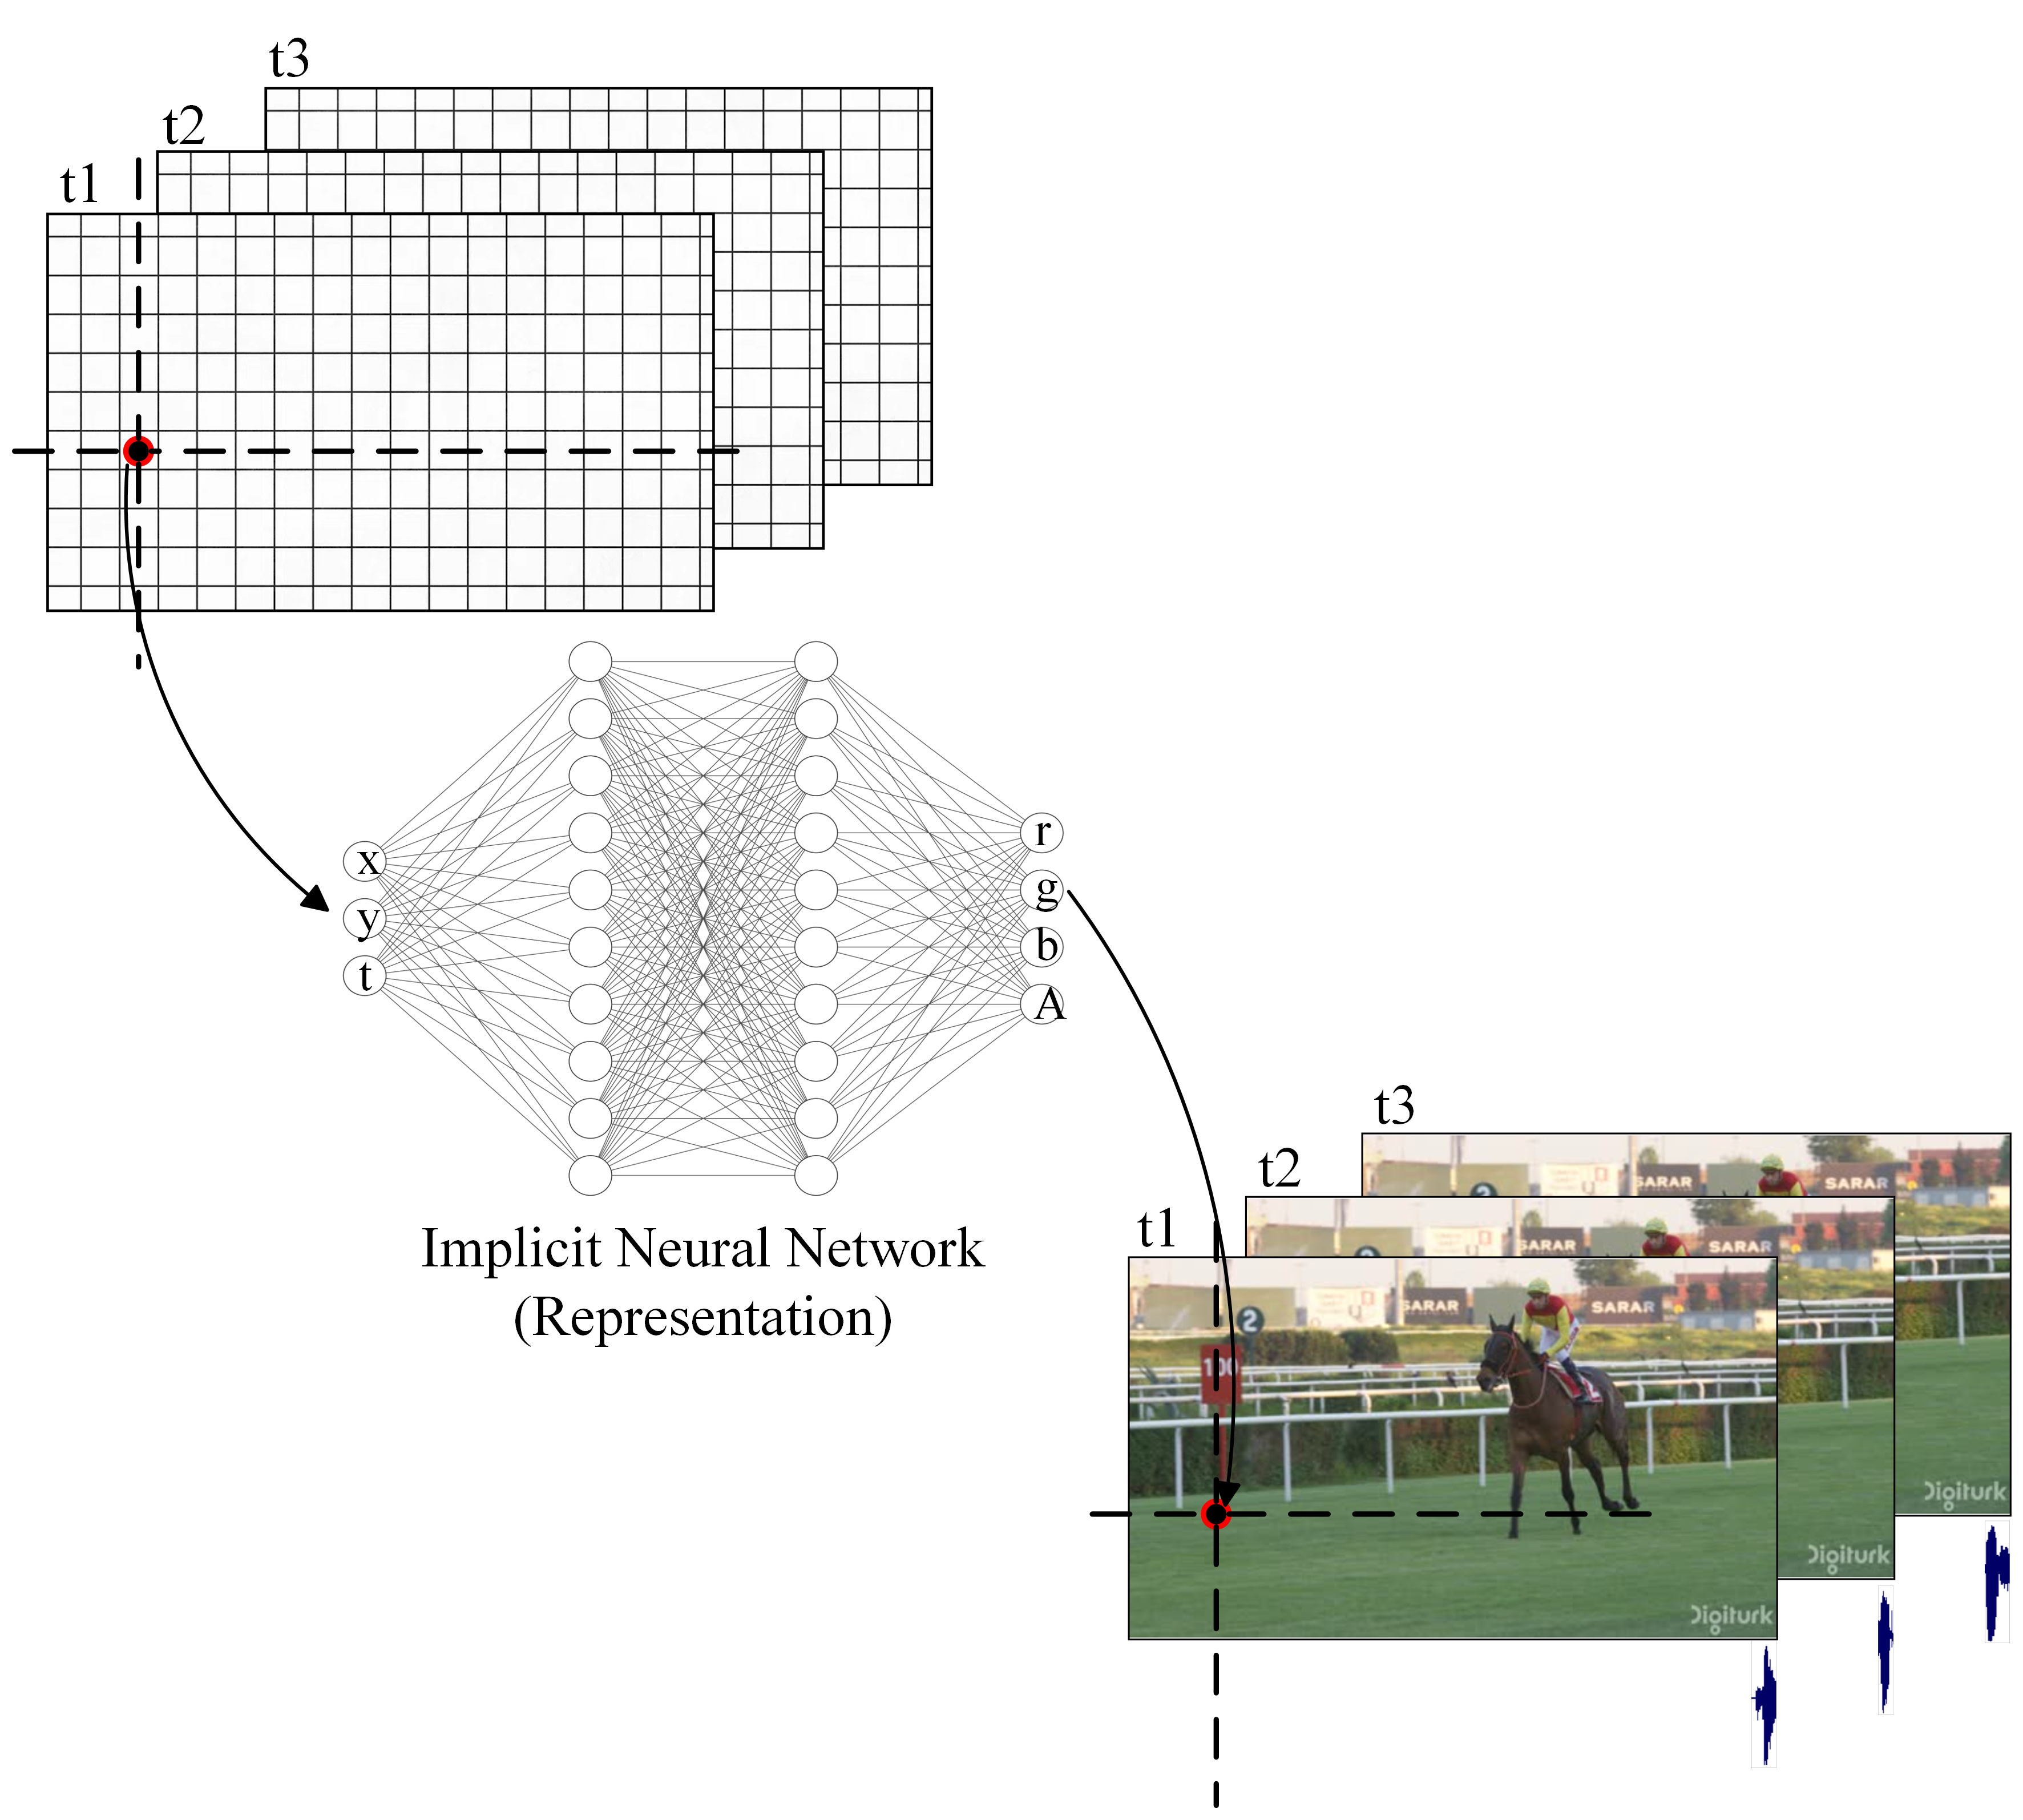
\includegraphics[height=0.45\textheight]{assets/INR.png}
        \caption{Representing Video in Neural Network}
        \label{fig:inr}
    \end{figure}
    \autoref{fig:inr} illustrates an Implicit Neural Representation (INR) where pixel coordinates $(x, y)$ and time index $t$ of video frames are fed into a neural network to output corresponding RGB values for visual data and amplitude for audio data. Sequential video frames $(t1, t2, t3)$ are divided into a grid of pixels. Each pixel's coordinates and time index are inputs to the network, which processes these inputs through several hidden layers. The network outputs the RGB values $(r, g, b)$ for each pixel's color and the amplitude $A$ for the associated audio. The outputs are then used to reconstruct the video frames and audio, demonstrating how the neural network encodes and decodes complex visual and audio information efficiently.
    \subsection{Fundamentals of INNs}
    \gls{inn} parameterize an unknown function \( f: \mathbb{R}^d \rightarrow \mathbb{R}^m \) where \( d \) and \( m \) represent the dimensions of the input and output spaces, respectively. This parameterization often involves a coordinate-based \gls{mlp} where the input coordinates are fed directly into the network, and the output is the function value at those coordinates. The network is trained using a loss function that minimizes the difference between the predicted and true function values over a set of sampled points.

    \subsection{Differences in Implicit Neural Network over Traditional Neural Network}

    \begin{figure}[H]
        \centering
        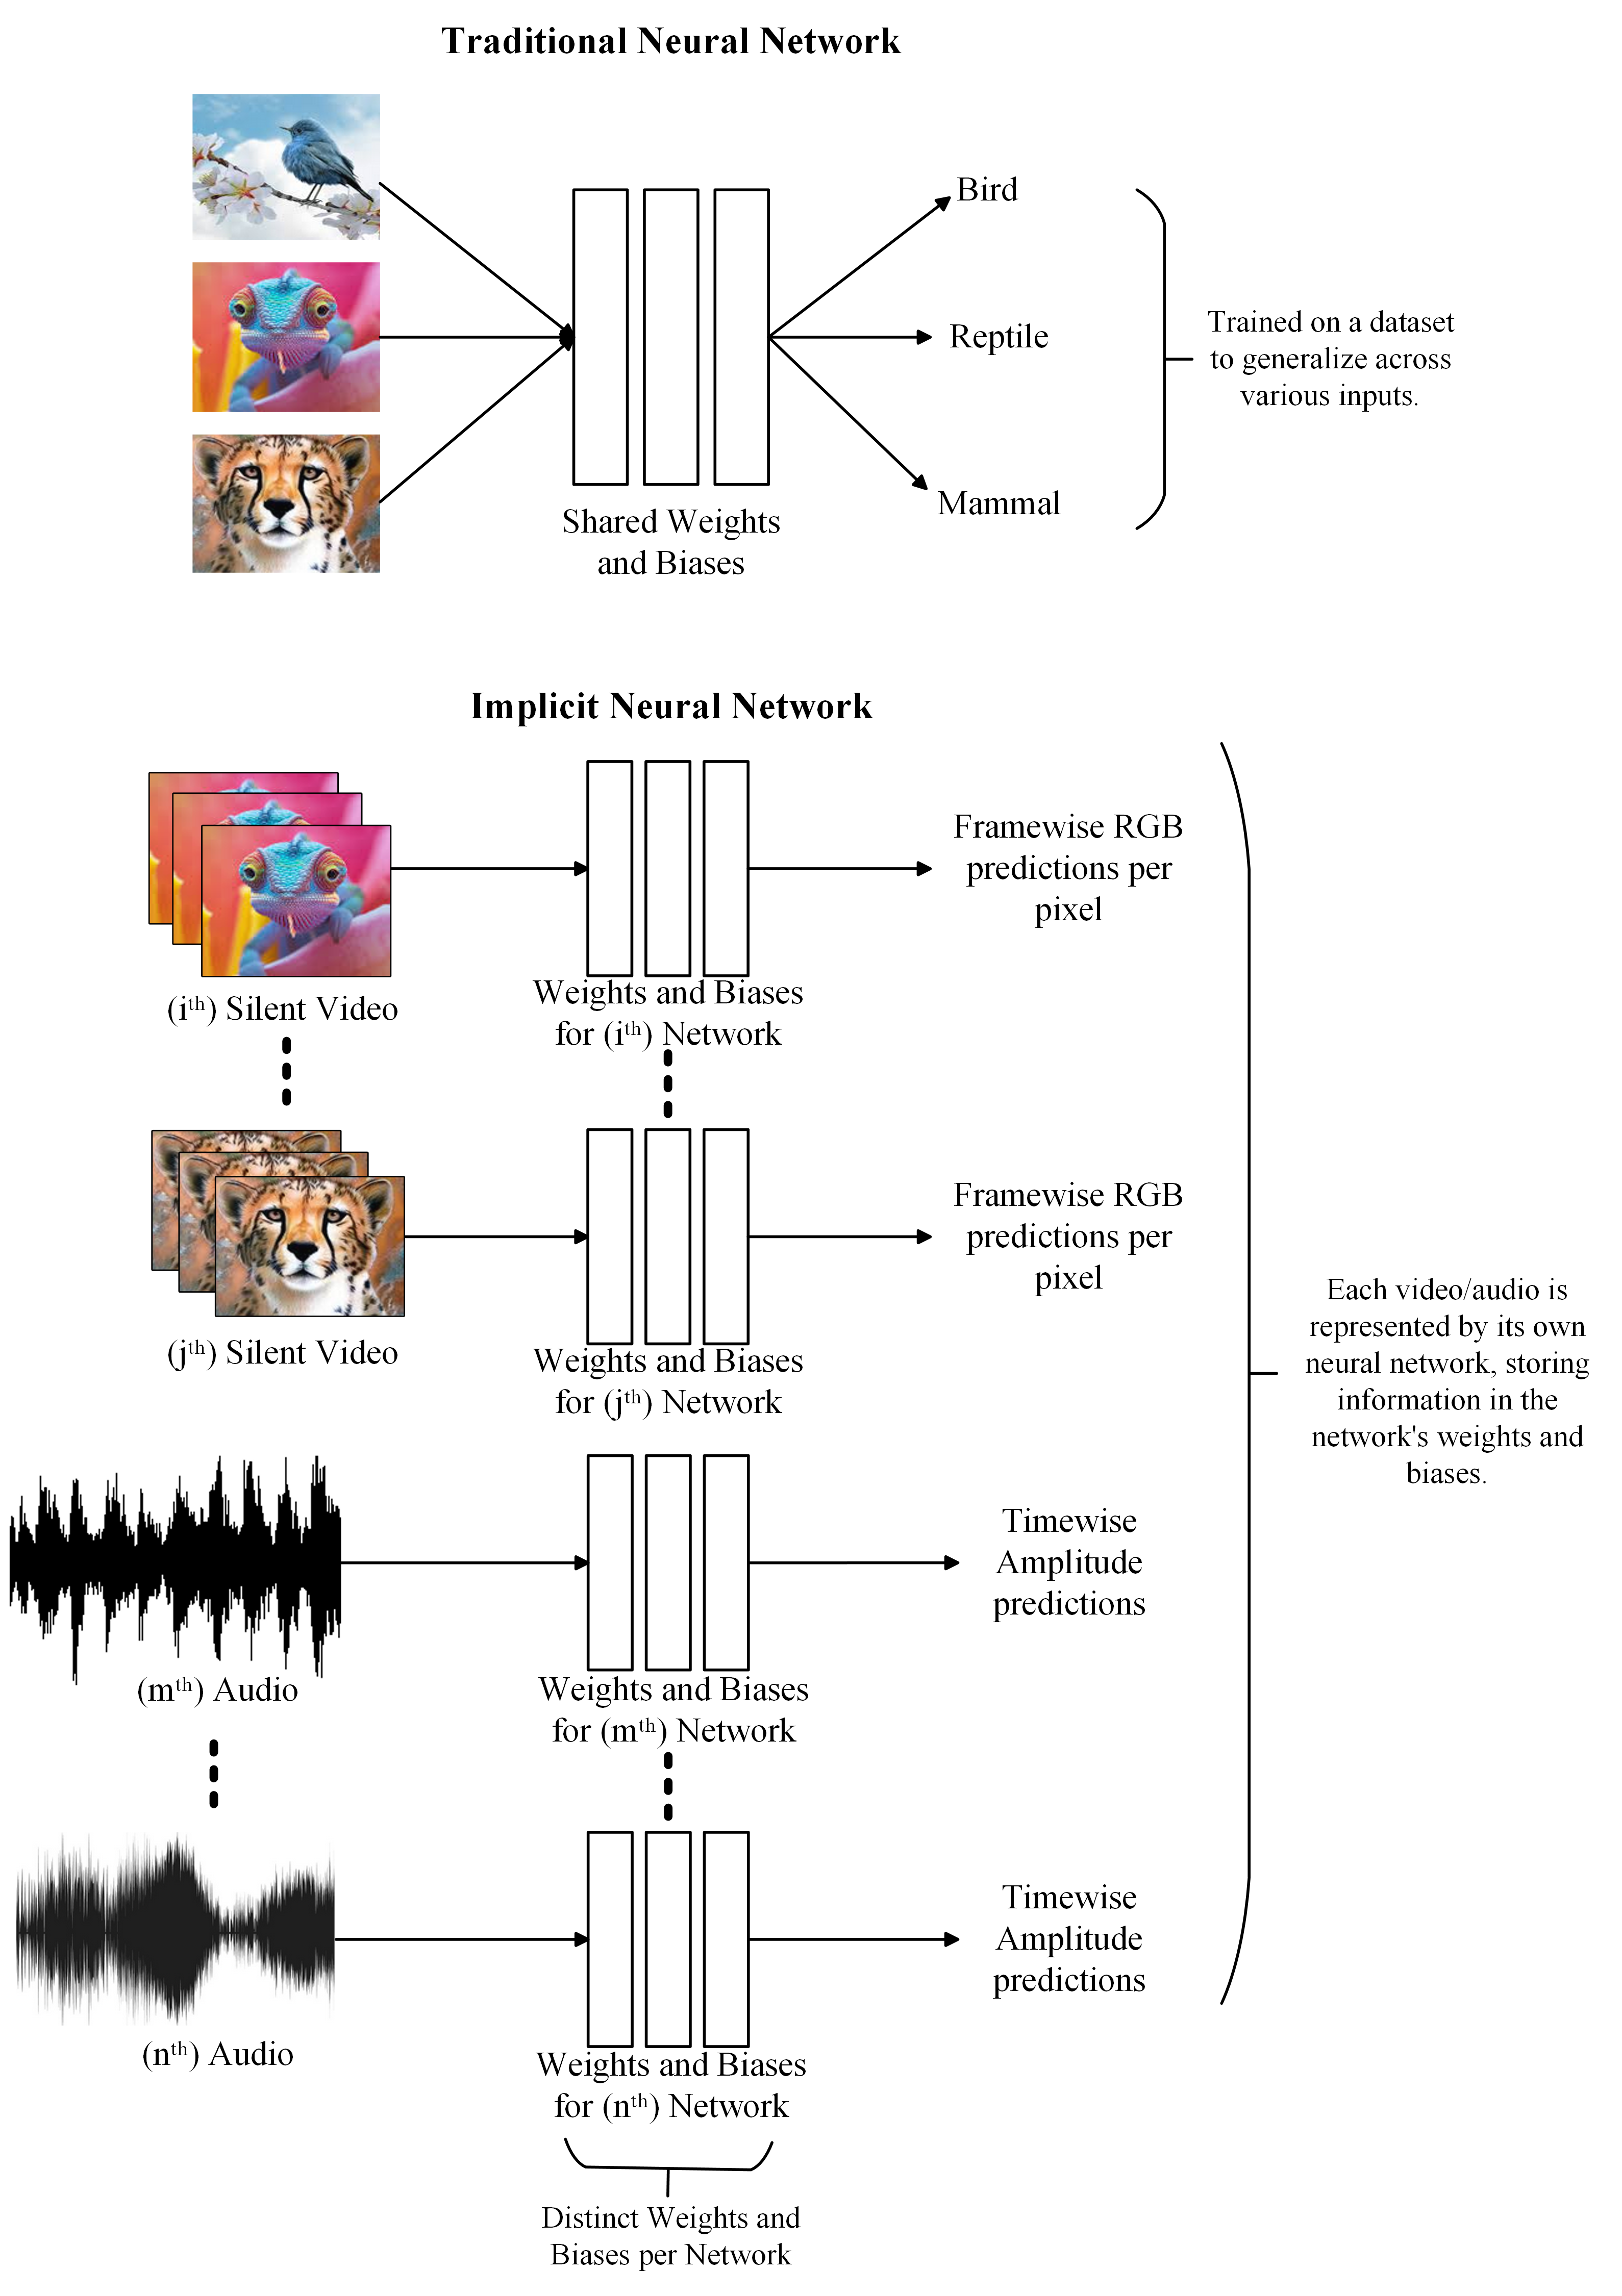
\includegraphics[width=0.95\linewidth]{assets/why overfitting.png}
        \caption{Implicit Neural Network vs Traditional Neural Network}
        \label{fig:implicit-vs-traditional}
    \end{figure}

    The \autoref{fig:implicit-vs-traditional} provides a visual comparison between traditional neural networks and implicit neural networks like SIREN (Sinusoidal Representation Network). Traditional neural networks utilize a single set of shared weights and biases for all inputs, aiming to generalize across a dataset. This generalization allows the network to accurately classify or predict outcomes for new, unseen data based on its training. For instance, in the \autoref{fig:implicit-vs-traditional}, a traditional neural network trained on images of birds, reptiles, and mammals uses the same network architecture to classify any new image into these categories.

    In contrast, implicit neural networks represent each piece of media with its own unique neural network, characterized by distinct weights and biases. This approach fundamentally changes the way these networks operate. Overfitting, typically seen as a drawback in traditional neural networks, becomes a beneficial feature in implicit neural networks. Overfitting allows the network to memorize and accurately reproduce the intricate details and nuances of the specific piece of media it represents. For example, in the image, each silent video and audio clip has its own dedicated neural network that predicts frame-wise RGB values per pixel or time-wise amplitude values, respectively.

    The advantages of this approach are:

    \begin{itemize}
        \item \textbf{Detail Preservation:} The overfitting ensures that the network captures and reproduces fine-grained details of the media.
        \item \textbf{Per-Media Specialization:} Each piece of media is encoded into its unique network, allowing for highly specialized and optimized representations.
    \end{itemize}

    Thus implicit neural networks like \gls{siren} create unique networks for each media piece, leveraging overfitting to capture detailed representations. This allows implicit neural networks to store intricate details within their parameters, making overfitting a beneficial feature.
    
    
    \subsection{Significance of Sinusoidal activation functions over traditional ones}

    The choice of activation functions in neural networks significantly influences their ability to model and process different types of data. The sine function is particularly suited for handling continuous inputs such as audio and video due to its inherent properties. Its smooth and periodic nature allows for efficient representation of continuous variations typical in audio waves or video frames. The smoothness of both the sine function and its derivative, a cosine wave, ensures that the gradients are well-defined across the entire function domain as shown in \autoref{fig:sinwave}. This characteristic is crucial during the neural network training process, which relies heavily on gradient-based optimization methods. The continuity and differentiability of the sine wave facilitate stable and effective weight updates, leading to reliable convergence in learning tasks.

    \begin{figure}[H]
        \centering
        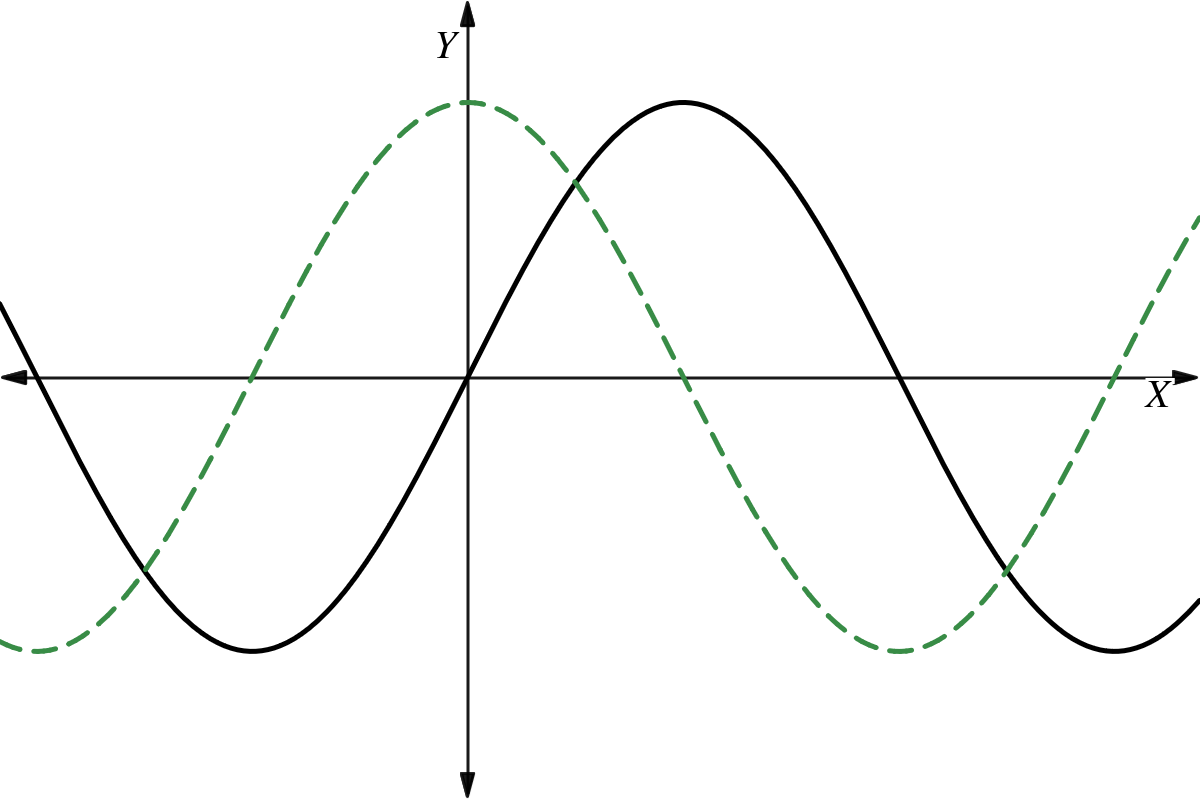
\includegraphics[height=0.25\textheight]{assets/sine-wave.png}
        \caption{Sine Wave and its Derivative}
        \label{fig:sinwave}
    \end{figure}

    In contrast, other waveforms like the triangular wave, although periodic, exhibit sharp transitions and corners at their peaks. The derivative of a triangular wave includes abrupt changes and discontinuities as we can see in \autoref{fig:triangular wave}, which can introduce complications in the learning process, particularly at points where the gradient becomes undefined. These discontinuities can potentially lead to instability in gradient calculations during backpropagation, adversely affecting the training efficiency and model performance. For neural networks involved in processing continuous data, such as in speech recognition or video processing, the sine function's ability to smoothly interpolate between values can capture complex, nuanced patterns more effectively. This smooth interpolation helps in better generalization and reduces the risk of overfitting to noisy variations, making the sine function a preferred choice for activation in networks dealing with continuous input signals.
    
    \begin{figure}[H]
        \centering
        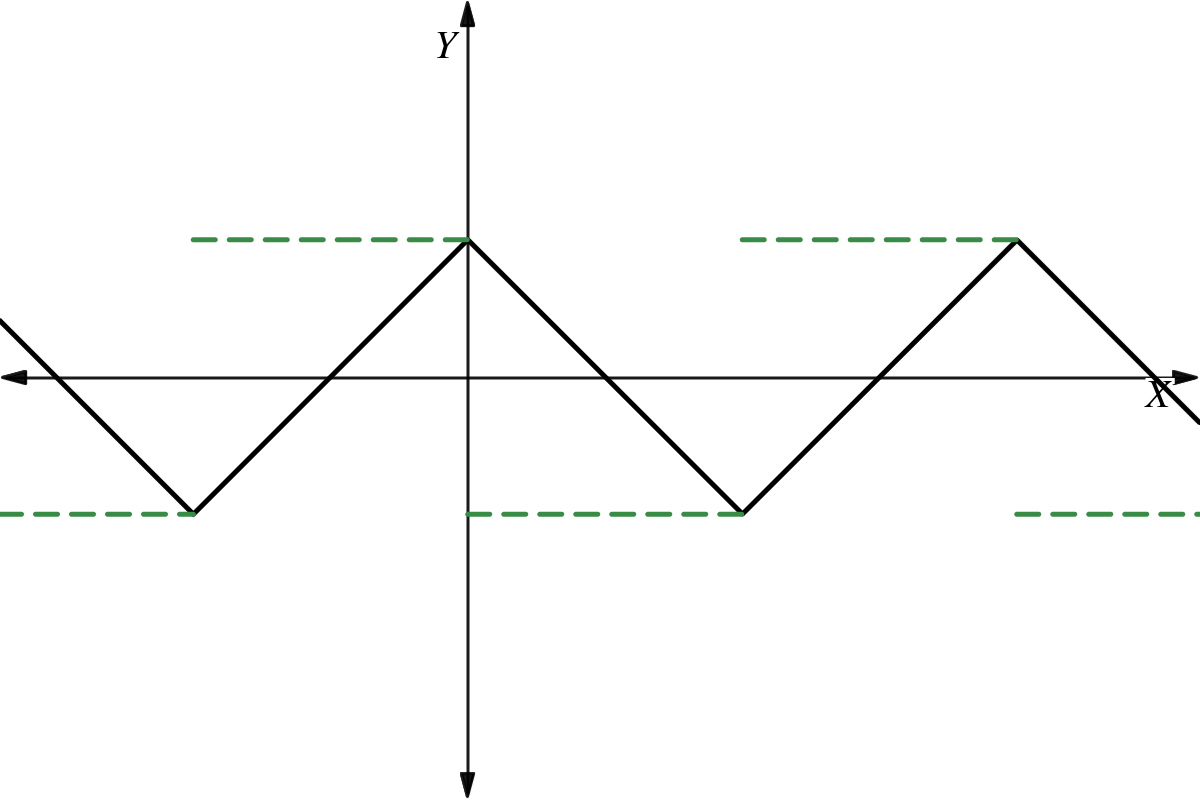
\includegraphics[height=0.25\textheight]{assets/triangular-wave.png}
        \caption{Triangular Wave and its Derivative}
        \label{fig:triangular wave}
    \end{figure}
    
    
    \begin{enumerate}[label=\textbf{\roman*.}]
        \item \textbf{Complex Signal Representation:} Sinusoidal activation functions enable neural networks to capture fine details and high-frequency components of signals more effectively. Traditional activation functions often struggle with this, leading to smoother, less detailed representations.
        \item \textbf{Smooth and Periodic Activation:} The smooth, continuous, and periodic nature of sinusoidal functions helps avoid issues like vanishing or exploding gradients, which are common with traditional activation functions, especially in deeper networks. This leads to more stable and efficient training dynamics.
        \item \textbf{Principled Initialization:} \gls{siren}s benefit from a principled initialization scheme tailored for sinusoidal activations, ensuring that the network starts with a configuration that is conducive to learning complex patterns without the instability seen with other activation functions.
    \end{enumerate}
    
    \subsection{Transition to Sinusoidal Representation Networks (SIRENs)}
    Building on the concept of \gls{inn}, \gls{siren} introduce a critical innovation by employing sinusoidal activation functions in all layers of the network. The general form of a \gls{siren} layer is expressed as:
    \begin{equation}
        x_{i+1} = \sin(W_i x_i + b_i)
    \end{equation}
    
    where \( x_{i+1} \) is the output of the \(i\)-th layer, serving as the input to the next layer, \( \sin \) is the sinusoidal activation function applied to each layer, \( W_i \) is the weight matrix of the \(i\)-th layer, \( x_i \) is the input to the \(i\)-th layer, and \( b_i \) is the bias vector of the \(i\)-th layer.
    
    \subsection{Initialization Scheme for Sinusoidal Representation Networks (SIRENs)}
    Sinusoidal Representation Networks uses the sine function as an activation, which introduces sensitivity to input distributions due to its periodic nature. An effective initialization scheme is crucial to prevent the degradation of the network's performance with increasing depth. This report proposes a principled approach to initialization that preserves the distribution of activations across layers, ensuring that the output at initialization does not vary with the number of layers.
    \subsubsection{Steps Involved in Initialization}
    \begin{enumerate}[label=\textbf{\roman*.}]
        \item \textbf{Initial Input and Single Neuron Output}
        \begin{itemize}
            \item Uniformly Distributed Input: The input $x$ is drawn from a uniform distribution $U(-1, 1)$, representing normalized coordinates used in applications such as image processing.
            \item Output of a Single Sine Neuron: The output of a neuron using the sine activation function is given by:
               \begin{equation}
                  y = \sin(ax + b) 
               \end{equation} 
            where $a$ and $b$ are the frequency and phase parameters, respectively. For $a > \frac{\pi}{2}$, ensuring at least half a period of the sine function, the output distribution $y$ is arcsine distributed over $[-1, 1]$.
        \end{itemize}
        \item \textbf{Layer-wise Propagation}
        \begin{itemize}
            \item Weights and Biases: Weights $w$ are initialized uniformly within $U\left(-\frac{c}{\sqrt{n}}, \frac{c}{\sqrt{n}}\right)$, where $c$ is a scaling factor and $n$ is the fan-in.
            \item Output of Deeper Layers: In subsequent layers, each input is arcsine distributed due to the previous layer's sine activation. The weighted sum $w^T x$ approaches a normal distribution as the number of inputs $n$ increases. Passing this sum through another sine function keeps the output arcsine distributed, preserving the distribution across layers.
        \end{itemize}
        \item \textbf{Special Handling in the First Layer} \\
          For the first layer, weights are adjusted by a factor $\omega_0$, set to 30. This adjustment ensures that the sine function: $\sin(\omega_0 \cdot Wx + b)$ spans multiple periods over the interval [-1, 1]. This extensive coverage is beneficial for handling the complex patterns and frequencies in video and audio data, enabling the network to capture a broad range of features initially.        
    \end{enumerate}

    \subsection{Knowledge Distillation for Model Compression}
    Knowledge distillation is a technique used in machine learning to transfer knowledge from a larger, more complex model (teacher) to a smaller, simpler model (student). This process aims to improve the efficiency and speed of the smaller model while maintaining or even enhancing its performance. One variant of knowledge distillation is \gls{rbkd}, which focuses on distilling knowledge related to the model's response or output behavior.

    The fundamental idea behind \gls{rbkd} is to train a student model to mimic not just the final predictions of the teacher model but also the intermediate responses or activations. This approach aims to capture the nuanced decision-making processes of the teacher model, enabling the student to generalize better and achieve comparable performance with fewer parameters.
    
    The main idea behind \gls{rbkd} revolves around the concept of feature representations and decision boundaries. By learning from the teacher model's response patterns, the student model can develop a deeper understanding of the underlying data distribution and make more informed predictions, especially in complex and high-dimensional input spaces.
    
    
    Soft Target Loss:
    The soft target loss remains the primary component in the distillation process. It compares the probabilities predicted by the student model to those of the teacher model:
    \begin{equation}
        L_{\text{soft}} = \text{CrossEntropy}(S(x), T(x))
    \end{equation}
    
    where $L_{\text{soft}}$ is the soft target loss, $S(x)$ is the student model's output, and $T(x)$ is the teacher model's output for input $x$.
    
    The overall loss function simplifies to just the soft target loss without the response matching component:
    \begin{equation}
        L_{\text{total}} = \alpha L_{\text{soft}}
    \end{equation}

    where  $L_{\text{total}}$ is the total loss function, $\alpha$ is a hyperparameter controlling the importance of the soft target loss, and $L_{\text{soft}}$ is the soft target loss as defined above.
    \begin{figure}[H]
        \centering
        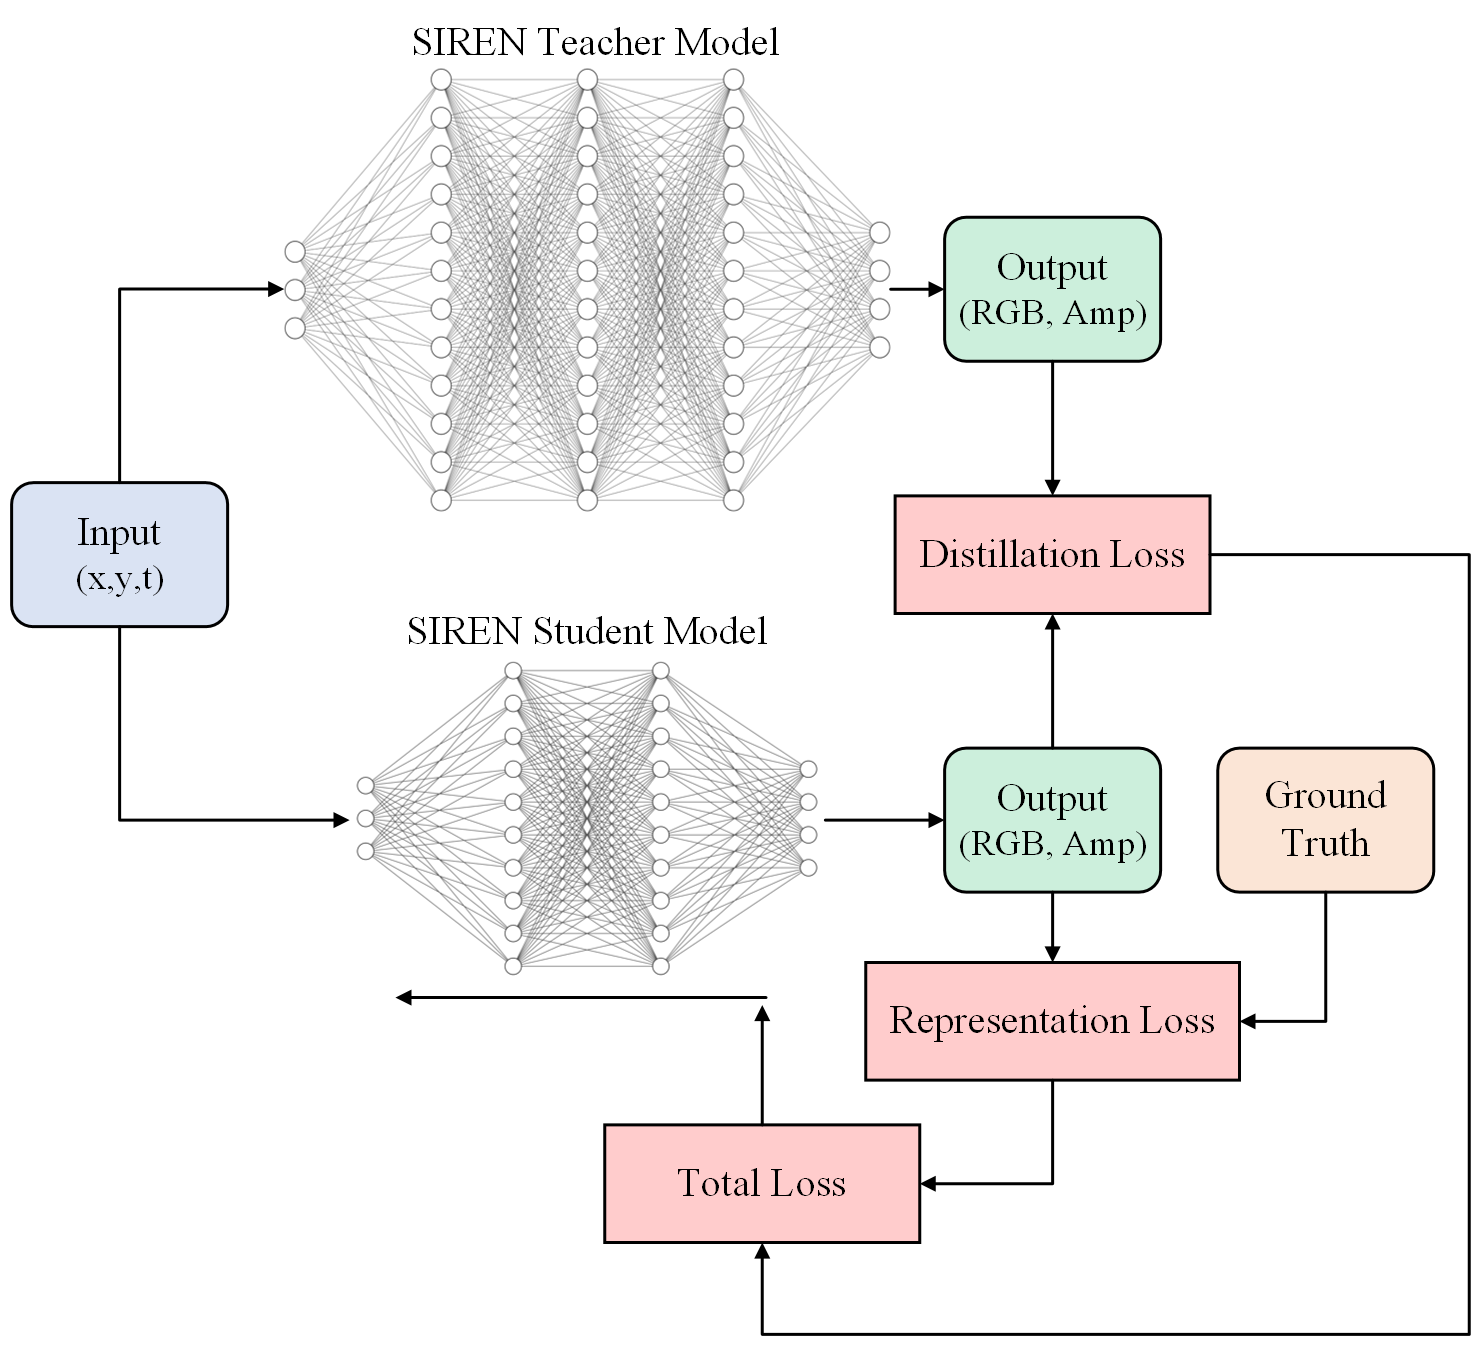
\includegraphics[width=0.95\linewidth]{assets/Knowledge Distillation.png}
        \caption{Block Diagram of Knowledge Distillation}
        \label{fig:block-diagram-knowledge-distillation}
    \end{figure}
    In \autoref{fig:block-diagram-knowledge-distillation}, the teacher model is a SIREN (Sinusoidal Representation Networks) network pretrained on audio-visual data, while the student model is a shallower version designed to learn from the teacher's responses.

    The inputs to both models are in the form of (x, y, t), where (x, y) represent spatial coordinates in the video, and t represents time. The teacher model outputs four values: r, g, b (RGB values corresponding to (x, y, t)), and Amplitude (corresponding audio amplitude for the given (x, y, t)). Notably, the (x, y) coordinates are ignored in the context of audio amplitude.
    
    During response-based knowledge distillation, the student model's predictions are compared against the teacher model's predictions. This comparison helps calculate the distillation loss, which captures the discrepancy between the student's output and the teacher's output. Simultaneously, the ground truth provides the representation loss, measuring how well the student model represents the actual data.
    
    These two types of losses, distillation loss and representation loss, are typically weighted and combined to calculate the total loss. This total loss is then used for feedback and backpropagation during the training process, allowing the student model to gradually learn and mimic the behavior of the more complex teacher model.
    
    By using response-based knowledge distillation, the student model can benefit from the rich representations learned by the teacher model, even though it has a simpler architecture. This approach is particularly useful for tasks where computational resources or model complexity are constrained, yet high performance is desired.

    \subsection{Pruning}
    Pruning is a technique used to reduce the size of a neural network by removing unnecessary or less important parameters (weights and neurons). Pruning reduces the complexity of the neural network by removing weights that have minimal impact on the model’s output, thereby reducing overfitting and improving the model's generalization capabilities.
    \begin{equation}
        W = W \cdot \mathbf{1}_{|W| > \theta}
    \end{equation}
    where \( W \) is the weight matrix, \( \theta \) is a threshold for pruning, and \( \mathbf{1} \) is the indicator function.

    \begin{figure}[H]
            \centering
            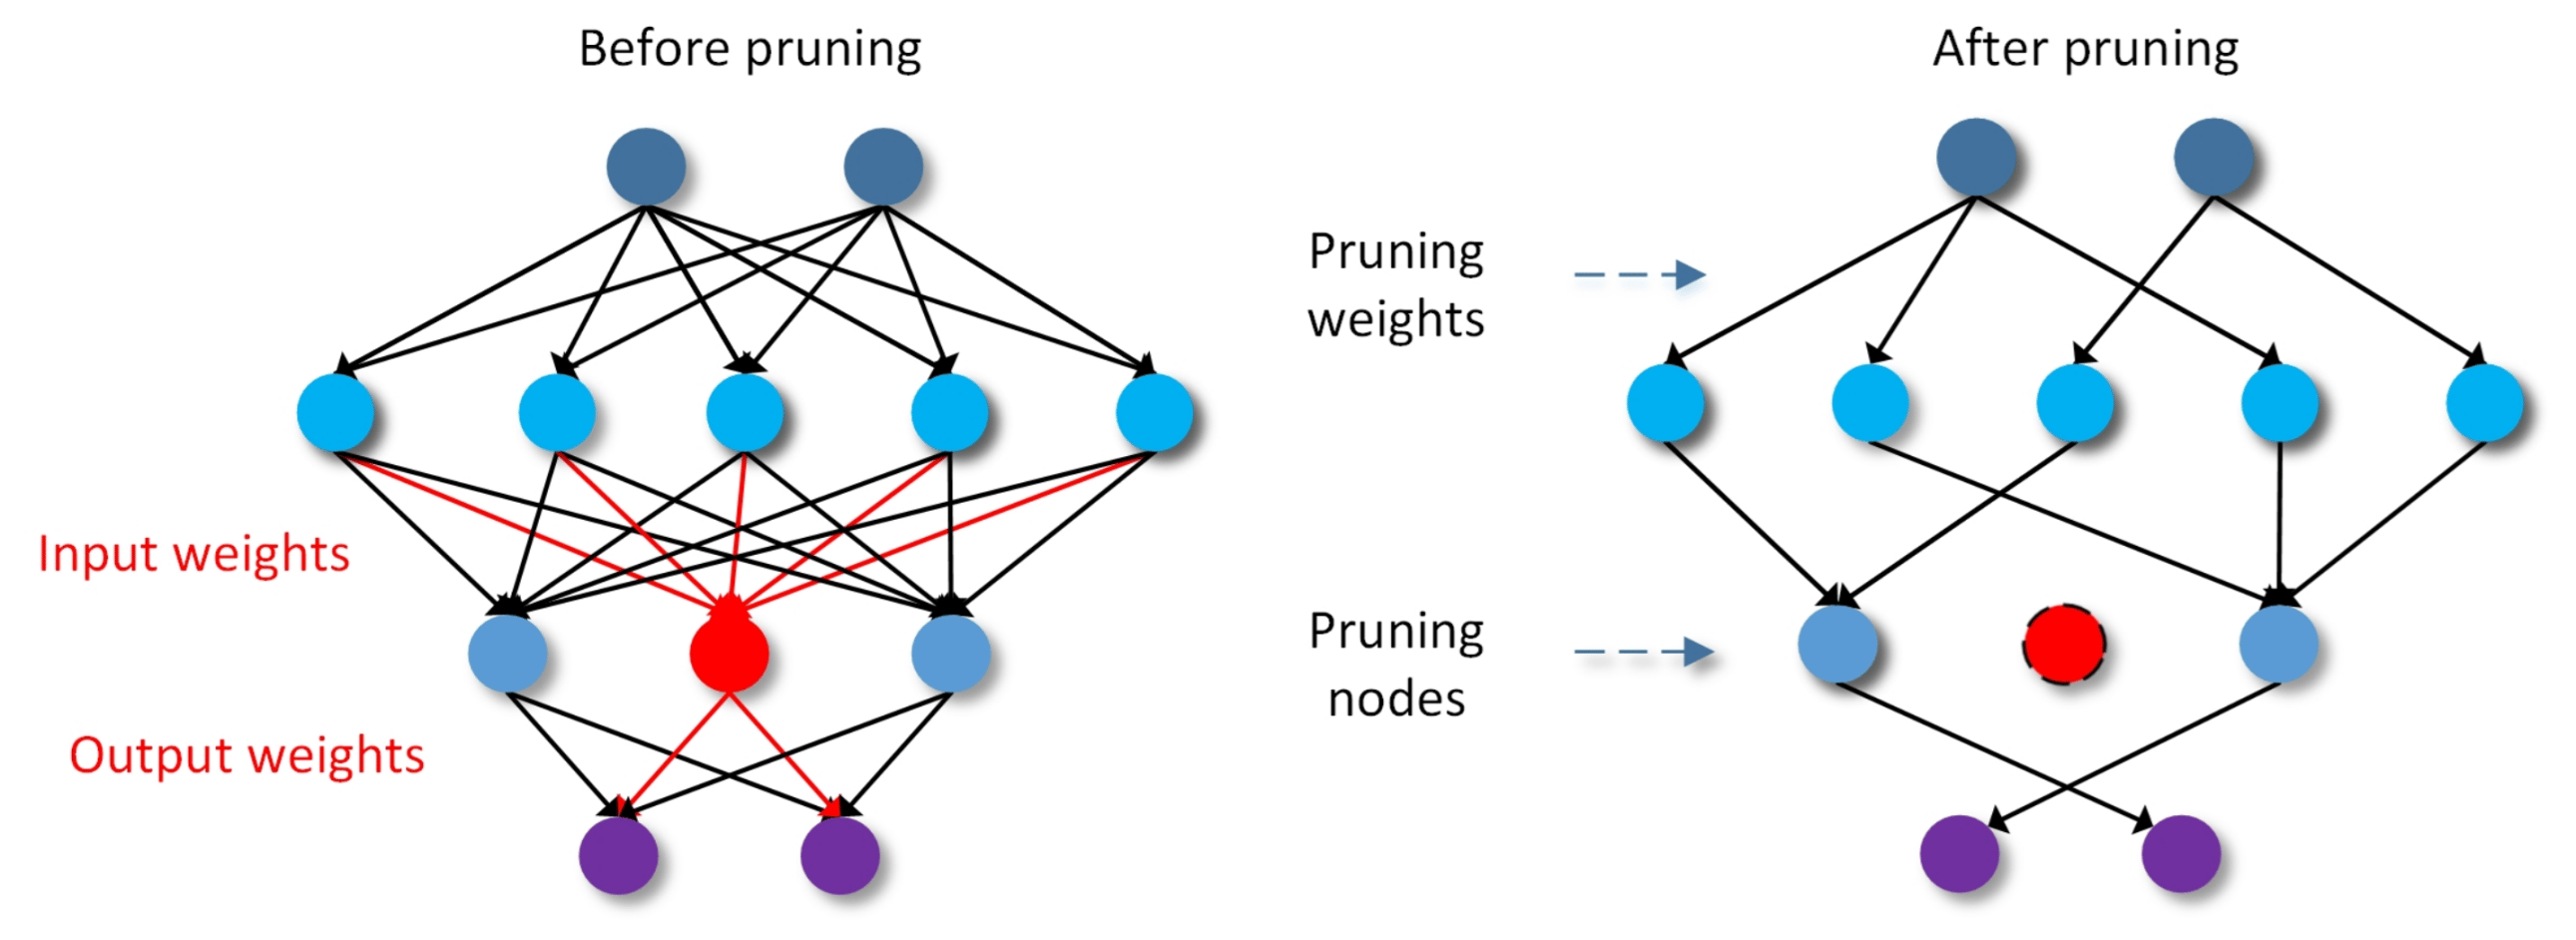
\includegraphics[width=\linewidth]{assets/conceptual figure of pruning.png}
            \caption{Pruning}
            \label{fig:conceptual-pruning}
    \end{figure}
    \autoref{fig:conceptual-pruning} shows network pruning which involves selectively removing weights from fully connected layers that fall below a specified threshold, to reduce model complexity. Additionally, unnecessary nodes are eliminated to optimize computational efficiency and enhance model performance.
    
    \subsection{Quantization}
    Quantization involves reducing the precision of the model's parameters, such as weights, from floating-point to lower-bit representations, which decrease the model size.
    \begin{equation}
        w' = \text{round}\left(\frac{w}{s}\right)
    \end{equation}
    where \( w \) is the original weight, \( s \) is a scaling factor, and \( w' \) is the quantized weight.

    \begin{figure}[H]
            \centering
            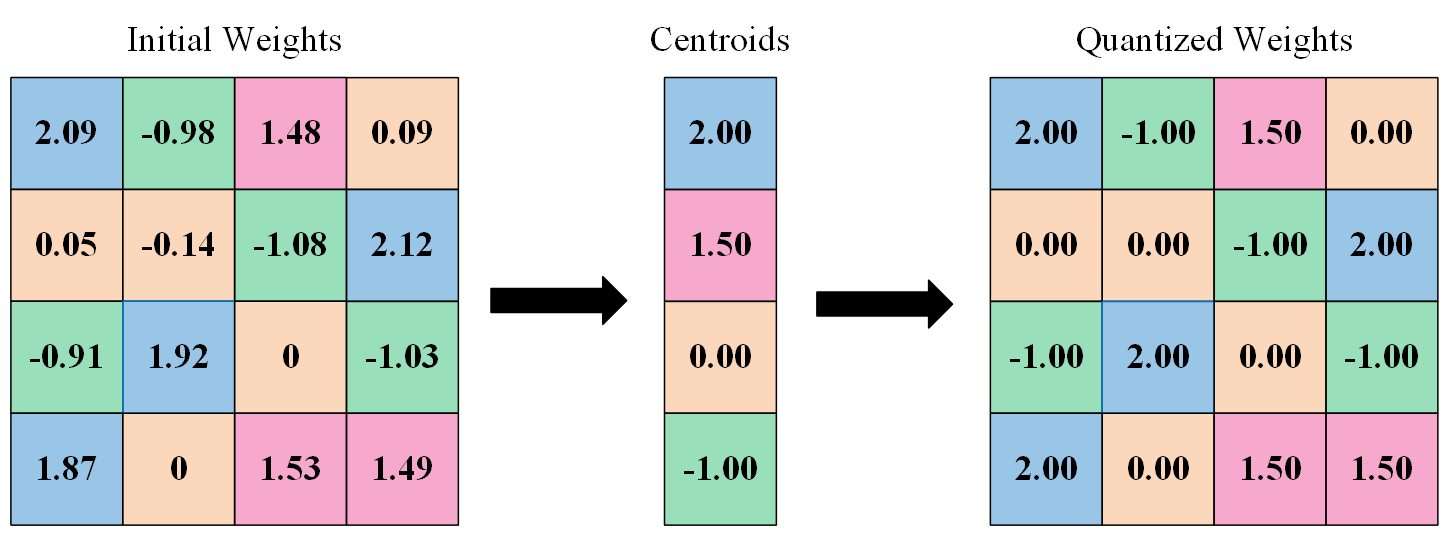
\includegraphics[width=\linewidth]{assets/conceptual figure of quantization.png}
            \caption{Quantization}
            \label{fig:conceptual-quantization}
    \end{figure}
    In \autoref{fig:conceptual-quantization}, a sample 4x4 matrix of weights is taken. The weights are quantized to 4 bins (denoted with 4 colors),
    all the weights in the same bin share the same value. The centriods for each bin can be found using K-Means Clustering. For updating the centriods, the gradients  are grouped according to the bins, summed together, multiplied by the learning weight and subtracted from the previous centriod. The weights are then replaced by the centroids of the respective bins.
        
    \subsection{Variational Autoencoder (VAE) }
        \begin{figure}[H]
        \centering
        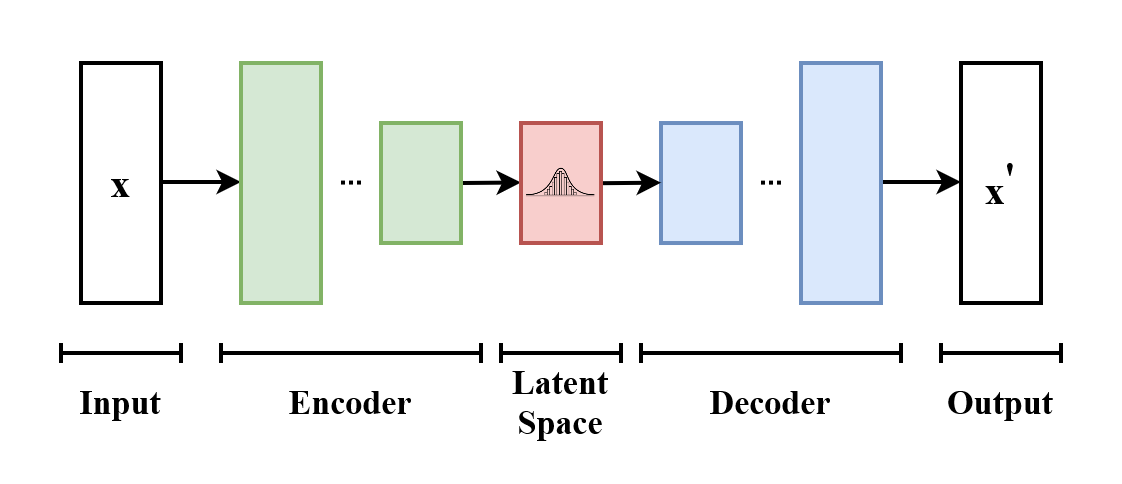
\includegraphics[width=0.95\linewidth]{assets/VAE_Basic.png}
        \caption{Variational Autoencoder}
        \label{fig:vae}
    \end{figure}
    \autoref{fig:vae} illustrates the architecture and workflow of a Variational Autoencoder (VAE), capturing the process from input to output through a series of transformations within the encoder, latent space, and decoder. The input, denoted as $\mathbf{x}$, represents the neural network parameters (weights and biases). These parameters are flattened and normalized into a high-dimensional vector. The goal is to transform these parameters into a manageable, lower-dimensional latent representation while retaining essential performance characteristics. The encoder processes the input data $\mathbf{x}$ and maps it into the latent space. Unlike traditional autoencoders, the VAE encoder outputs parameters defining Gaussian distributions for each latent dimension: mean $\mu$ and variance $\sigma^2$. The equations governing this transformation are:
    \begin{equation}
           \mu = f_{\mu}(\mathbf{x}), \quad \sigma^2 = f_{\sigma}(\mathbf{x})
    \end{equation}

    where $f_{\mu}$ and $f_{\sigma}$ are functions modeled by the neural network.

    Each set of model parameters is represented as a distribution in the latent space, rather than a single point. The reparametrization trick allows sampling from these distributions while maintaining differentiability, crucial for backpropagation. The latent variable $\mathbf{z}$ is sampled as follows:
    \begin{equation}
    \mathbf{z} = \mu + \sigma \cdot \epsilon, \quad \epsilon \sim \mathcal{N}(0, I)
    \end{equation}
    where $\epsilon$ is a random variable sampled from a standard normal distribution.

    The decoder takes the latent variable $\mathbf{z}$ and reconstructs the model parameters $\mathbf{x'}$. The aim is to invert the encoding process, mapping $\mathbf{z}$ back to the original parameter space. The quality of reconstruction is measured by the similarity between $\mathbf{x'}$ and $\mathbf{x}$, impacting the model's performance.

    The output $\mathbf{x'}$ is the reconstructed version of the model parameters. The loss function used to train the VAE includes the reconstruction loss and the Kullback-Leibler (KL) divergence:
    \begin{equation}
    \mathcal{L} = \|\mathbf{x} - \mathbf{x'}\|^2 + D_{KL}(q(\mathbf{z}|\mathbf{x}) \| p(\mathbf{z}))
    \end{equation}
    where $D_{KL}$ denotes the KL divergence, promoting effective learning of the latent space distribution.

\pagebreak



\section{\MakeUppercase{Mathematical Formulation}}

\subsection{Mathematical Modeling in SIRENs}
\gls{siren} excel in tasks requiring the modeling of periodic and smooth phenomena, which are common in audio and video signals. The continuous nature of the function modeled by \gls{siren} makes them ideal for compressing these signals efficiently. The typical loss function used for training \gls{siren} in the context of compression is the \gls{mse}, which ensures the fidelity of the reconstructed signal:
\begin{equation}
    L = \frac{1}{N} \sum_{n=1}^N (\Phi(\mathbf{x}_n) - y_n)^2 
\end{equation}
Additionally, to capture temporal dynamics in video and audio, derivatives of the function are often included in the training objective:
\begin{equation}
    L = \frac{1}{N} \sum_{n=1}^N \left((\Phi(\mathbf{x}_n) - y_n)^2 + \lambda (\nabla\Phi(\mathbf{x}_n) - \nabla y_n)^2\right) 
\end{equation}
where \( N \) is the total number of sampled points, \( \Phi \) is the SIREN model, \( \mathbf{x}_n \) are the input coordinates for the \(n\)-th data point, \( y_n \) are the actual output values at the \(n\)-th data point, \( \lambda \) is a regularization parameter, \( \nabla\Phi(\mathbf{x}_n) \) is the derivative of the \gls{siren} output with respect to the input at \( \mathbf{x}_n \), and \( \nabla y_n \) is the derivative of the true output values with respect to the input at \( \mathbf{x}_n \).


\subsection{\MakeUppercase{Forward and Backward propagation in SIREN network}}
\begin{figure}[H]
    \centering
    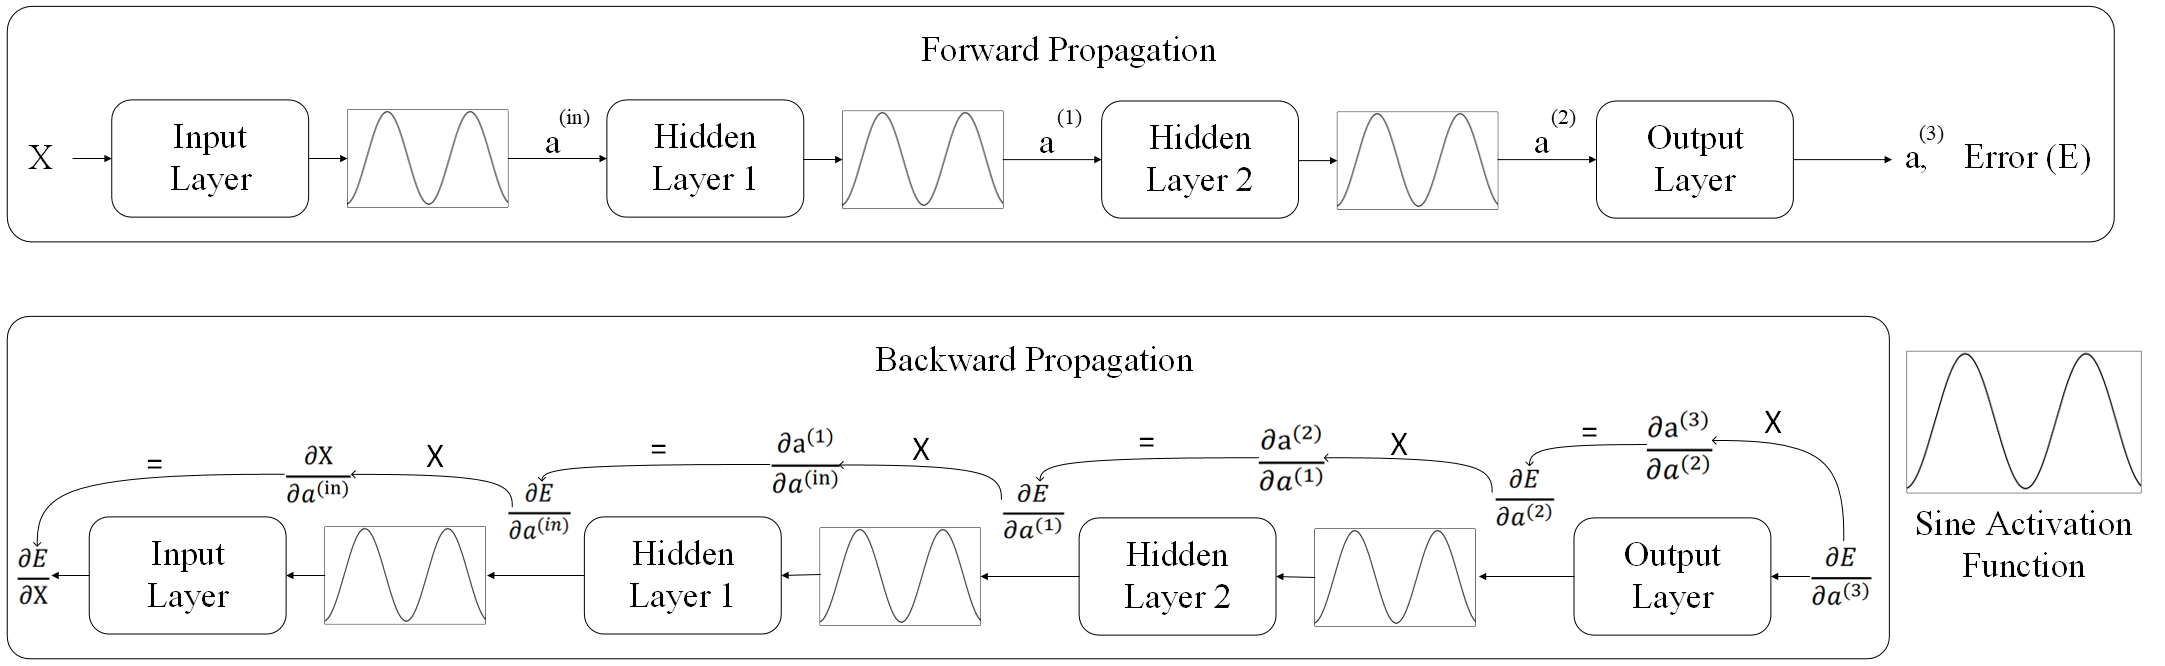
\includegraphics[width=\linewidth]{assets/Propagation concept figure Major Project.png}
    \caption{Forward and Backward Propopagation in SIREN network}
    \label{fig:propagation-diagram}
\end{figure}

The figure provides a illustration of the forward and backward propagation processes in a siren neural network. In the forward propagation section, the input \( \mathbf{X} \) is passed through the input layer, then sequentially through hidden layers 1 and 2, and finally through the output layer to compute the activations \( \mathbf{a}^{(1)} \), \( \mathbf{a}^{(2)} \), and \( \mathbf{a}^{(3)} \). The error \( \mathbf{E} \) is calculated based on the difference between the predicted output \( \mathbf{a}^{(3)} \) and the actual output \( \mathbf{y}_i \). 

The backward propagation section shows the gradient calculation needed to update the network's weights. It starts with the error gradient \( \frac{\partial \mathbf{E}}{\partial \mathbf{a}^{(3)}} \) at the output layer and propagates backwards through hidden layers 2 and 1, and finally to the input layer. This involves computing the gradients \( \frac{\partial \mathbf{a}^{(3)}}{\partial \mathbf{a}^{(2)}} \), \( \frac{\partial \mathbf{a}^{(2)}}{\partial \mathbf{a}^{(1)}} \), and \( \frac{\partial \mathbf{a}^{(1)}}{\partial \mathbf{a}_{(in)}} \).
The weights and biases are updated as per the following equations:
\begin{equation}
    W^{(l)} \leftarrow W^{(l)} - \eta \frac{\partial E}{\partial W^{(l)}}  
\end{equation}
\begin{equation}
    b^{(l)} \leftarrow b^{(l)} - \eta \frac{\partial E}{\partial b^{(l)}}  
\end{equation}



Where:
\begin{itemize}
    \item \( W^{(l)} \) represents the weights of the \( l \)-th layer.
    \item \( b^{(l)} \) represents the weights of the \( l \)-th layer.
    \item \( \eta \) is the learning rate.
    \item \( \frac{\partial E}{\partial W^{(l)}} \) is the gradient of the error with respect to the weights of the \( l \)-th layer.
    \item \( \frac{\partial E}{\partial b^{(l)}} \) is the gradient of the error with respect to the biases of the \( l \)-th layer.
\end{itemize}
The detailed forward and backward propagation equations and the gradients of error with respect to weight and bias matrices are provided in \autoref{app:forward-backward-eqn}



\subsection{KL Divergence and Earth Mover's Distance}

\subsubsection{KL Divergence}
\gls{kld} is a measure of how one probability distribution diverges from a second, expected probability distribution. It quantifies the difference between two distributions \( P \) and \( Q \).

\begin{equation}
    D_{KL}(P \parallel Q) = \sum_{i} P(i) \log \frac{P(i)}{Q(i)}
\end{equation}

\subsubsection{Earth Mover's Distance (EMD)}
\gls{emd} is a measure of the distance between two probability distributions over a region \( D \). It is the minimum cost to transform one distribution into the other, viewed as the "work" needed to move the distribution mass.

\begin{equation}
    \text{EMD}(P, Q) = \inf_{\gamma \in \Gamma(P,Q)} \int_{D \times D} d(x, y) \, d\gamma(x, y)
\end{equation}

where \( \Gamma(P, Q) \) is the set of all possible joint distributions whose marginals are \( P \) and \( Q \), and \( d(x, y) \) is the ground distance between elements \( x \) and \( y \).

\pagebreak

\section{\MakeUppercase{System Architecture and Methodology}}   
This section provides an overview of the system architecture and the methodology used in video \gls{codec} with a implicit neural network-based approach.
    \subsection{Block Diagram}
        \begin{figure}[H]
            \centering
            \includegraphics[width=\linewidth]{assets/Major Block Diagram.png}
            \caption{System Block Diagram}
            \label{fig:Block-Diagram}
        \end{figure}
        
        \autoref{fig:Block-Diagram} outlines a comprehensive process for encoding and decoding video with audio using an advanced neural network-based approach. Initially, frames and corresponding audio are extracted from the input video. These elements are then converted into a space-time coordinate system, integrating both the spatial dimensions of the video and the temporal aspects of both video and audio. This data feeds into a fully connected neural network model, trained to predict the \gls{rgb} values for each pixel and the amplitude for the audio at each time step. Post-training, the model undergoes compression through knowledge distillation. The output from the student model is a compressed version of the original video and audio, ready for transmission. The compressed model can then be stored or transmitted. The compressed model will be used to reconstruct the video and audio by sampling the model using the space-time coordinates. The reconstructed outputs are concatenated to produce the final video with audio output, matching the original input in content and synchronization.

        \subsubsection{Input Video with Audio}
        The process begins with an input video that includes both visual and auditory information, serving as the source material for the subsequent encoding and compression processes.

        \subsubsection{Frame and Audio Extraction}
            \begin{itemize}
              \item \textbf{Frame Extraction:} Video is separated into individual frames, each representing a snapshot of the visual content at a specific point in time.
              \item \textbf{Audio Extraction:} The audio track is extracted concurrently, maintaining synchronization with the video frames to ensure each frame correlates with a precise segment of the audio.
                \end{itemize}
    
        \subsubsection{Space-Time Coordinate Mapping}
        Each pixel in a frame is assigned coordinates $(x, y, t)$, where $x$ and $y$ represent the pixel's location within the frame, and $t$ represents the time, correlating with both the frame number and the corresponding audio segment.
        
        \subsubsection{Training Model (Fully Connected Neural Network)}
        A specially designed neural network consisting of multiple fully connected layers is trained to accept space-time coordinates as input and output the corresponding \gls{rgb} values for pixels and the amplitude for the audio, effectively mapping these inputs to their visual and auditory outputs.
    
        \subsubsection{Compression Pipeline}
        \begin{enumerate}[label=\textbf{\roman*.}]
          \item \textbf{Teacher Model:} This is a pre-trained or more complex model that captures comprehensive details and intricacies of the video and audio data.
          \item \textbf{Knowledge Distillation:} Information and learned patterns from the teacher model are transferred to a simpler, more efficient student model. This process involves training the student model to mimic the output of the teacher model but with less computational overhead or more optimized for specific tasks like compression.
          \item \textbf{Student Model:} A simplified version of the teacher model that is optimized for operational efficiency. This model is used for the actual compression, utilizing the distilled knowledge to maintain quality while reducing file size. The output from the student model is a compressed version of the original video and audio, ready for transmission.
          
        \item \textbf{Model Pruning:} Redundant parameters within the network are removed post- overfitting to streamline the model without significantly affecting its output accu- racy.
        \item \textbf{Model Quantization:} The network parameters are reduced in precision, which decreases the model size but retains essential information.
        \item \textbf{Model Encoding:} The encoding process is conducted using a \gls{vae}. In this process, the quantized model weights are input into the \gls{vae}, which then transforms these quantized weights into a compact representation within the latent space
    
        \end{enumerate}

        \subsection{Model Decoding}
        The decoding process is facilitated through the use of a \gls{vae}. During this phase, the latent representations, previously encoded, are input back into the \gls{vae}. The decoder then reconstructs the quantized model weights from these latent variables, effectively translating the compressed data back into its original, functional form.
        \subsubsection{Reconstruction}
        \begin{enumerate}[label=\textbf{\roman*.}]
          \item \textbf{Pixel-wise Output Generation:} Space-time coordinates are processed using the compressed model to regenerate \gls{rgb} values for each pixel and amplitude values for the audio at each time step.
          \item \textbf{Concatenation:} Individual outputs are concatenated to reconstruct the frames and audio track, reassembling the video and audio into a coherent output.
        \end{enumerate}
        
        \subsubsection{Reconstructed Video with Audio}
        The final output is a fully reconstructed video with audio that has been compressed, encoded, and then decoded, demonstrating the effectiveness of the neural network in handling complex video and audio data processing tasks.
    
    \subsection{Pre-processing Pipeline}
    \begin{figure}[H]
        \centering
        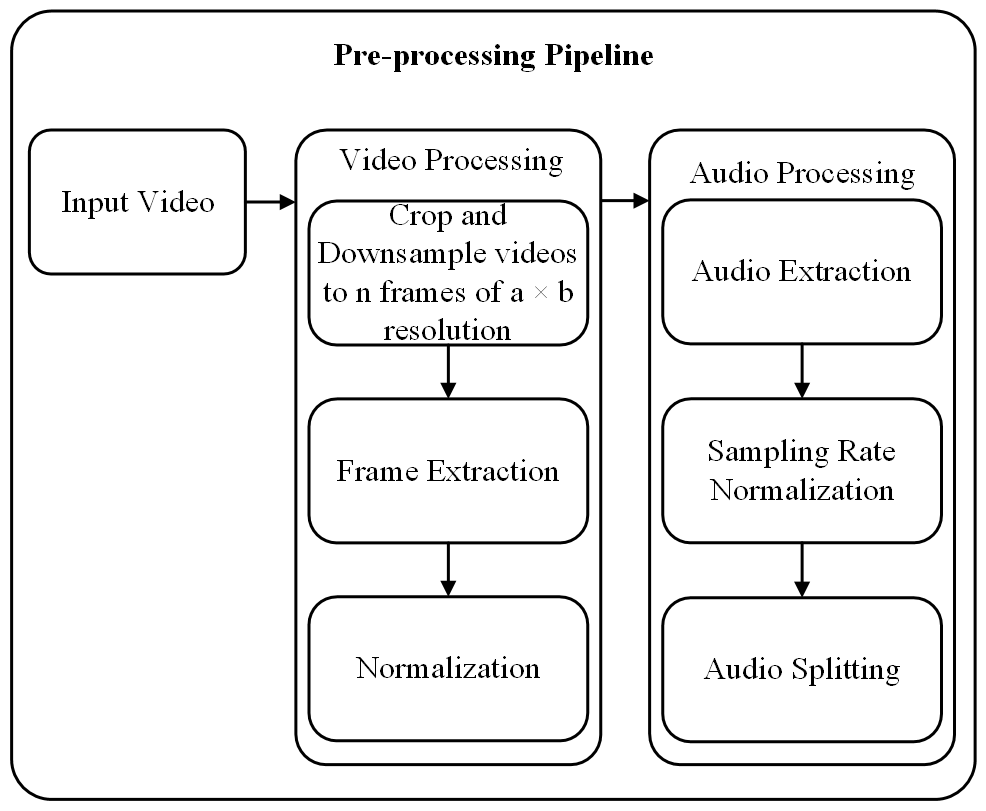
\includegraphics[width=0.9\linewidth]{assets/Major Data Pre-Processing.png}
        \caption{Pre-processing Pipeline}
        \label{fig:pre-processing-pipeline}
    \end{figure}
    
    \subsubsection{Overview of Pre-processing Pipeline for Video with Audio}
    \autoref{fig:pre-processing-pipeline} illustrates a pre-processing pipeline designed for handling video files with accompanying audio tracks. The pipeline is organized into two main branches for processing video and audio data, respectively. Each branch standardizes and optimizes the data for further analysis or processing.
    
    \subsubsection{Video Processing Branch}
    \begin{enumerate}[label=\textbf{\roman*.}]
        \item \textbf{Crop and Downsample Videos:}
        The initial step adjusts the resolution and frame dimensions of the video to a uniform size (\(a \times b\)) and reduces the number of frames to a standard count (`n'). This standardization is crucial for ensuring that subsequent processing stages operate on consistent and manageable data sizes.
        
        \item \textbf{Frame Extraction:}
        The processed video is then decomposed into individual frames. This conversion of the video into a sequence of images allows for the application of image processing techniques and facilitates detailed frame-by-frame analysis.
        
        \item \textbf{Normalization:}
        Pixel values of each frame are normalized to scale the intensity values typically to a range between 0 and 1. Normalization is a critical step for preparing data for many types of image and video processing algorithms, helping to stabilize their performance.
    \end{enumerate}
    
    \subsubsection{Audio Processing Branch}
    
    \begin{enumerate}[label=\textbf{\roman*.}]
        \item \textbf{Audio Extraction:}
        Audio data is extracted from the composite video file. Isolating the audio component is essential for tasks that require independent audio analysis or modifications.
        
        \item \textbf{Sampling Rate Normalization:}
        The extracted audio is normalized to a consistent sampling rate, standardizing the audio data across all inputs. This normalization is crucial for tasks involving audio processing, ensuring that all audio tracks are handled uniformly.
        
        \item \textbf{Audio Splitting:}
        The normalized audio is subsequently split into segments. These segments can be synchronized with the video frames or based on specific time intervals, facilitating tasks that require tight integration between audio and visual data.
    \end{enumerate}
    
    This pre-processing pipeline sets a robust foundation for effectively handling and processing video and audio data, ensuring both components are in a suitable format for detailed and synchronized analysis.


    \subsection{Flowchart}
    \begin{figure}[H]
        \centering
        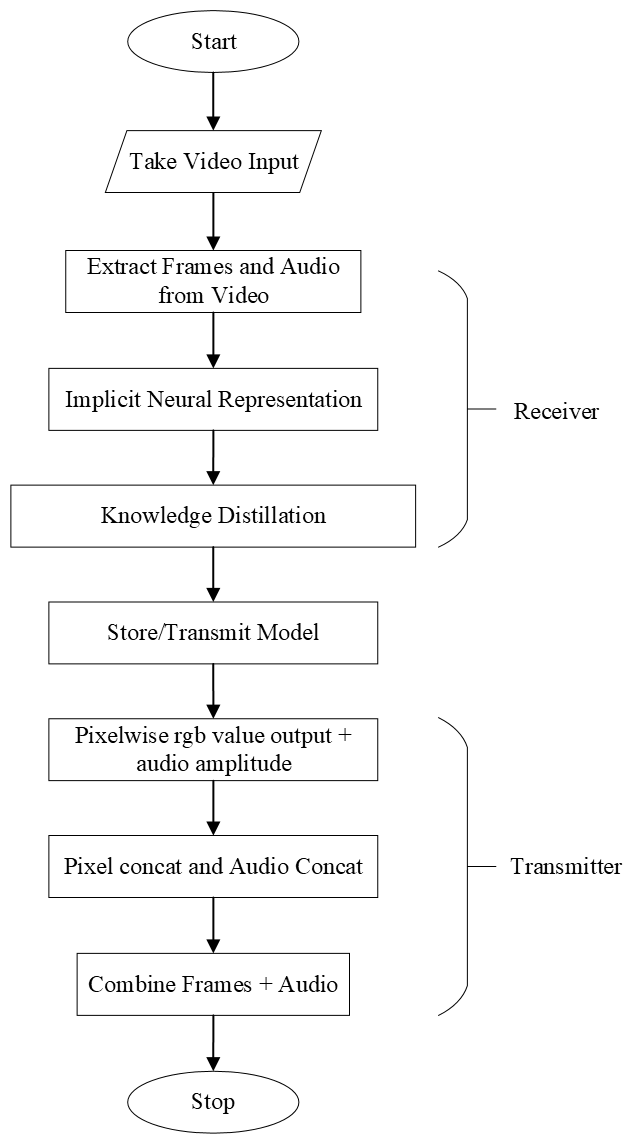
\includegraphics[height=0.7\textheight]{assets/Major Compression Decompression Flowchart.png}
        \caption{Compression Decompression Flowchart}
        \label{fig:comp-decomp-flowchart}
    \end{figure}
    \autoref{fig:comp-decomp-flowchart} describes the overall project flow starting with video input, from which individual frames and audio are extracted. A neural network is trained to model the video, known as implicit neural representation, where a space-time coordinate is mapped to an \gls{rgb} value and an audio amplitude. This trained model undergoes compression using knowledge distillation. The compressed model can then be used for storage or transmission.

    In the Receiver side, the process begins by sampling the model using space-time coordinatres from which \gls{rgb} and amplitude values can be retrieved. The model is sampled multiple times until all frames and audio are fully generated through pixel concatenation and audio concatenation. Finally, the frames and audio are combined to reconstruct the original input video.

    \subsection{Quantization Aware Pruning}
    \textit{Quantization} in machine learning is the process of reducing the number of bits that represent the model's weights and activations. It typically involves converting 32-bit floating-point numbers to lower precision formats like 16-bit, 8-bit, or even binary (1-bit) representations. This reduces the model size and accelerates inference on hardware with limited computational resources.

    \textit{Pruning} is the technique of removing less important weights or neurons from a neural network to make it smaller and faster without significantly affecting performance. This can be achieved by setting the weights that contribute the least to the output to zero, effectively removing connections or neurons.

    \textit{Quantization Aware Pruning} combines both quantization and pruning to further optimize neural networks. This approach considers the effects of quantization during the pruning process, allowing the model to retain accuracy even after both compression techniques are applied. By integrating quantization awareness, the pruning algorithm can make more informed decisions about which weights to prune, considering the eventual lower precision representation of the weights.

    Quantization Aware Pruning typically involves:
    \begin{enumerate}[label=\textbf{\roman*.}]
        \item Training a model with quantization in mind.
        \item Pruning the model while simulating the effects of quantization.
        \item Fine-tuning the pruned and quantized model to recover any lost accuracy.
    \end{enumerate}


    \autoref{fig:quantization-aware-pruning} depicts a comprehensive workflow for Quantization Aware Pruning (QAP) of a neural network. Here's a step-by-step explanation of the process as illustrated:    
    \begin{enumerate}[label=\textbf{\roman*.}]
        \item \textbf{Pre-Trained Model}: The process starts with a pre-trained model that serves as the baseline for further optimization.
        
        \item \textbf{Define Quantization and Pruning Parameters}: Parameters for quantization (e.g., bit-width) and pruning (e.g., threshold for pruning) are defined. These parameters guide the subsequent steps.
        
    \begin{figure}[H]
        \centering
        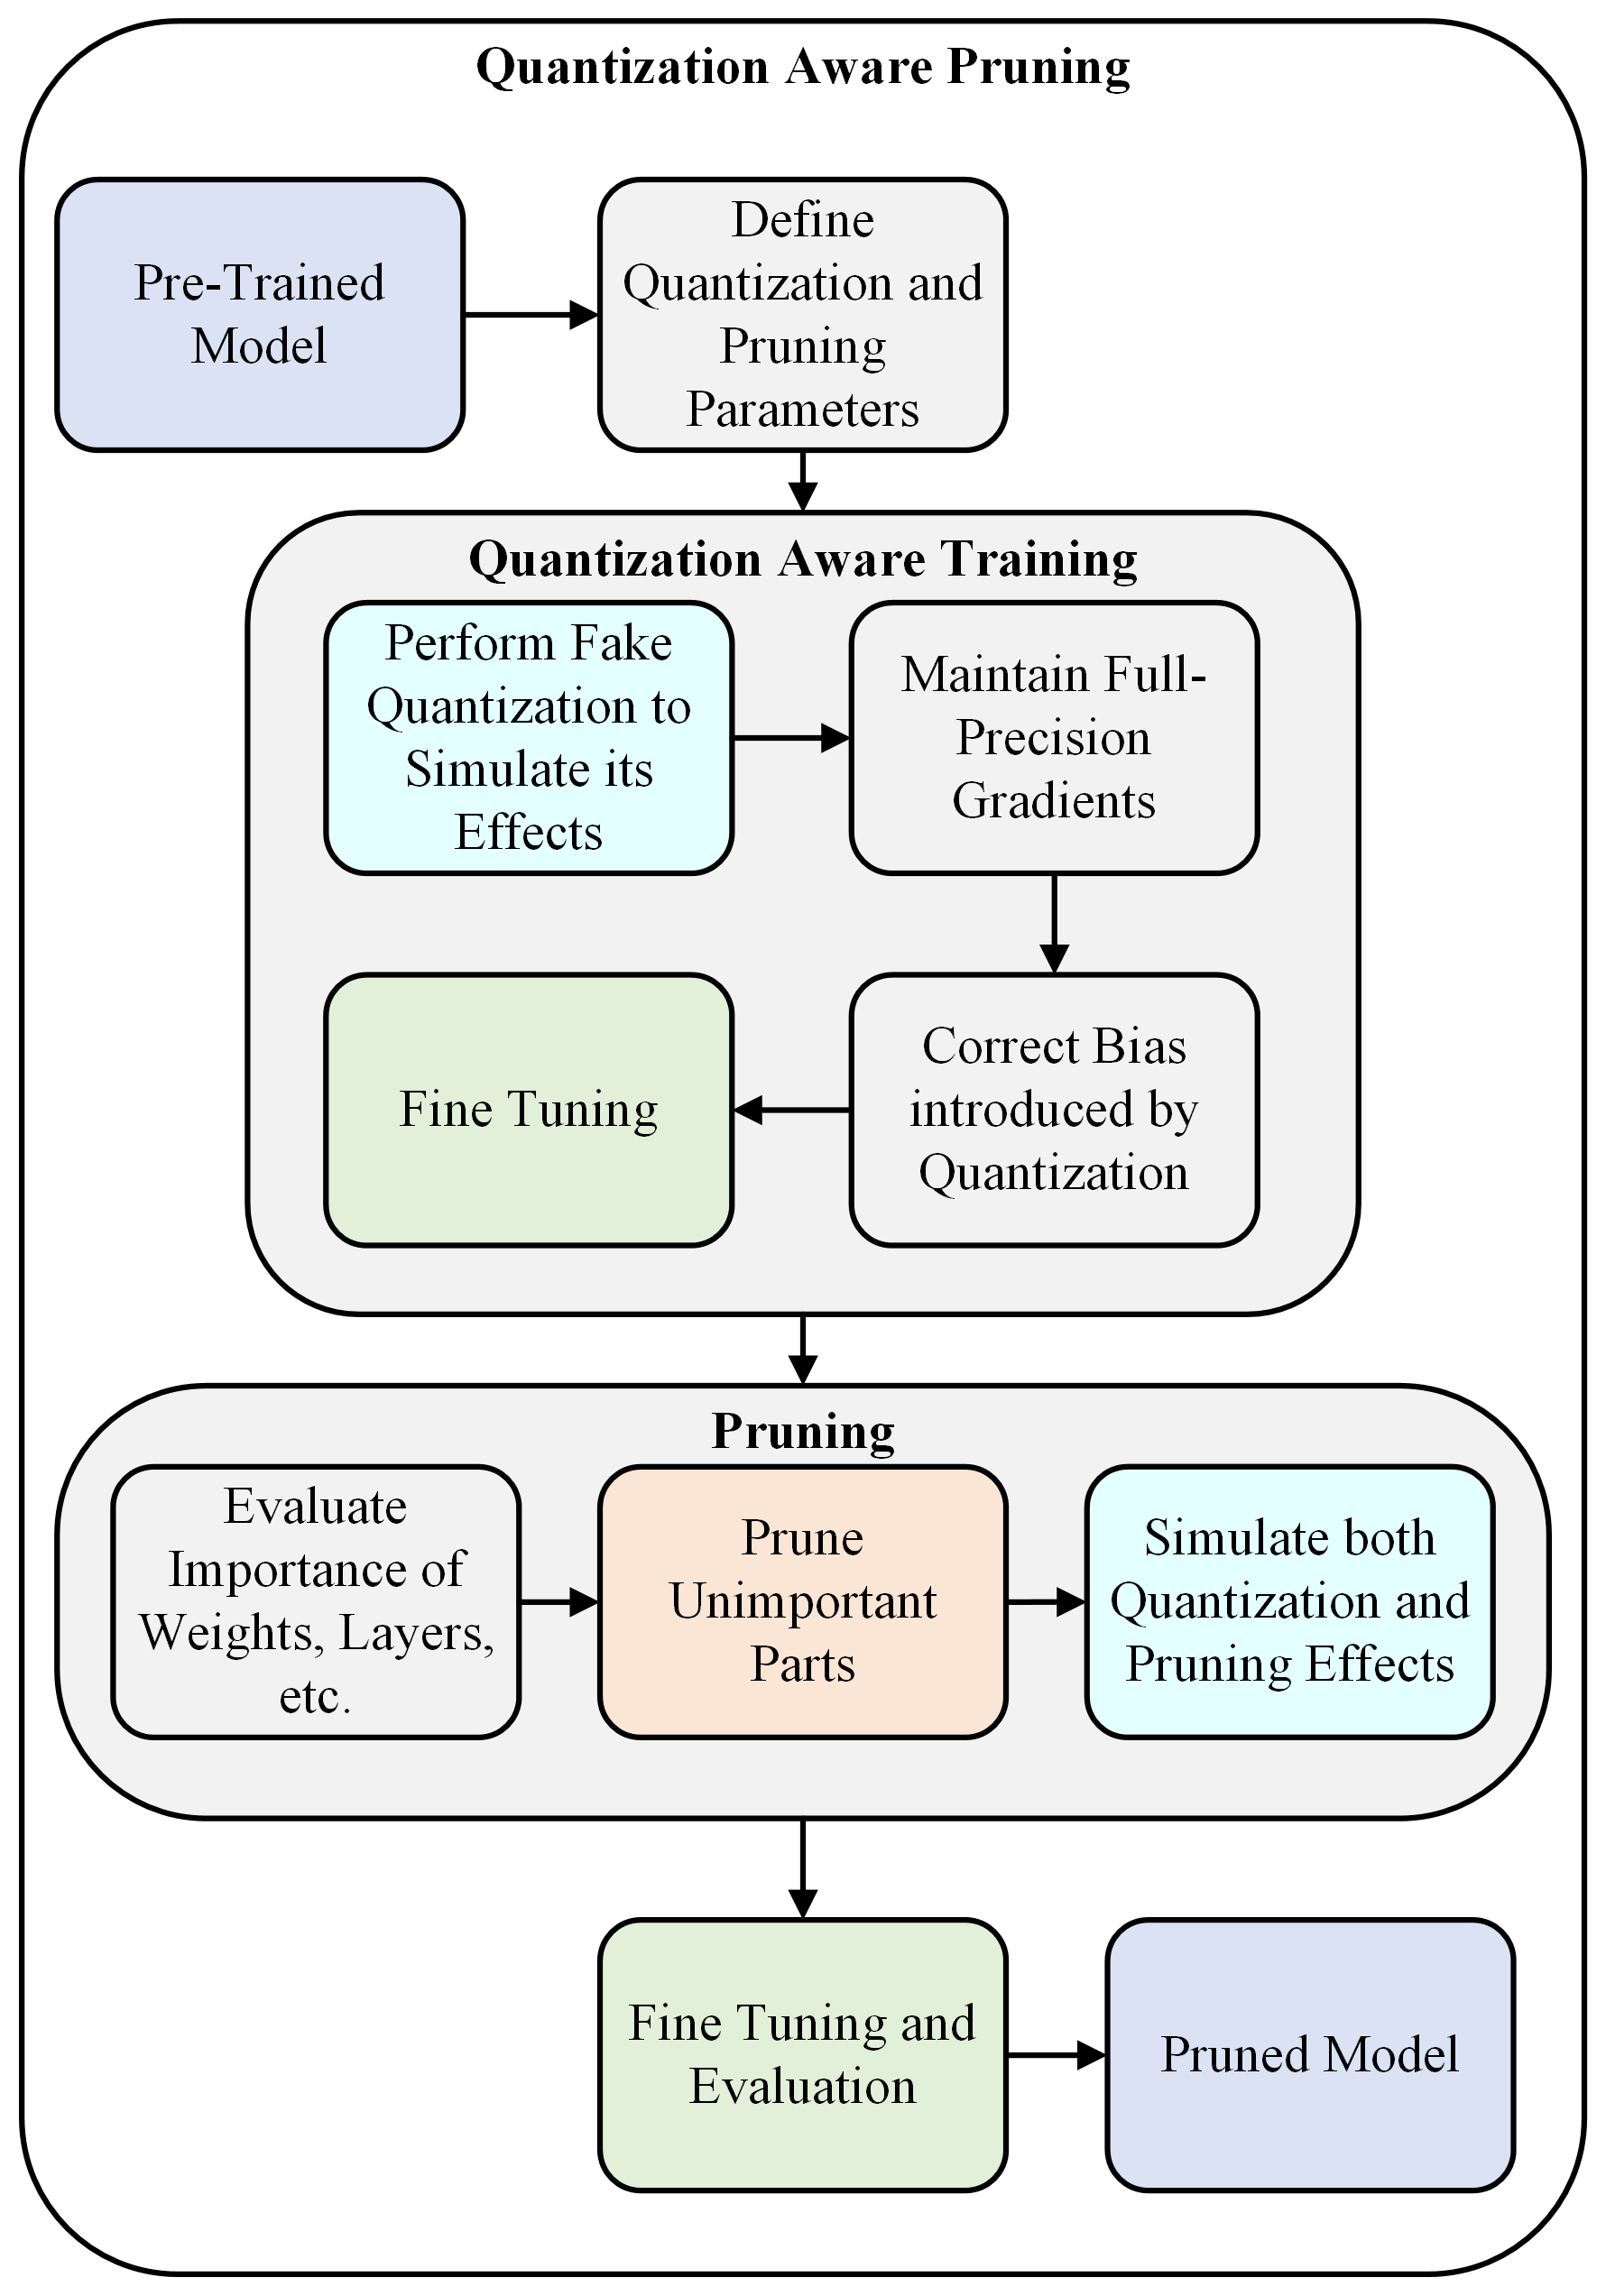
\includegraphics[width=0.9\linewidth]{assets/Quantization Aware Pruning.png}
        \caption{Quantization Aware Pruning}
        \label{fig:quantization-aware-pruning}
    \end{figure}

        \item \textbf{Perform Fake Quantization to Simulate its Effects}: During training, fake quantization is performed to simulate the effects of quantization without actually converting weights to lower precision. This helps the model learn to cope with the reduced precision.
        
        \item \textbf{Maintain Full-Precision Gradients}: While performing fake quantization, gradients are maintained in full precision to ensure stable training.
        
        \item \textbf{Correct Bias introduced by Quantization}: Biases introduced by the fake quantization process are corrected to minimize performance degradation.
        
        \item \textbf{Fine Tuning}: The model undergoes fine-tuning to adapt to the effects of quantization, ensuring that the performance remains optimal.

        \item \textbf{Evaluate Importance of Weights, Layers, etc.}: The importance of different weights and layers is evaluated to identify which parts of the model can be pruned.
        
        \item \textbf{Prune Unimportant Parts}: The identified unimportant parts (e.g., weights, neurons) are pruned to reduce the model size.
        
        \item \textbf{Simulate both Quantization and Pruning Effects}: The combined effects of both quantization and pruning are simulated to assess their impact on the model.
        
        \item \textbf{Fine Tuning and Evaluation}: The pruned model is fine-tuned and evaluated to ensure it performs well despite the reductions in precision and structure.

        \item \textbf{Pruned Model}: The final outcome is a pruned and quantized model that is smaller, faster, and more efficient for deployment on resource-constrained devices.
    \end{enumerate}

    
    \autoref{alg:model-quantization} outline the process of model quantization, which aims to reduce the precision of neural network weights to improve efficiency. The process begins with a trained neural network model. The first step is to choose a quantization scheme, which can be either uniform quantization, where weights are mapped to fixed, uniformly distributed levels, or non-uniform quantization, where techniques like k-means clustering are used to determine the mapping. Following this, the number of quantization levels $Q$ is determined (e.g., 8-bit, 16-bit). Each weight $W_{ij}$ in the model is then mapped to the nearest quantization level within $Q$. The original weights $W$ are replaced with these quantized weights, resulting in a quantized model. Optionally, the quantized model can be fine-tuned on the training dataset to recover any lost accuracy. The final step is to return the quantized model $Q(W)$. This approach effectively reduces the model's memory footprint and potentially improves its computational efficiency while maintaining its performance.
    
    \begin{algorithm}[H]
        \caption{Model Quantization}
        \label{alg:model-quantization}
        \begin{algorithmic}[1]
            \Procedure{Quantize\_Model}{}
            \State Define the neural network model with weights $W$
            \State Train the model on the training dataset
            \State Choose a quantization scheme:
            \State \hspace{\algorithmicindent} a. Uniform quantization: Map weights to fixed levels uniformly distributed.
            \State \hspace{\algorithmicindent} b. Non-uniform quantization: Use techniques like k-means clustering.
            \State Determine the number of quantization levels $Q$ (e.g., 8-bit, 16-bit)
            \For{each weight $W_{ij}$ in $W$}
                \State Map $W_{ij}$ to the nearest quantization level in $Q$
            \EndFor
            \State Replace original weights $W$ with quantized weights $Q(W)$
            \State Optionally, fine-tune the quantized model on the training dataset
            \State \textbf{return} $Q(W)$
            \EndProcedure
        \end{algorithmic}
    \end{algorithm}

    The process as shown in \autoref{alg:model-pruning} begins with a neural network whose weights are denoted by \( W \). The algorithm executes in a loop where several key steps are performed. Firstly, the importance of each weight \( W_{ij} \) is calculated using methods like magnitude, sensitivity analysis, or gradient-based techniques. These methods assess the significance of each weight in terms of its impact on the network’s performance. Subsequently, a pruning threshold \( T \) is established, typically set at a percentile of the importance values, which determines the weights considered less significant and therefore set to zero. After pruning, the network is fine-tuned by retraining on the training dataset to recover any accuracy loss due to the removal of weights, helping the network adjust to its new reduced structure. Optionally, if further complexity reduction is desired without significantly compromising performance, the pruning and fine-tuning steps are repeated iteratively. Each iteration may adjust the pruning threshold or the criteria for weight importance based on performance metrics from the previous iteration. Ultimately, the algorithm returns the pruned network, which is simpler and potentially faster at inference while maintaining adequate performance. The iterative aspect allows for gradual refinement, balancing complexity reduction and performance retention.

    \begin{algorithm}[H]
        \caption{Model Pruning}
        \label{alg:model-pruning}
        \begin{algorithmic}[1]
            \Procedure{Prune\_Model}{}
            \State Let $W$ be the network weights
            \State Train the model on the training dataset
            \Loop
                \State Compute importance of each weight $W_{ij}$
                \State Set a pruning threshold $T$ (e.g., a percentile of weight importance)
                \For{each weight $W_{ij}$ in $W$}
                    \If{importance($W_{ij}$) $<$ $T$}
                        \State Set $W_{ij}$ to 0
                    \EndIf
                \EndFor
                \State Fine-tune the pruned model on the training dataset
                \State If desired, repeat steps 5-10 for iterative pruning
            \EndLoop
            \State \textbf{return} $W$
            \EndProcedure
        \end{algorithmic}
    \end{algorithm}

    
    \subsection{Architecture of Neural Network}
    \begin{figure}[H]
        \centering
        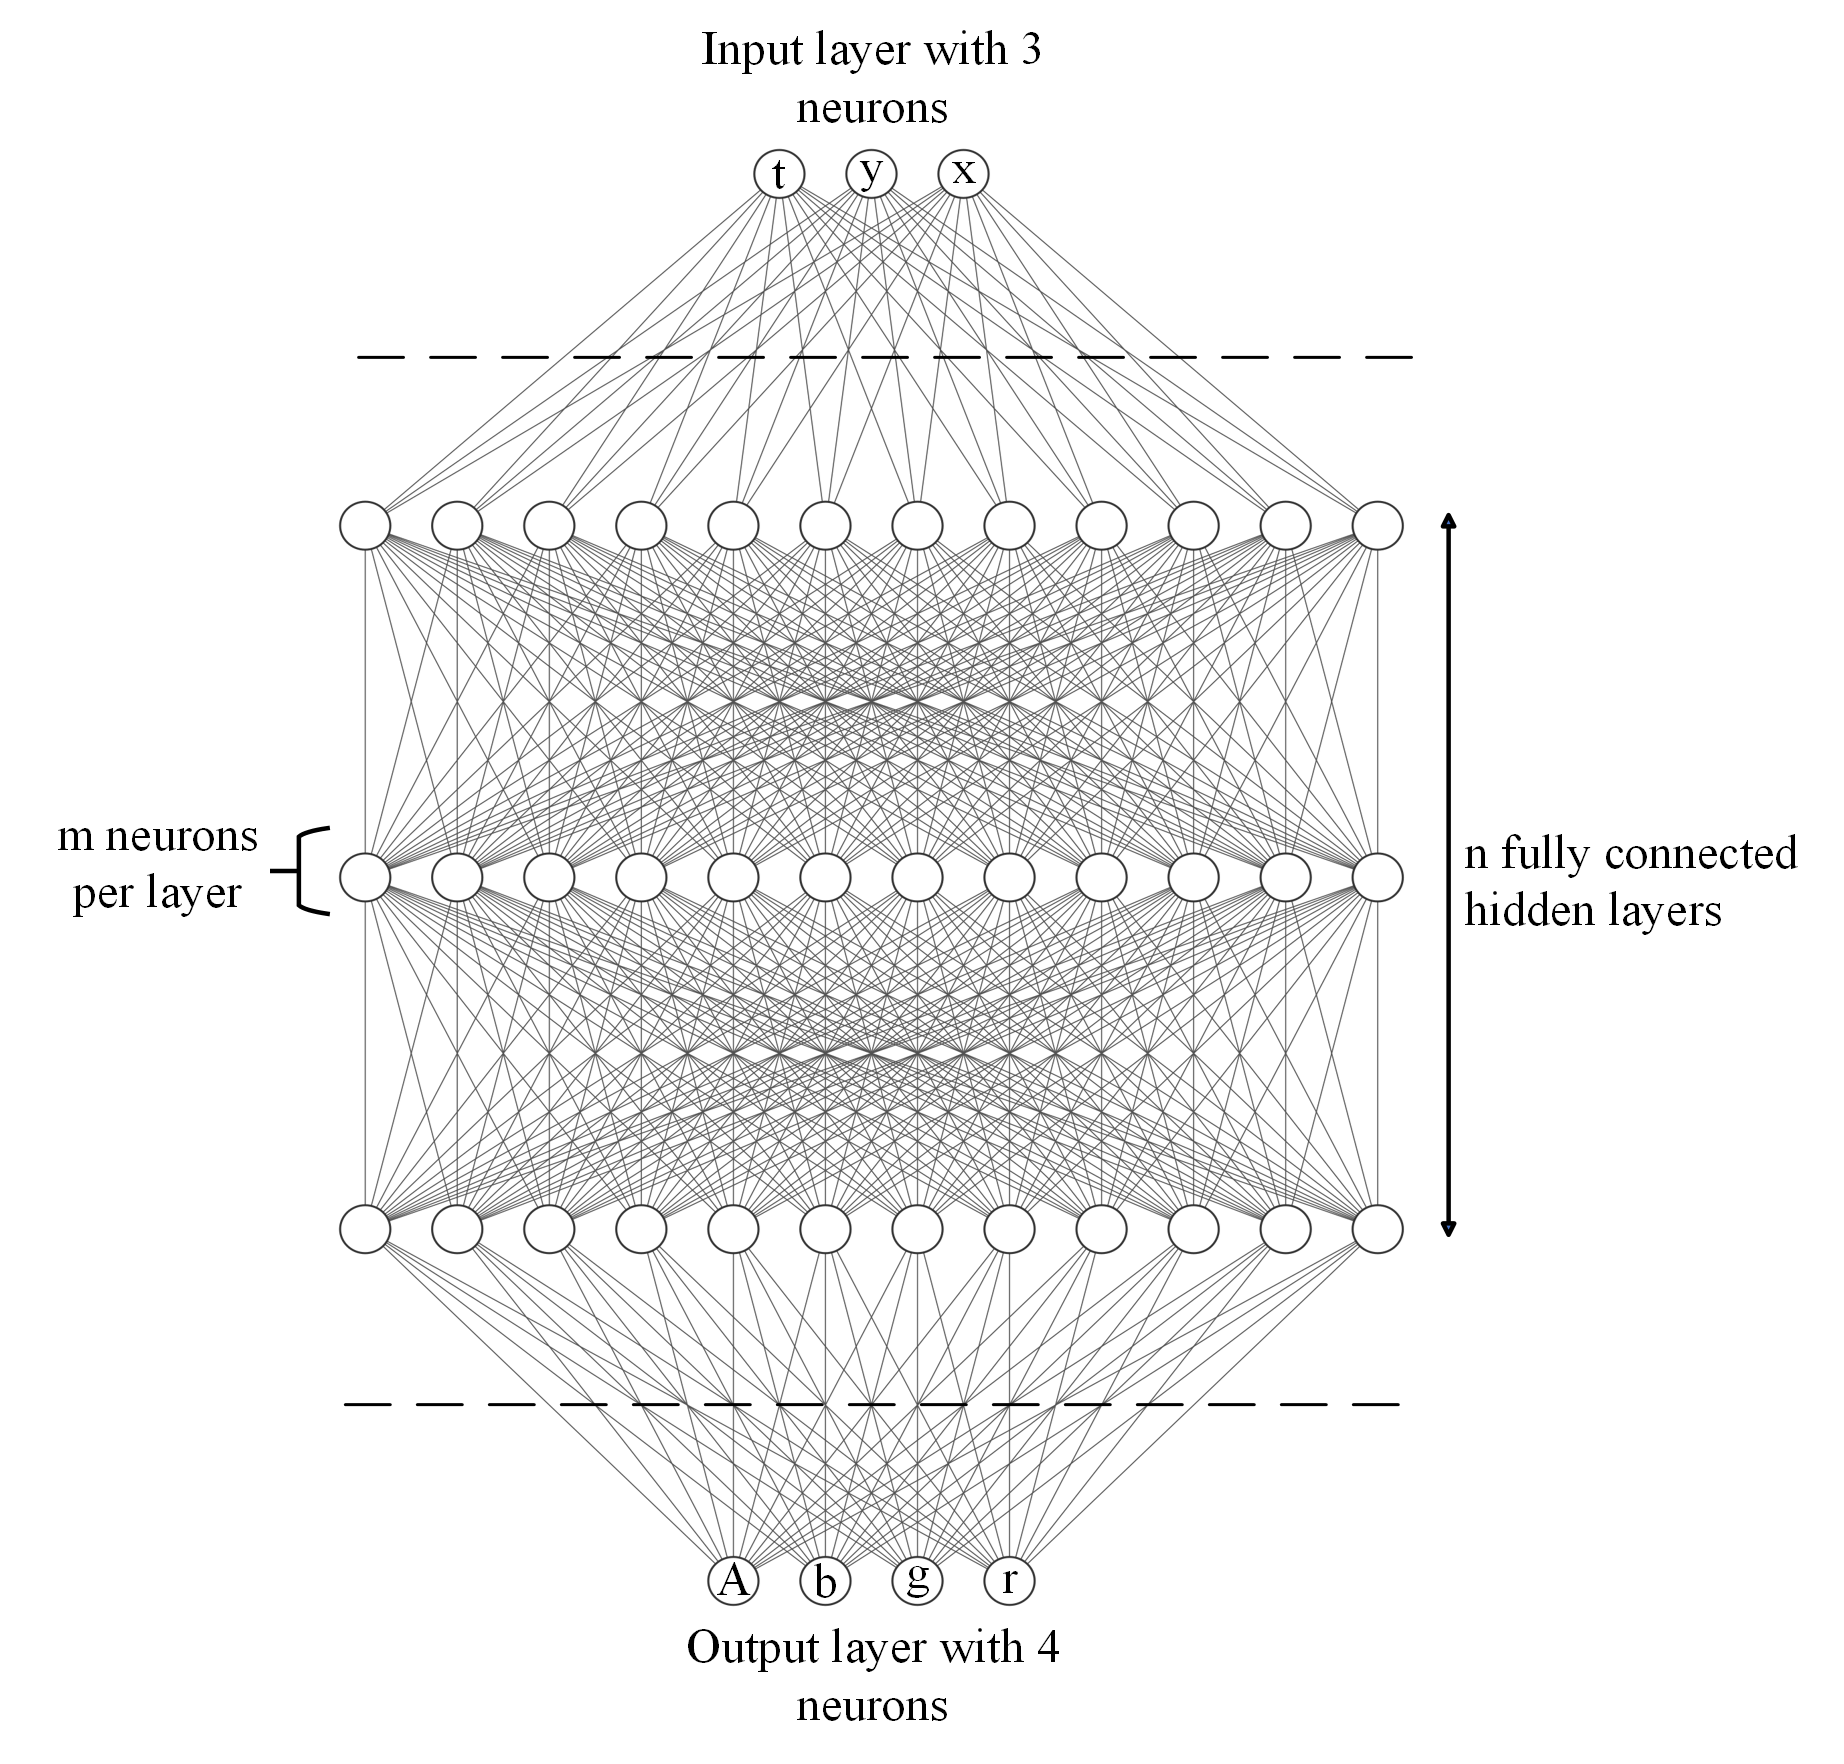
\includegraphics[height=0.6\textheight]{assets/Neural Network Architecture Vertical.png}
        \caption{Architecture of Neural Network}
        \label{fig:architecture-neural-network}
    \end{figure}
    The neural network model is designed to process spatio-temporal coordinates and generate corresponding \gls{rgb} pixel values and audio amplitude. The network features an input layer with 3 neurons, which takes in the space-time coordinates $(x, y, t)$ where $x$ and $y$ are spatial coordinates and $t$ is the temporal coordinate. The output layer consists of 4 neurons that produce the RGB values of a pixel and the amplitude value of audio, specifically the Red ($r$), Green ($g$), and Blue ($b$) color values, along with the audio amplitude ($A$). Between the input and output layers, the model includes $n$ fully connected hidden layers, each containing $m$ neurons. Each of these layers employs the \gls{siren} activation function, which uses the sine function to effectively model periodic signals and fine-grained details, making it particularly suitable for handling the intricate relationships inherent in audio and visual data. This architecture uses the SIREN activation function to enable high-quality signal representation, capturing both spatial and temporal dynamics to generate detailed multimedia outputs.
    
    \subsection{Loss Function}
    To effectively generate \gls{inr} for audio-video data, it is essential to define appropriate loss functions that guide the learning process. Below, the specific loss functions for audio and video are introduced, followed by the formulation of a combined loss function that integrates both modalities.

        \subsubsection{Audio Loss Function}
        The loss function for audio data is defined as:
        \begin{equation}
            \mathcal{L}_{\text{audio}} = \int_{\Omega_{\text{audio}}} \| \Phi_{\text{audio}}(t) - f_{\text{audio}}(t) \| \, dt
        \end{equation}
        where:
        \begin{itemize}
            \item \( t \in \mathbb{R} \) is the time point,
            \item  \( \Phi_{\text{audio}}(t) \) is the model's output for the audio at time \( t \),
            \item \( f_{\text{audio}}(t) \) is the ground truth audio amplitude at time \( t \),
            \item \( \Omega_{\text{audio}} \) is the time interval over which the audio is defined.
        \end{itemize}
    
        \subsubsection{Video Loss Function}
            The loss function for video data is defined as:
        \begin{equation}
            \mathcal{L}_{\text{video}} = \int_{\Omega_{\text{video}}} \| \Phi_{\text{video}}(x, t) - f_{\text{video}}(x, t) \| \, dx \, dt
        \end{equation}
        where:
        \begin{itemize}
        \item \( (x, t) \in \mathbb{R}^3 \) represents the space-time coordinates,
        \item \( \Phi_{\text{video}}(x, t) \) is the model's output for the video at space-time coordinate \( (x, t) \),
        \item \( f_{\text{video}}(x, t) \) is the ground truth RGB value at space-time coordinate \( (x, t) \),
        \item \( \Omega_{\text{video}} \) is the space-time region over which the video is defined.
        \end{itemize}
    
        \subsubsection{Combined Loss Function}
        The combined loss function for both audio and video data is formulated as:
        \begin{equation}
            \mathcal{L}_{\text{combined}} = \lambda_{\text{audio}} \mathcal{L}_{\text{audio}} + \lambda_{\text{video}} \mathcal{L}_{\text{video}}
            \end{equation}
            where:
            \begin{itemize}
                \item \( \lambda_{\text{audio}} \) is the weight that balances the contribution of the audio loss,
                \item \( \lambda_{\text{video}} \) is the weight that balances the contribution of video loss.
            \end{itemize}
    This combined loss function ensures that both the audio and video outputs are supervised and optimized simultaneously.
    
    \subsection{Evaluation Metrics for Video}
        To rigorously evaluate the effectiveness of our proposed INR based video compression technique, we will utilize a suite of metrics that assess various dimensions of video quality, including visual fidelity, perceptual quality, and predictive accuracy. Here's an overview of each metric, their numerical value ranges, and whether it's preferable for their values to increase or decrease:
        \subsubsection{Peak Signal-to-Noise Ratio}
            \begin{itemize}
                \item \textbf{Overview}: \gls{psnr} is commonly employed to measure the quality of reconstruction in lossy compression \gls{codec}s. It compares the similarity between the original and compressed video by measuring the ratio between the maximum possible power of a signal and the power of distorting noise.
                \item \textbf{Value Range}: Typically expressed in \gls{db}, the higher the \gls{psnr}, the better the quality of the compressed video. A higher \gls{psnr} value indicates that the reconstruction is of higher quality.
                \item \textbf{Preference} $\uparrow$: Values typically range from 20 to 50 \gls{db}, where higher values (around 40 \gls{db} or more) represent excellent quality.
                \item \textbf{Formula} \\ 
                \begin{equation}\label{eqn:PSNR}
                    \text{PSNR} = 20 \cdot \log_{10}\left(\frac{{\text{MAX}_I}}{\sqrt{\text{MSE}}}\right)
                \end{equation}
                where $\text{MAX}_I$ is the maximum possible pixel value of the image (e.g., 255 for 8-bit images), and $\text{MSE}$ is the mean squared error between the original and compressed image.
               \end{itemize} 
           
        \subsubsection{Learned Perceptual Image Patch Similarity}
            \begin{itemize}
                \item \textbf{Overview}: \gls{lpips} metric evaluates the perceptual difference between two images or videos. Unlike traditional metrics that focus on pixel-level accuracy, \gls{lpips} uses deep learning to assess how perceptually similar two images are to the human eye.
                \item \textbf{Value Range}: This metric produces a similarity score that ranges from 0 to 1, where lower scores indicate greater perceptual similarity.
                \item \textbf{Preference} $\downarrow$: A lower \gls{lpips} score means that the compressed video is perceptually closer to the original, indicating better compression performance.
            \end{itemize}

        \subsubsection{Structural Similarity Index Measure}
            \begin{itemize}
                \item \textbf{Overview}: \gls{ssim} is used to measure the similarity between two images or videos. It considers attributes that are important to the human visual system such as luminance, contrast, and structure.
                \item \textbf{Value Range}: \gls{ssim} values range from -1 to 1. A score of 1 indicates perfect similarity, meaning there is no loss of structural information.
                \item \textbf{Preference} $\uparrow$: Higher \gls{ssim} values signify less visual distortion and better compression quality.
                \item \textbf{Formula}\\ 
                \begin{equation}\label{eqn:SSIM}
                    \text{SSIM}(x, y) = \frac{(2 \mu_x \mu_y + c_1)(2 \sigma_{xy} + c_2)}{(\mu_x^2 + \mu_y^2 + c_1)(\sigma_x^2 + \sigma_y^2 + c_2)}
                \end{equation}
                where $\mu_x$ and $\mu_y$ are the average intensities of images $x$ and $y$, $\sigma_{x}$ and $\sigma_y$ are the variance, $\sigma_{xy}$ is the covariance between $x$ and $y$, and $c_1$ and $c_2$ are variables to stabilize division.
            \end{itemize}

        
        \subsubsection{L1 Loss / Mean Absolute Error}
            \begin{itemize}
                \item \textbf{Overview}: L1 loss measures the average magnitude of errors between corresponding pixels in the original and compressed images or frames, without considering the direction of the errors.
                \item \textbf{Value Range}: The value can range from 0 to $\infty$,  0 indicating no error (perfect compression).
                \item \textbf{Preference} $\downarrow$: Lower L1 loss values indicate that the compressed video is more accurate in terms of raw pixel values.
                \item \textbf{Formula}\\
                \begin{equation}
                    \text{MAE} = \frac{1}{N} \sum_{i=1}^{N} |x_i - y_i|
                \end{equation}
                where $x_i$ and $y_i$ are pixel values of original and compressed images respectively, and $N$ is the total number of pixels.
            \end{itemize}


        \subsubsection{File Size}
            \begin{itemize}
                \item \textbf{Overview}: File size measures the total amount of storage space required by a compressed video file. It is a direct indicator of the efficiency of a compression technique.
                \item \textbf{Value Range}: File size is typically measured in bytes, \gls{kb}, \gls{mb}, or \gls{gb}. The value range can vary widely depending on the length and resolution of the video.
                \item \textbf{Preference} $\downarrow$: Lower file sizes are preferable as they indicate more efficient compression.
            \end{itemize}

        \subsubsection{Bandwidth Usage}
            \begin{itemize}
                \item \textbf{Overview}: Bandwidth usage measures the amount of data transmitted over a network to stream or download a video. It evaluates the feasibility of video transmission in various network conditions.
                \item \textbf{Value Range}:  Bandwidth usage is typically measured in \gls{bps},\gls{kbps}, or \gls{mbps}. The value range can vary depending on the video quality and compression efficiency.
                \item \textbf{Preference} $\downarrow$: Lower bandwidth usage is preferable as it indicates more efficient data transmission.
            \end{itemize}

        \subsubsection{Encoding/Decoding Time}
        \begin{itemize}
            \item \textbf{Overview}: Encoding/decoding time measures the time required to compress (encode) or decompress (decode) a video file. It is a critical factor in real-time applications and systems with limited processing capabilities.
            \item \textbf{Value Range}: Encoding/decoding time is typically measured in seconds or milliseconds. The exact value can vary widely depending on the complexity of the video content.
            \item \textbf{Preference} $\downarrow$: Lower encoding/decoding times are preferred, as they indicate more efficient compression.
        \end{itemize}
\subsection{Evaluation Metrics for Audio}
To thoroughly assess the effectiveness of our proposed audio processing techniques, we will utilize a comprehensive suite of metrics that evaluate various aspects of audio quality, including clarity, fidelity, intelligibility, and perceptual similarity. Here's an overview of each metric, their numerical value ranges, and the preferred direction for their values:

\subsubsection{Log Spectral Distance (LSD)}
\begin{itemize}
    \item \textbf{Overview:} LSD measures the difference between the log magnitude spectra of the reference and processed audio signals, making it sensitive to spectral distortions.
    
    \item \textbf{Value Range:} LSD is typically measured in decibels (dB) and can range from 0 (no spectral distortion) to higher positive values.
    
    \item \textbf{Preference $\downarrow$:} Lower values are preferable, indicating lower spectral distortion.
    
    \item \textbf{Formula:} LSD is computed as:
    \begin{equation}
        \text{LSD} = \frac{1}{N} \sum_{n=1}^{N} \sqrt{\frac{1}{K} \sum_{k=1}^{K} \left[ \log |X(k,n)| - \log |Y(k,n)| \right]^2}
    \end{equation}
    where \( X(k,n) \) and \( Y(k,n) \) are the magnitude spectra of the original and processed signals for the \( n \)-th frame and \( k \)-th frequency bin, respectively, \( N \) is the number of frames, and \( K \) is the number of frequency bins.
\end{itemize}

\subsubsection{Peak Signal-to-Noise Ratio (PSNR)}
\begin{itemize}
    \item \textbf{Overview:} PSNR is a widely used metric to measure the quality of reconstruction of lossy compression codecs. It represents the ratio between the maximum possible power of a signal and the power of corrupting noise.
    
    \item \textbf{Value Range:} PSNR is expressed in decibels (dB) and typically ranges from 20 to 50 dB, with higher values indicating better quality.
    
    \item \textbf{Preference $\uparrow$:} Higher values are preferable, indicating less noise and better signal reconstruction quality.
    
    \item \textbf{Formula:} PSNR is calculated as:
    \begin{equation}
        \text{PSNR} = 20 \cdot \log_{10}\left(\frac{{\text{MAX}_I}}{\sqrt{\text{MSE}}}\right)
    \end{equation}
    where \( MAX \) is the maximum possible pixel value (in audio, the signal's peak value), and MSE is the mean squared error between the original and processed audio signals.
\end{itemize}

\subsubsection{File Size}
            \begin{itemize}
                \item \textbf{Overview}: File size measures the total amount of storage space required by a compressed video file. It is a direct indicator of the efficiency of a compression technique.
                \item \textbf{Value Range}: File size is typically measured in bytes, \gls{kb}, \gls{mb}, or \gls{gb}. The value range can vary widely depending on the length and resolution of the video.
                \item \textbf{Preference} $\downarrow$: Lower file sizes are preferable as they indicate more efficient compression.
            \end{itemize}


    \pagebreak

    \subsection*{KL Divergence and Earth Mover's Distance}

    \subsubsection*{KL Divergence}
    KL Divergence (Kullback-Leibler Divergence) is a measure of how one probability distribution diverges from a second, expected probability distribution. It quantifies the difference between two distributions \( P \) and \( Q \).
    
    \begin{equation}
        D_{KL}(P \parallel Q) = \sum_{i} P(i) \log \frac{P(i)}{Q(i)}
    \end{equation}
    
    \subsubsection*{Earth Mover's Distance (EMD)}
    Earth Mover's Distance is a measure of the distance between two probability distributions over a region \( D \). It is the minimum cost to transform one distribution into the other, viewed as the "work" needed to move the distribution mass.
    
    \begin{equation}
        \text{EMD}(P, Q) = \inf_{\gamma \in \Gamma(P,Q)} \int_{D \times D} d(x, y) \, d\gamma(x, y)
    \end{equation}
    
    where \( \Gamma(P, Q) \) is the set of all possible joint distributions whose marginals are \( P \) and \( Q \), and \( d(x, y) \) is the ground distance between elements \( x \) and \( y \).
    

\section{\MakeUppercase{Dataset Exploration}}
\autoref{tab:audio_files} provides a summary of various audio files, detailing their serial numbers (SN), file names, sampling rates, file sizes in \gls{kib}, and durations in seconds. A brief description of the audio is mentioned after the table.

\subsection{Audio Dataset}
\begin{table}[H]
\centering
\caption{Audio Files Characteristics}
\label{tab:audio_files}
\begin{tabular}{|c|c|c|c|c|}
    \hline
    \textbf{SN} & \textbf{Audio File} & \textbf{Sampling Rate (Hz)} & \textbf{Size (KiB)} & \textbf{Duration(s)}\\
    \hline
    1 & puretone100hz & 44100 & 516.84 & 6 \\
    \hline
    2 & puretone500hz & 44100 & 516.84 & 6 \\
    \hline
    3 & puretone1000hz & 44100 & 516.84 & 6 \\
    \hline
    4 & puretone5000hz & 44100 & 516.84 & 6 \\
    \hline
    5 & sweeping\_tone200-500hz & 44100 & 516.83 & 6 \\
    \hline
    6 & fluctuating\_tone400 & 44100 & 516.84 & 6 \\
    \hline
    7 & multitoneA4E4 & 44100 & 430.7 & 5\\
    \hline
    8 & multitoneBeats & 44100 & 430.7 & 5\\ 
    \hline
    9 & 06seconds & 44100 & 1203.99 & 6\\
    \hline
    10 & 12seconds & 48000 & 1212.21 & 12\\
    \hline
    11 & 24seconds & 48000 & 4633.97 & 24  \\
    \hline
    12 & music & 44100 & 1033.63 & 6 \\
    \hline
\end{tabular}
\end{table}

    \begin{enumerate}
        \item puretone100hz : Contains a pure tone of frequency 100 hertz.
        \item puretone500hz : Contains a pure tone of frequency 500 hertz.
        \item puretone100hz : Contains a pure tone of frequency 1000 hertz.
        \item puretone5000hz : Contains a pure tone of frequency 5000 hertz. 
        \item sweeping\_tone200-500hz: Contains a sweeping tone starting at 200 hertz and slowly increasing upto 500 hertz.
        \item fluctuating\_tone400 : Contains a repeatedly fluctuating frequency around 400 hertz (\textpm 30 hertz).
        \item multitoneA4E4 : Multitone consisting of frequencies 440 hertz and 660 hertz.
        \item multitoneBeats : Multitone consisting of frequencies 400 and 403 hertz.
        \item 06seconds : A melody played using a violin.
        \item 12seconds : Female commentary with crowd chants in the background for first 4 seconds. For rest of the 7 seconds, a male voice narration with music effects in the background.
        \item 24seconds : Instruments playing a melody for first 19 seconds. For rest of the 5 seconds, a male voice with music effects in the background.
        \item music : A song with male vocalist and multiple instruments.
        
    \end{enumerate}

\subsection{Video Dataset}

\autoref{tab:video_files} provides a summary of various video files, detailing their serial numbers (SN), file names, resolution, frames per second (fps), file size in \gls{mib} and video duration in seconds.

\begin{table}[H]
\centering
\caption{Video Files Characteristics}
\label{tab:video_files}
\begin{tabular}{|c|c|c|c|c|c|}
    \hline
    \textbf{SN} & \textbf{Video File} & \textbf{Resolution} & \textbf{FPS} & \textbf{Size (MiB)} & \textbf{Duration(s)}\\ 
    \hline 
    1 & very\_very\_short\_video & 448 x 256 & 1 & 1.29 & 5\\ 
    \hline 
    2 & very\_short\_video &448 x 256 & 1 & 1.56 & 10\\ 
    \hline 
    3 & short\_video & 448 x 256 & 1 & 4.69 & 30 \\ 
    \hline 
    4 & medium\_video & 448 x 256 & 5.6 & 8.7 & 10\\ 
    \hline 
    5 & long\_video & 448 x 256 & 7 & 10.78 & 10\\ 
    \hline
\end{tabular}
\end{table}

Among the five silent videos, three videos (very\_very\_short\_video, very\_short\_video, and short\_video) have frames without any temporal relationship meaning it is a slideshow video of unrelated images, while the other two videos include some frames that do have a temporal connection.


\subsection{Spatial Frequency and Radial Plots of Frames in Video Dataset}
\begin{figure}[H]
    \centering
    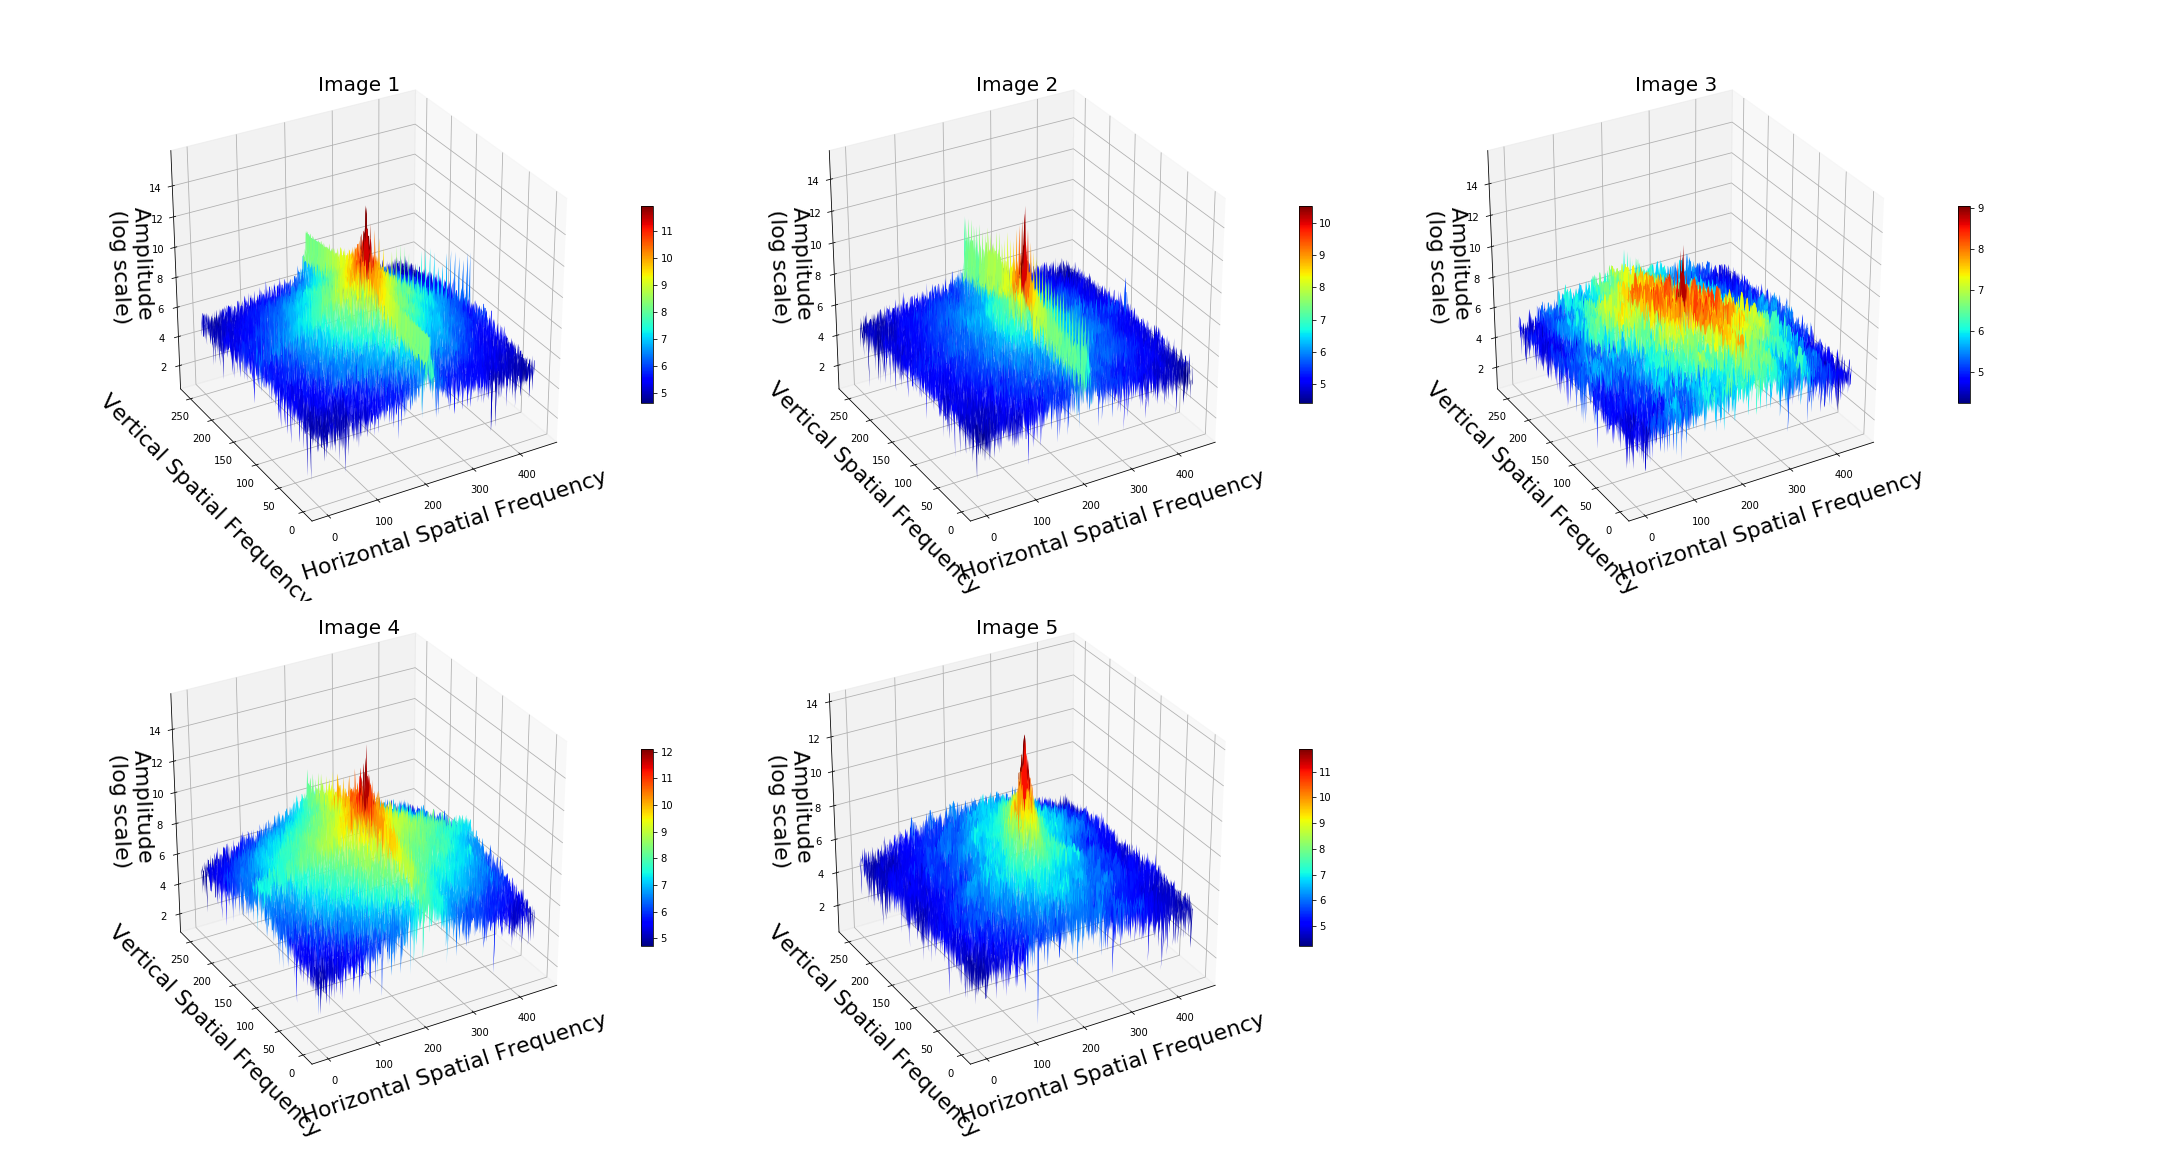
\includegraphics[width=\linewidth]{assets/spatial_frequency/video1spatialfreq.png}
    \caption{Spatial Frequency of all frames of Video 1}
    \label{fig:spatial-frequency-1}
\end{figure}

The above figure contains the spatial frequency graph of all 5 frames of video 1. For the remaining videos in the dataset, we present the spatial frequency graphs for only the frames with the highest and lowest average spatial frequency within each video.

\begin{figure}[H]
    \centering
    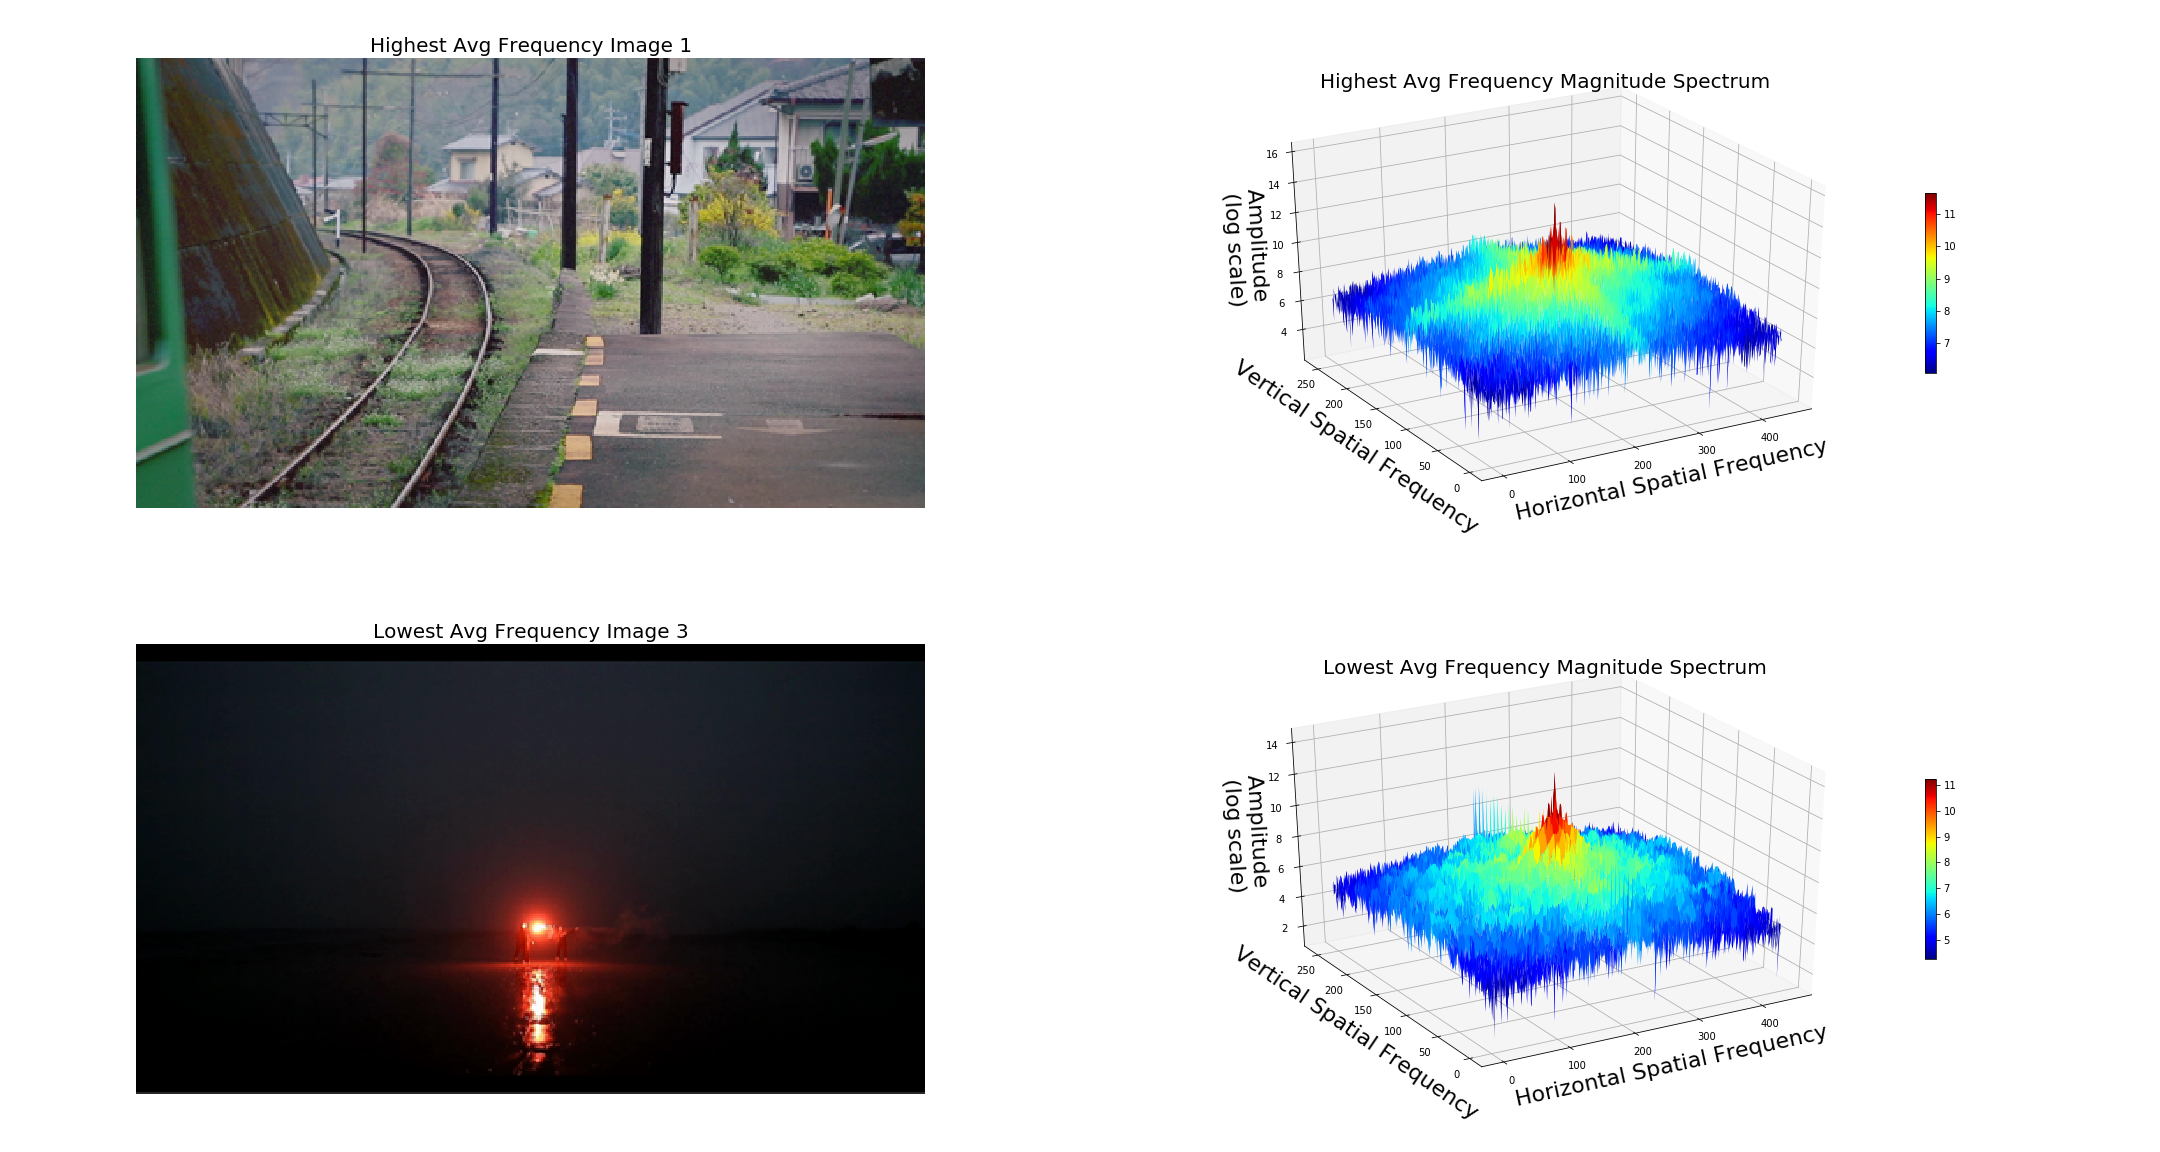
\includegraphics[width=\linewidth]{assets/spatial_frequency/video2spatialfreq.png}
    \caption{Highest and Lowest average Spatial Frequency in Video 2}
    \label{fig:spatial-frequency-2}
\end{figure}

\begin{figure}[H]
    \centering
    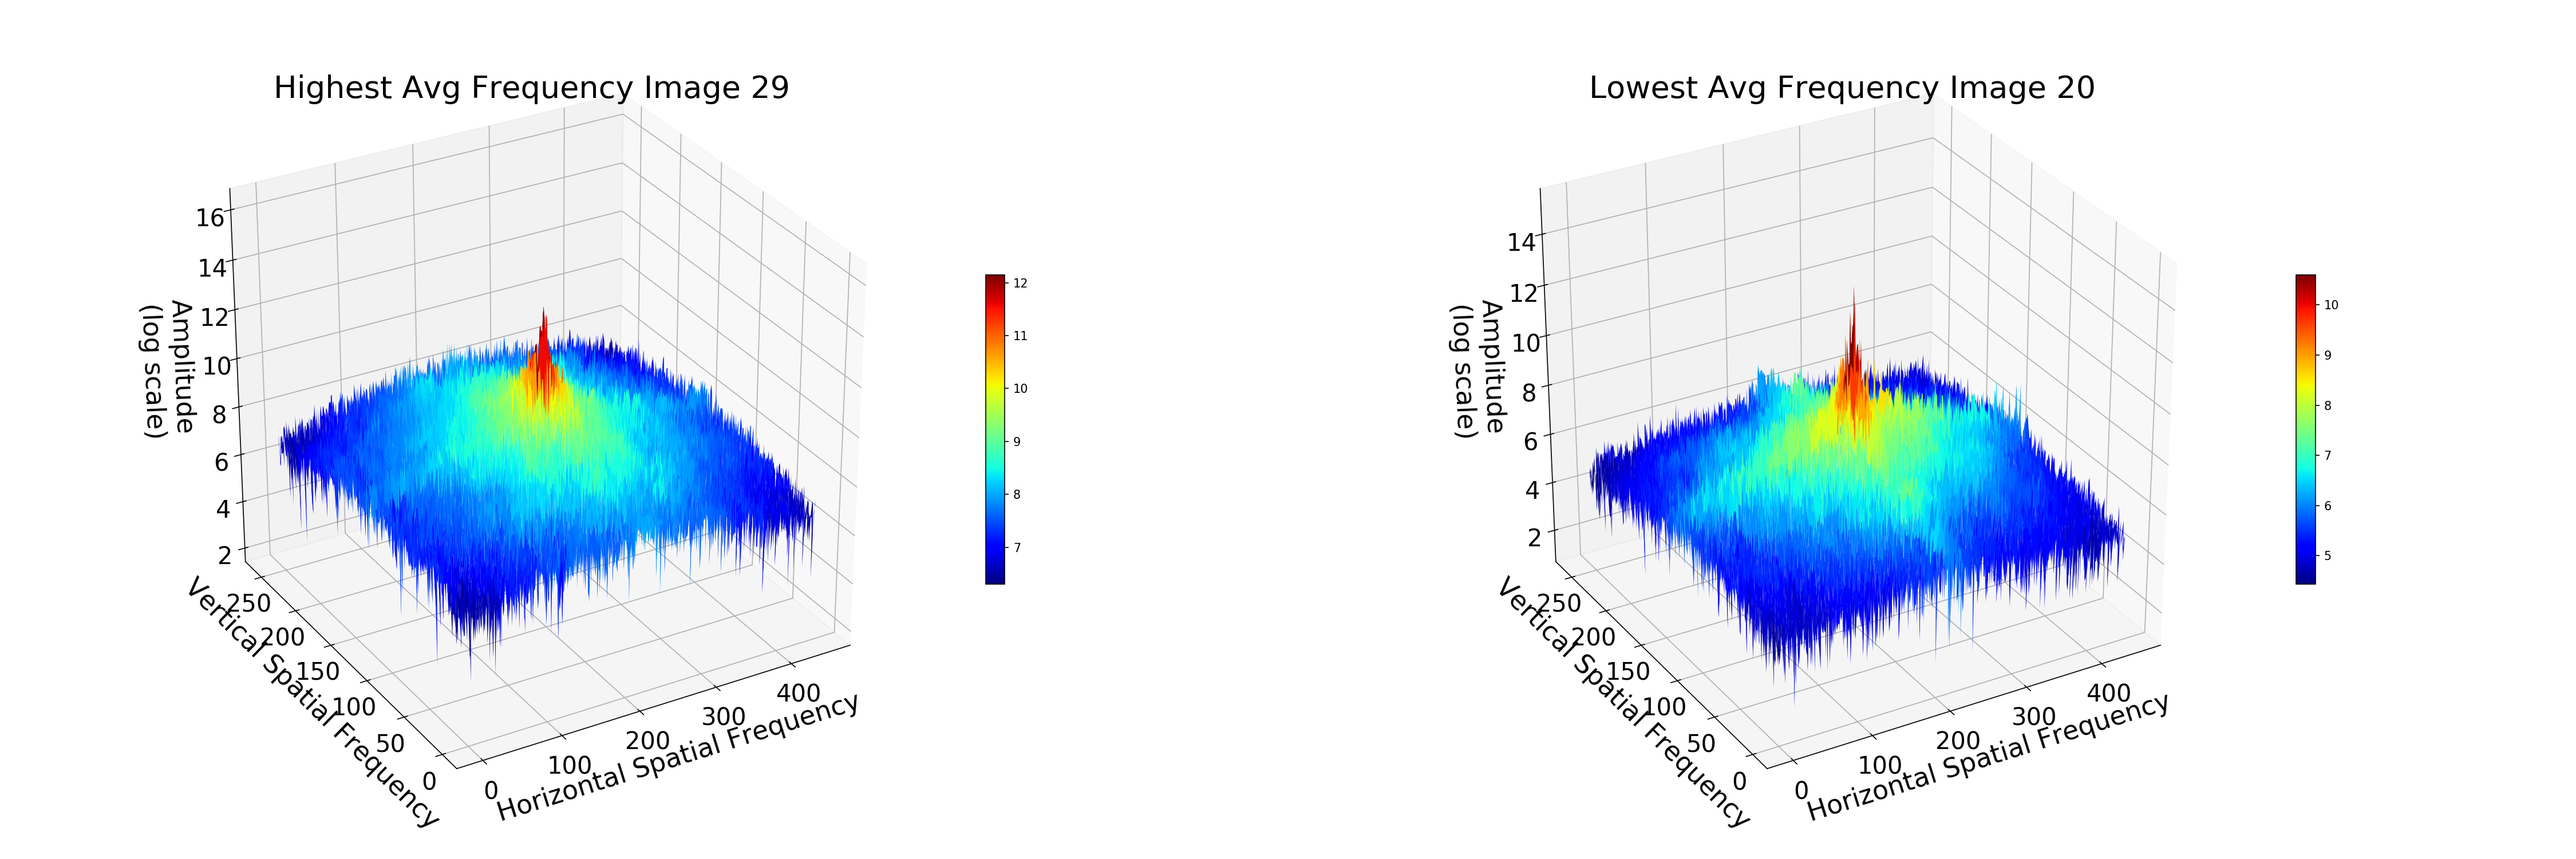
\includegraphics[width=\linewidth]{assets/spatial_frequency/video3spatialfreq.png}
    \caption{Highest and Lowest average Spatial Frequency in Video 3}
    \label{fig:spatial-frequency-3}
\end{figure}

\begin{figure}[H]
    \centering
    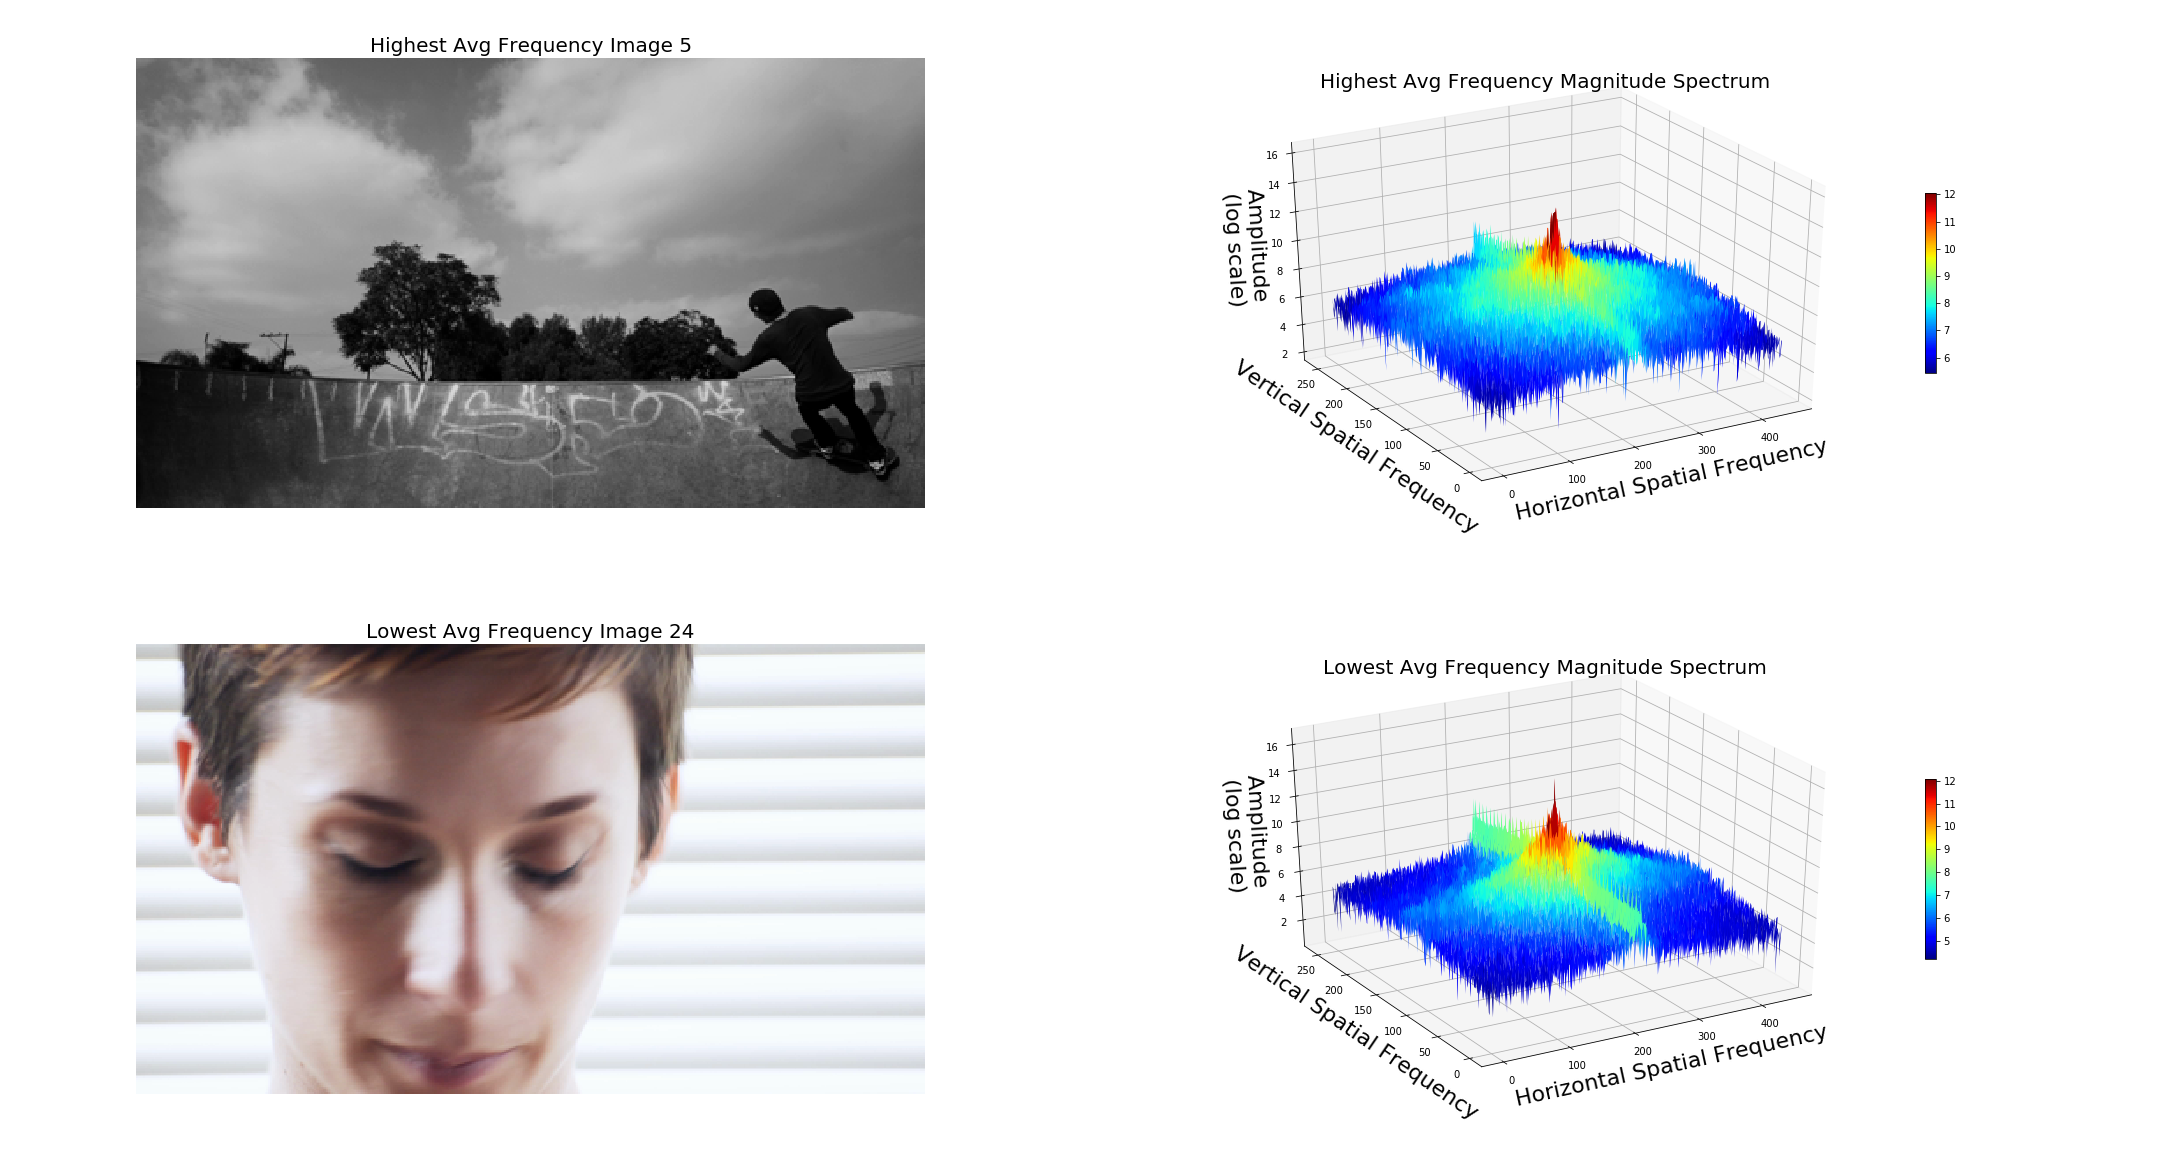
\includegraphics[width=\linewidth]{assets/spatial_frequency/video4spatialfreq.png}
    \caption{Highest and Lowest average Spatial Frequency in Video 4}
    \label{fig:spatial-frequency-4}
\end{figure}

\begin{figure}[H]
    \centering
    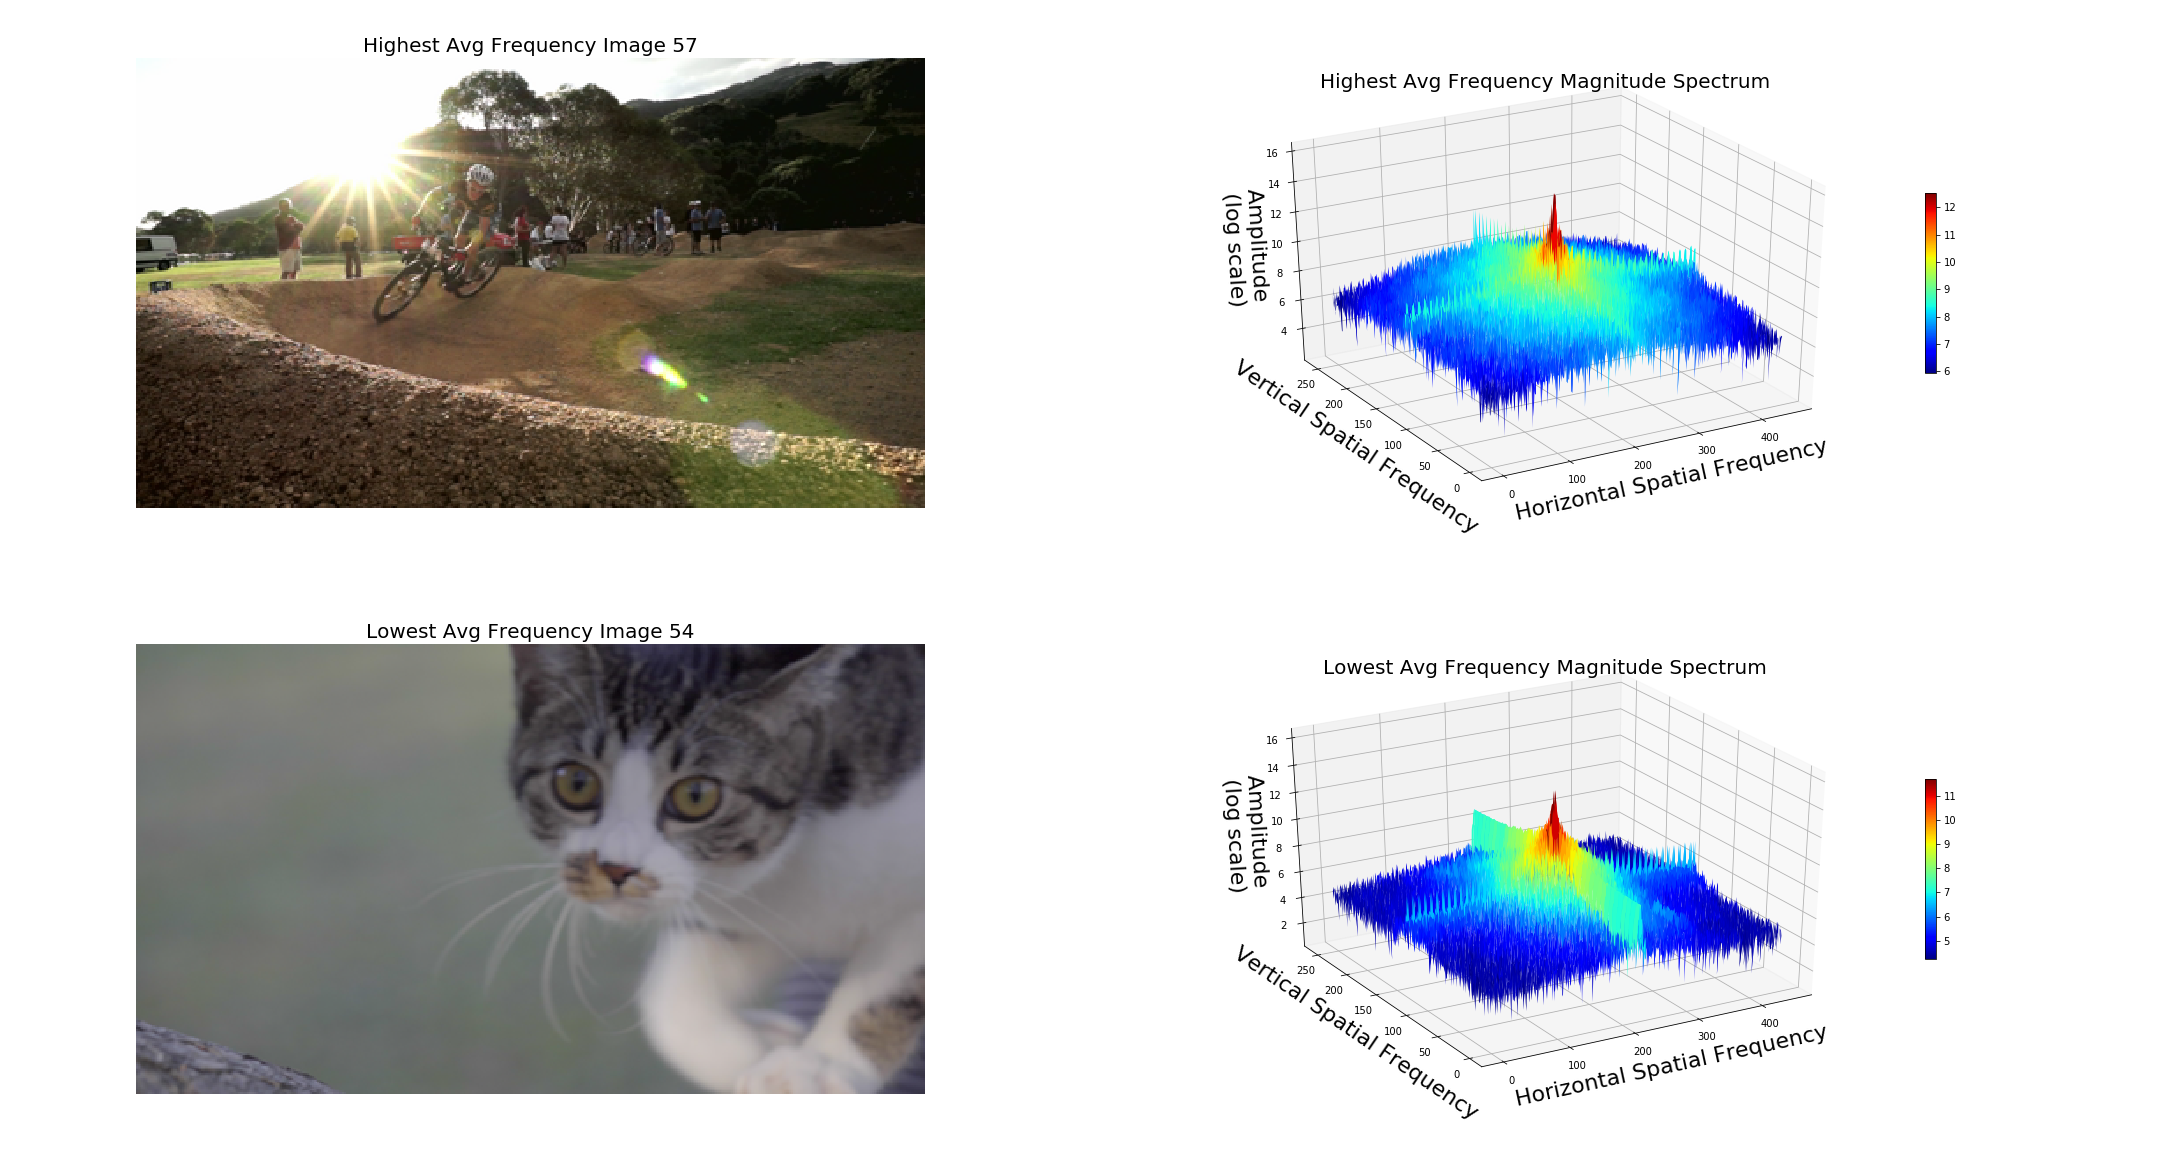
\includegraphics[width=\linewidth]{assets/spatial_frequency/video5spatialfreq.png}
    \caption{Highest and Lowest average Spatial Frequency in Video 5}
    \label{fig:spatial-frequency-5}
\end{figure}

In the images presented above, the image with highest average spatial frequency describes a frame that exhibits a higher concentration of high-frequency components, suggesting that it contains numerous fine details, sharp edges, or abrupt transitions in intensity. These characteristics are often found in complex patterns, textures, or scenes with intricate structures. The prominence of high frequencies indicates that the image may have more contrast between adjacent pixels, leading to a rich texture and detail.

Conversely, the image with lowest average spatial frequency describes a frame that has a dominant presence of low-frequency components, implying smoother transitions and fewer abrupt changes in intensity. This typically results in a more uniform and less detailed appearance, with broad, continuous areas of similar intensity. Such images might depict scenes with large homogeneous regions, minimal texture, or softly varying gradients.

By comparing these two images, we gain insight into the different types of content represented in the dataset. The spatial frequency analysis provides a quantitative means of distinguishing between images with varying levels of detail and texture, helping us understand their underlying structural characteristics.
    
    \pagebreak

\section{\MakeUppercase{Implementation Details}}
The project is developed using Python, leveraging PyTorch as the primary deep learning framework. Interactive Python sessions are utilized for testing and rapid prototyping. Jupyter Notebooks are employed for exploratory data analysis and iterative experimentation, allowing for an interactive and visual approach to model development. TensorBoard is used to visualize training metrics and monitor the performance of the \gls{siren} network during training. Visual Studio Code serves as the main \gls{ide} for code writing and debugging.

\subsection{Instrumentation}
    The software and hardware used for this project are listed below: \\
    \begin{table}[H]
        \caption{Instrumentation Table}
        \label{table:instrumentation-table}
        \centering
        \begin{tabular}{|p{0.2\linewidth}|p{0.3\linewidth}|p{0.4\linewidth}|}
            \hline
            \textbf{Requirement} & \textbf{Solution} & \textbf{Reason} \\
            \hline
            High-Performance Computing & NVIDIA RTX 4090 & Overfitting the video to the model \\
            \hline
            Deep Learning Frameworks & PyTorch & Developing and implementing neural network models \\
            \hline
            Development Environment & Visual Studio Code with Notebook extensions & Running and Debugging Code\\
            \hline
            Web Development Tools & \gls{html}, \gls{css}, JavaScript & Creating an interactive platform to deploy the compression model online \\
            \hline
        \end{tabular}
    \end{table}

\subsection{Hardware Specifications}
The project is trained on a system with the following specifications:
    \begin{itemize}
        \item \textbf{CPU:} The system is equipped with a 13th Gen Intel® Core™ i9-13980HX processor, featuring 32 cores with a base clock speed of 2.42 GHz. This provides substantial computational power for training deep learning models.
        \item \textbf{GPU:} The primary \gls{gpu} is an NVIDIA GeForce RTX 4090 Laptop \gls{gpu} with 15.69 \gls{gib} of VRAM, which accelerates the training and inference processes of the \gls{siren} network. This powerful \gls{gpu} is crucial for handling the complex computations required for video compression tasks.
        \item \textbf{Memory:} The system has a total of 98.23 \gls{gib} of RAM, ensuring ample memory for handling large datasets and complex models during training and evaluation.
    \end{itemize}

\subsection{Neural Network Architecture for Audio}
\begin{figure}[H]
    \centering
    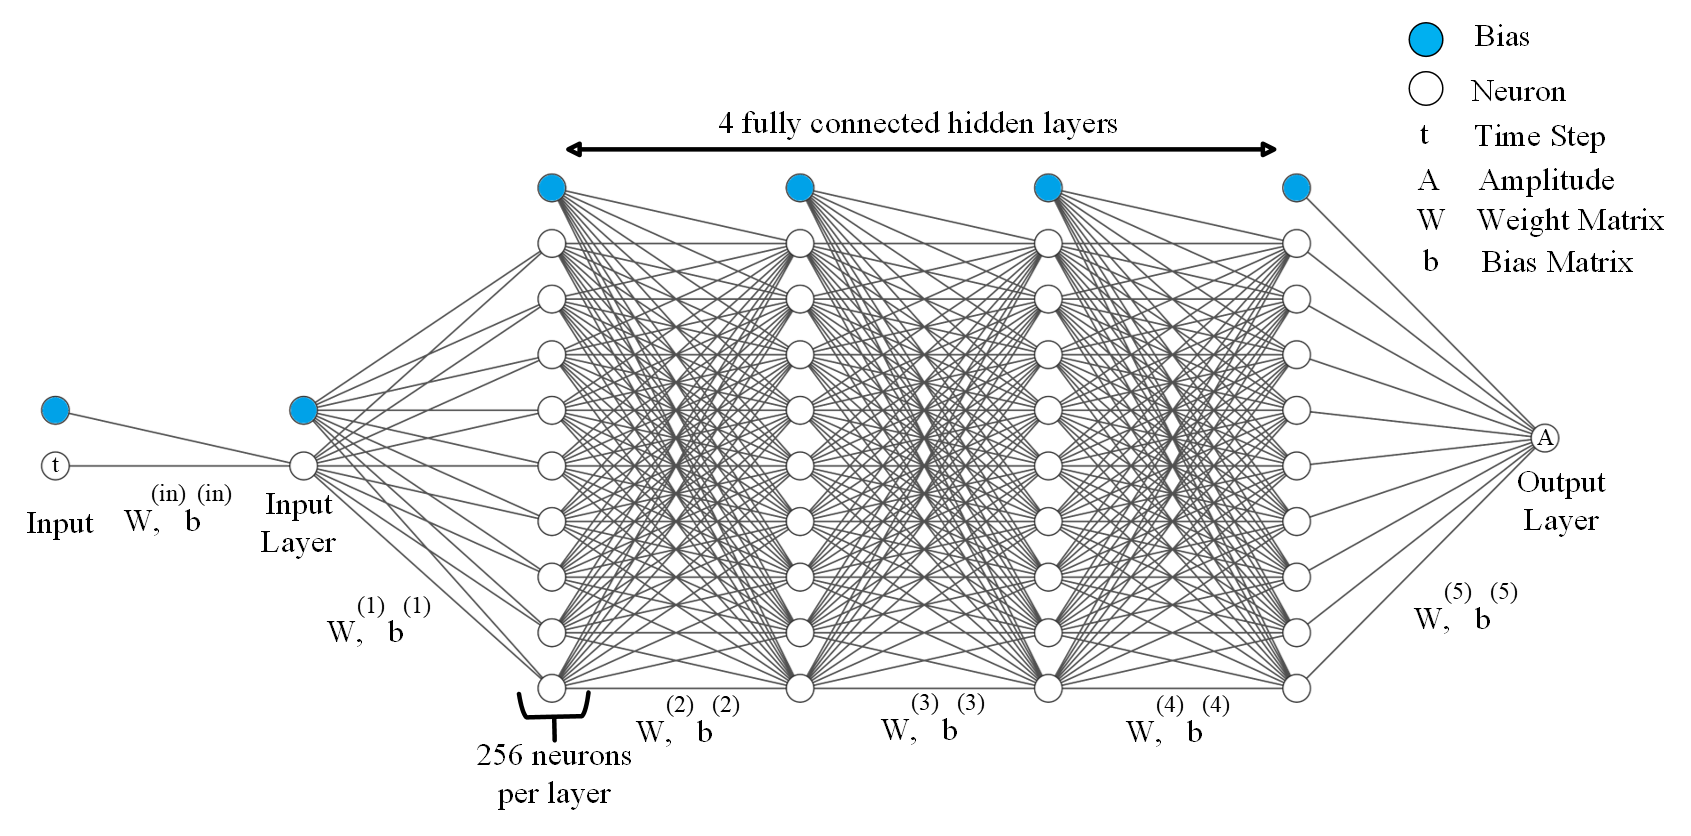
\includegraphics[width=\linewidth]{assets/audio_neural.png}
    \caption{Neural Network Architecture for Audio}
    \label{fig:arch-audio}
\end{figure}
The \gls{siren} model employs a specialized neural network architecture to represent audio signals, as illustrated in \autoref{fig:arch-audio}. This architecture is designed to capture the complex frequency patterns inherent in audio data through a continuous representation.
The network consists of an input layer, four fully connected hidden layers, and an output layer. The input layer accepts a single parameters: time step $(t)$, along with associated input weights $(W_{\text{in}})$ and biases $(b_{\text{in}})$. Each of the four hidden layers comprises 256 neurons, creating a deep structure capable of learning intricate audio features. These hidden layers are fully connected, with each neuron linked to every neuron in the adjacent layers. Each hidden layer is equipped with its own set of weights $(W)$ and biases $(b)$, denoted as $W^{(1)}$, $b^{(1)}$ through $W^{(4)}$, $b^{(4)}$.
The output layer consists of a single neuron, producing the final amplitude value for a given time step. This layer also has its own weights $W^{(5)}$ and biases $b^{(5)}$. A key feature of the this architecture is the use of sinusoidal activation functions between layers, which, although not explicitly shown in the figure, play a crucial role in capturing high-frequency details and periodic patterns typical of audio signals.
This architecture enables the network to learn a continuous representation of audio waveforms as a function of time. By taking time as input and producing amplitude as output, the model can synthesize and manipulate audio at arbitrary temporal resolutions. The depth of the network, combined with the sinusoidal activations, allows for the representation of complex audio features and enables high-quality audio processing tasks.

\subsubsection*{Trainable Parameters}
The dimensions of the trainable parameters (weights and biases) are as follows:

\begin{enumerate}[label=\textbf{\roman*.}]
    \item \textbf{Input to Input Layer}
    \begin{itemize}
        \item Weight matrix \( \mathbf{W}^{(\text{in})} \): \( 1 \times 1 \)
        \item Bias vector \( \mathbf{b}^{(\text{in})} \): \( 1 \)
    \end{itemize}
    \item \textbf{Input Layer to First Hidden Layer}
    \begin{itemize}
        \item Weight matrix \( \mathbf{W}^{(\text{1})} \): \( 1024 \times 1 \)
        \item Bias vector \( \mathbf{b}^{(\text{1})} \): \( 1024 \)
    \end{itemize}
    \item \textbf{Hidden Layers}
    \begin{itemize}
        \item Weight matrices \( \mathbf{W}^{(n)} \) for \( n = 2, 3, 4 \):
        \begin{itemize}
            \item[\(\circ\)] \( \mathbf{W}^{(2)} \): \( 256 \times 256 \)
            \item[\(\circ\)] \( \mathbf{W}^{(3)} \): \( 256 \times 256 \)
            \item[\(\circ\)] \( \mathbf{W}^{(4)} \): \( 256 \times 256 \)
        \end{itemize}
        \item Bias vectors \( \mathbf{b}^{(n)} \) for \( n = 2, 3, 4 \):
        \begin{itemize}
            \item[\(\circ\)] \( \mathbf{b}^{(2)} \): \( 256 \)
            \item[\(\circ\)] \( \mathbf{b}^{(3)} \): \( 256 \)
            \item[\(\circ\)] \( \mathbf{b}^{(4)} \): \( 256 \)
        \end{itemize}
    \end{itemize}
    \item \textbf{Last Hidden Layer to Output Layer}
    \begin{itemize}
        \item Weight matrix \( \mathbf{W}^{(\text{5})} \): \( 1 \times 256 \)
        \item Bias vector \( \mathbf{b}^{(\text{5})} \): \( 1 \)
    \end{itemize}
\end{enumerate}

The total number of trainable parameters in the neural network is 199,683.


\subsection{Neural Network Architecture for Video}
\begin{figure}[H]
    \centering
    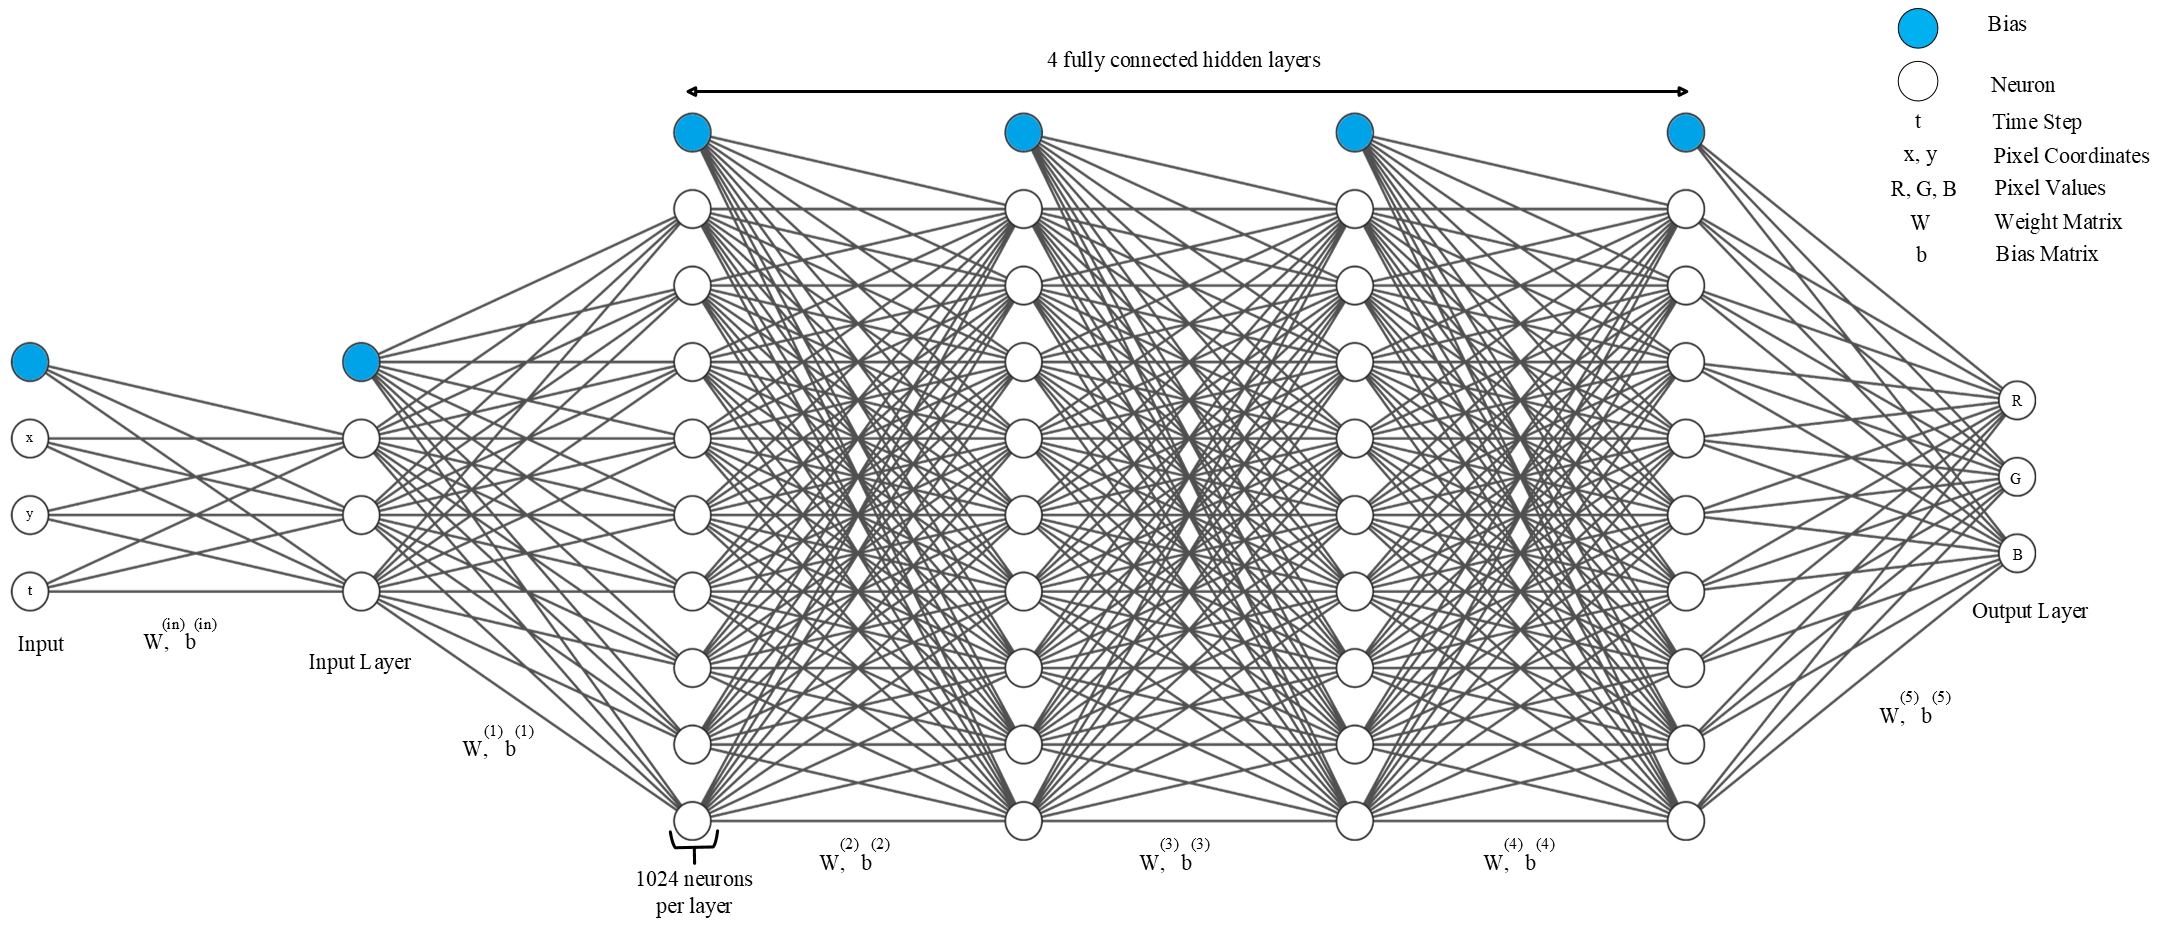
\includegraphics[width=\linewidth]{assets/video_neural.png}
    \caption{Neural Network Architecture for Video}
    \label{fig:arch-video}
\end{figure}

The neural network architecture designed for Implicit Neural Representation for Videos using \gls{siren} is composed as follows:

\begin{itemize}
    \item \textbf{Input Layer}: This layer has 3 neurons, corresponding to the pixel coordinates \( (x, y) \) and the frame index \( t \).
    \item \textbf{Hidden Layers}: There are 4 fully connected hidden layers, each with 1024 neurons. Each hidden layer has its own weight and bias matrix, denoted by \(W\) and \(b\), respectively. These layers utilize the sine activation function, which is pivotal in capturing the dynamic spatial frequency ranges of the video.
    \item \textbf{Output Layer}: This layer contains 3 neurons, producing the RGB values at the specified coordinate and frame.
\end{itemize}

The sine activation function employed in all layers except the output layer allows the network to effectively encapsulate the intricate details of the video's spatial and temporal variations within the weights and biases of the network. This results in a faithful representation of the video content.

\subsubsection*{Trainable Parameters}
The dimensions of the trainable parameters (weights and biases) are as follows:

\begin{enumerate}[label=\textbf{\roman*.}]
    \item \textbf{Input to Input Layer}
    \begin{itemize}
        \item Weight matrix \( \mathbf{W}^{(\text{in})} \): \( 3 \times 3 \)
        \item Bias vector \( \mathbf{b}^{(\text{in})} \): \( 3 \)
    \end{itemize}
    \item \textbf{Input Layer to First Hidden Layer}
    \begin{itemize}
        \item Weight matrix \( \mathbf{W}^{(\text{1})} \): \( 1024 \times 3 \)
        \item Bias vector \( \mathbf{b}^{(\text{1})} \): \( 1024 \)
    \end{itemize}
    \item \textbf{Hidden Layers}
    \begin{itemize}
        \item Weight matrices \( \mathbf{W}^{(n)} \) for \( n = 2, 3, 4 \):
        \begin{itemize}
            \item[\(\circ\)] \( \mathbf{W}^{(2)} \): \( 1024 \times 1024 \)
            \item[\(\circ\)] \( \mathbf{W}^{(3)} \): \( 1024 \times 1024 \)
            \item[\(\circ\)] \( \mathbf{W}^{(4)} \): \( 1024 \times 1024 \)
        \end{itemize}
        \item Bias vectors \( \mathbf{b}^{(n)} \) for \( n = 2, 3, 4 \):
        \begin{itemize}
            \item[\(\circ\)] \( \mathbf{b}^{(2)} \): \( 1024 \)
            \item[\(\circ\)] \( \mathbf{b}^{(3)} \): \( 1024 \)
            \item[\(\circ\)] \( \mathbf{b}^{(4)} \): \( 1024 \)
        \end{itemize}
    \end{itemize}
    \item \textbf{Last Hidden Layer to Output Layer}
    \begin{itemize}
        \item Weight matrix \( \mathbf{W}^{(\text{5})} \): \( 3 \times 1024 \)
        \item Bias vector \( \mathbf{b}^{(\text{5})} \): \( 3 \)
    \end{itemize}
\end{enumerate}

The total number of trainable parameters in the neural network is 3,155,983.

\subsection{Hyperparameters}
 Below is a table summarizing the key hyperparameters used in our model:

% \begin{table}[H]
% \caption{Hyperparameters Used in Models}
% \centering
% \begin{tabular}{|c|c|p{7cm}|}
% \hline
% \textbf{Hyperparameter} & \textbf{Value} & \textbf{Description} \\
% \hline
% Learning Rate & \( 1 \times 10^{-4} \) & Controls the step size at each iteration while moving toward a minimum of the loss function. \\
% \hline
% Batch Size & 1 & Number of samples processed before the model is updated. \\
% \hline
% \( \omega_0 \) & 30 & Initial value for the first layer's weights, ensuring the sine function spans multiple periods over \([-1, 1]\). \\
% \hline
% Sample Fraction & \([0.5, 0.05,0.01,0.005]\) & Fraction of video pixels to sample in each batch. \\
% \hline
% Epochs & \([1000, 2000,3000, 1500]\) & Number of complete passes through the training dataset. \\
% \hline
% \end{tabular}
% \label{tab:hyperparameters}
% \end{table}

\begin{table}[H]
    \caption{Hyperparameters Used in Models}
    \centering
    \begin{tabular}{|c|p{11cm}|}
    \hline
    \textbf{Hyperparameter} & \textbf{Description} \\
    \hline
    Learning Rate & Controls the step size at each iteration while moving toward a minimum of the loss function. \\
    \hline
    Batch Size & Number of samples processed before the model is updated. \\
    \hline
    \( \omega_0 \) & Initial value for the first layer's weights, ensuring the sine function spans multiple periods over \([-1, 1]\). \\
    \hline
    Sample Fraction & Fraction of video pixels to sample in each batch. \\
    \hline
    Epochs & Number of complete passes through the training dataset. \\
    \hline
    \end{tabular}
    \label{tab:hyperparameters-description}
\end{table}

\begin{table}[H]
    \caption{Hyperparameters for Audio}
    \centering
    \begin{tabular}{|c|c|}
    \hline
    \textbf{Hyperparameter} & \textbf{Values} \\
    \hline
    Learning Rate & \( 1 \times 10^{-4} \) \\
    \hline
    Batch Size & 1 \\
    \hline
    Epochs & 1000 \\
    \hline
    \( \omega_0 \) & 30 \\
    \hline
    \end{tabular}
    \label{tab:hyperparameters-audio}
\end{table}



\begin{table}[H]
    \caption{Hyperparameters for Different Video Types}
    \centering
    \begin{tabular}{|c|c|c|c|c|c|}
    \hline
    \textbf{Video Name} & \textbf{Batch Size} & \textbf{Learning Rate} & \textbf{\( \omega_0 \)} & \textbf{Epochs} & \textbf{Sample Fraction} \\
    \hline
    Very Very Short & 1 & \( 1 \times 10^{-4} \) & 30 & 1000 & 0.5 \\
    \hline
    Very Short & 1 & \( 1 \times 10^{-4} \) & 30 & 3000 & 0.5 \\
    \hline
    Short & 1 & \( 1 \times 10^{-4} \) & 30 & 2000 & 0.05 \\
    \hline
    Medium & 1 & \( 1 \times 10^{-4} \) & 30 & 2000 & 0.01 \\
    \hline
    Long & 1 & \( 1 \times 10^{-4} \) & 30 & 1500 & 0.005 \\
    \hline
    \end{tabular}
    \label{tab:hyperparameters-video}
\end{table}



\pagebreak 

\section{\MakeUppercase{Results and Analysis}}

    
    \subsection{Audio Dataset}
    This section presents two visualizations of the audio signal: the first subplot shows amplitude over time with notable peaks, and the second subplot is a spectrogram displaying frequency content and amplitude intensity. Additionally, a table provides \gls{psnr} and log spectral distance metrics for ground truth and prediction pairs, assessing signal fidelity and frequency representation accuracy.
    
    \begin{figure}[H]
        \centering
        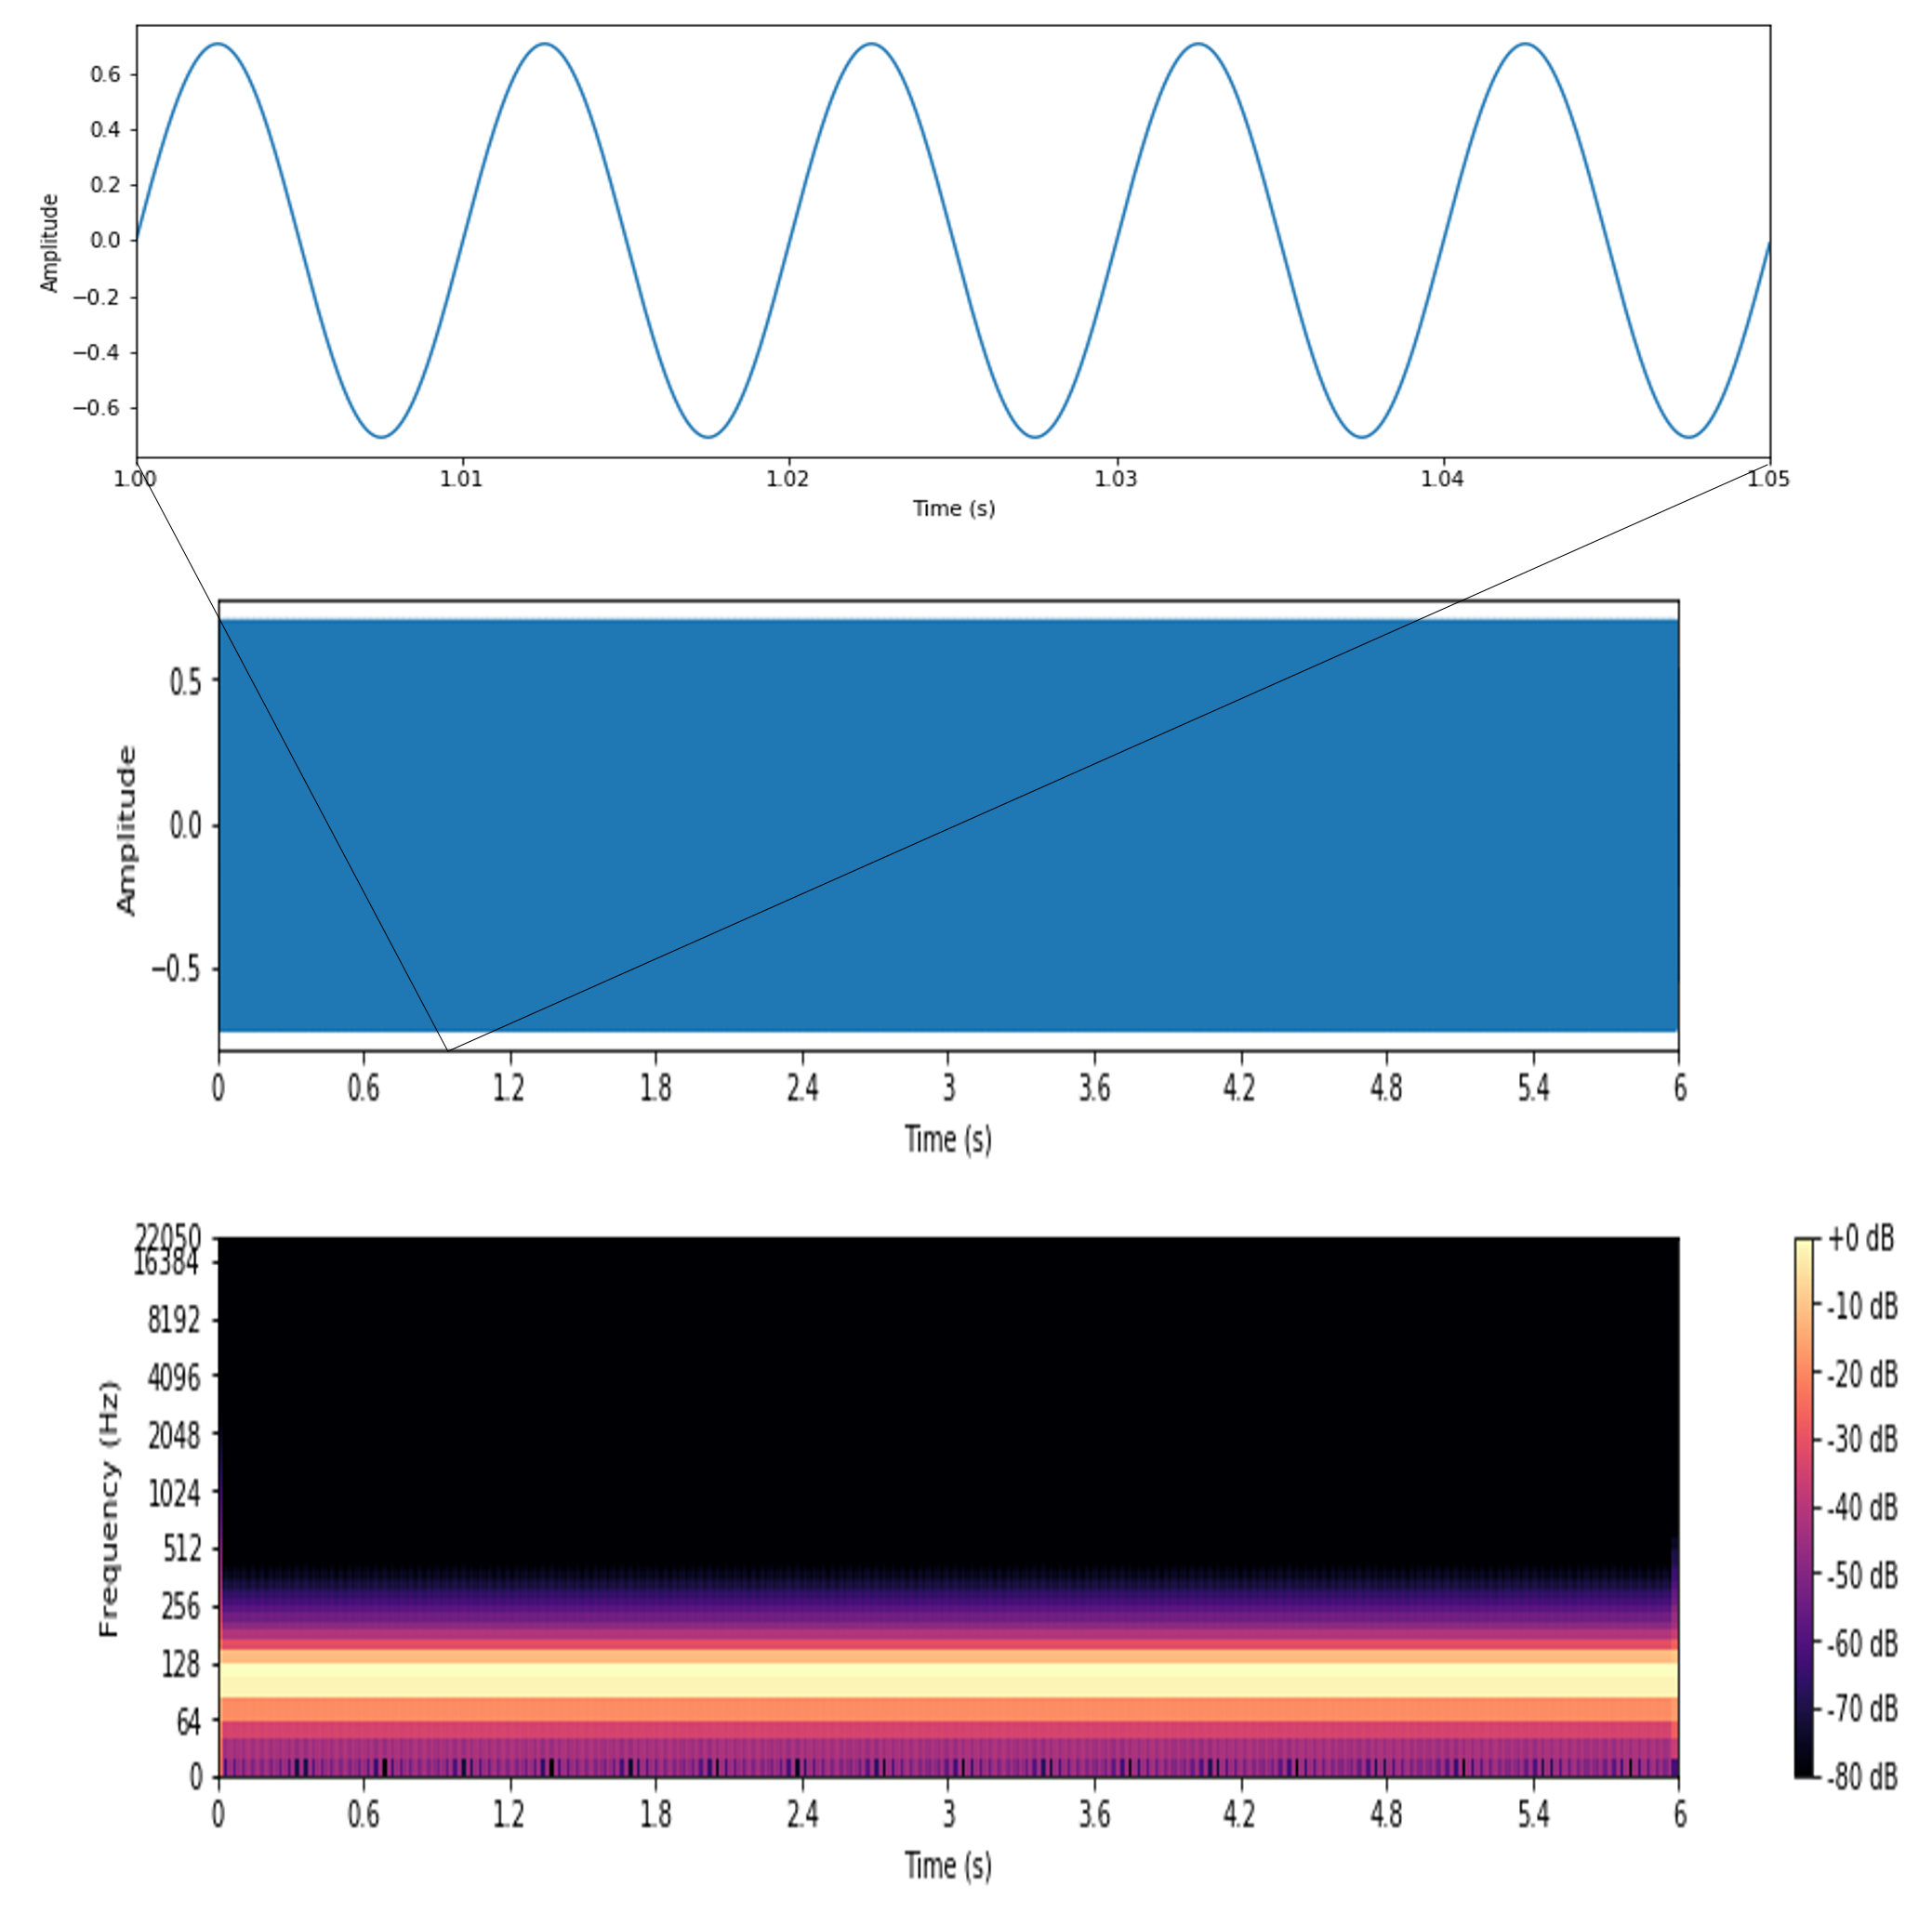
\includegraphics[width=\linewidth]{assets/audio_results/puretone100hz.png}
        \caption{Spectogram of Ground Truth Puretone 100Hz Audio}
        \label{fig:gt-pure100-spec}
    \end{figure}
    
    \begin{figure}[H]
        \centering
        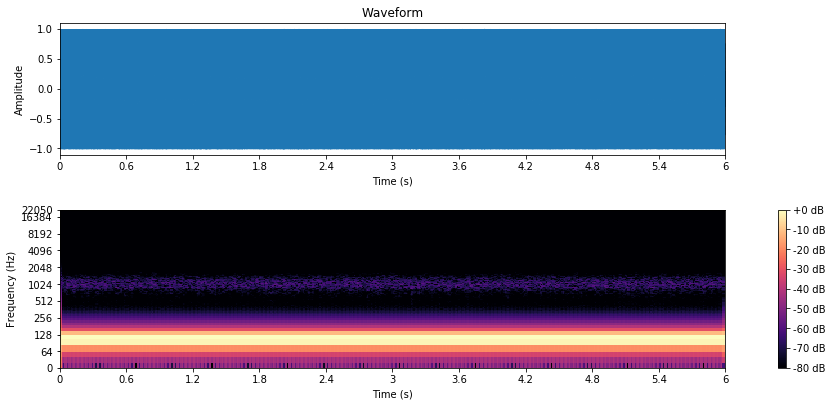
\includegraphics[width=\linewidth]{assets/audio_results/puretone100hzpred.png}
        \caption{Spectogram of Predicted Puretone 100Hz Audio}
        \label{fig:pred-pure100-spec}
    \end{figure}

     \begin{figure}[H]
        \centering
        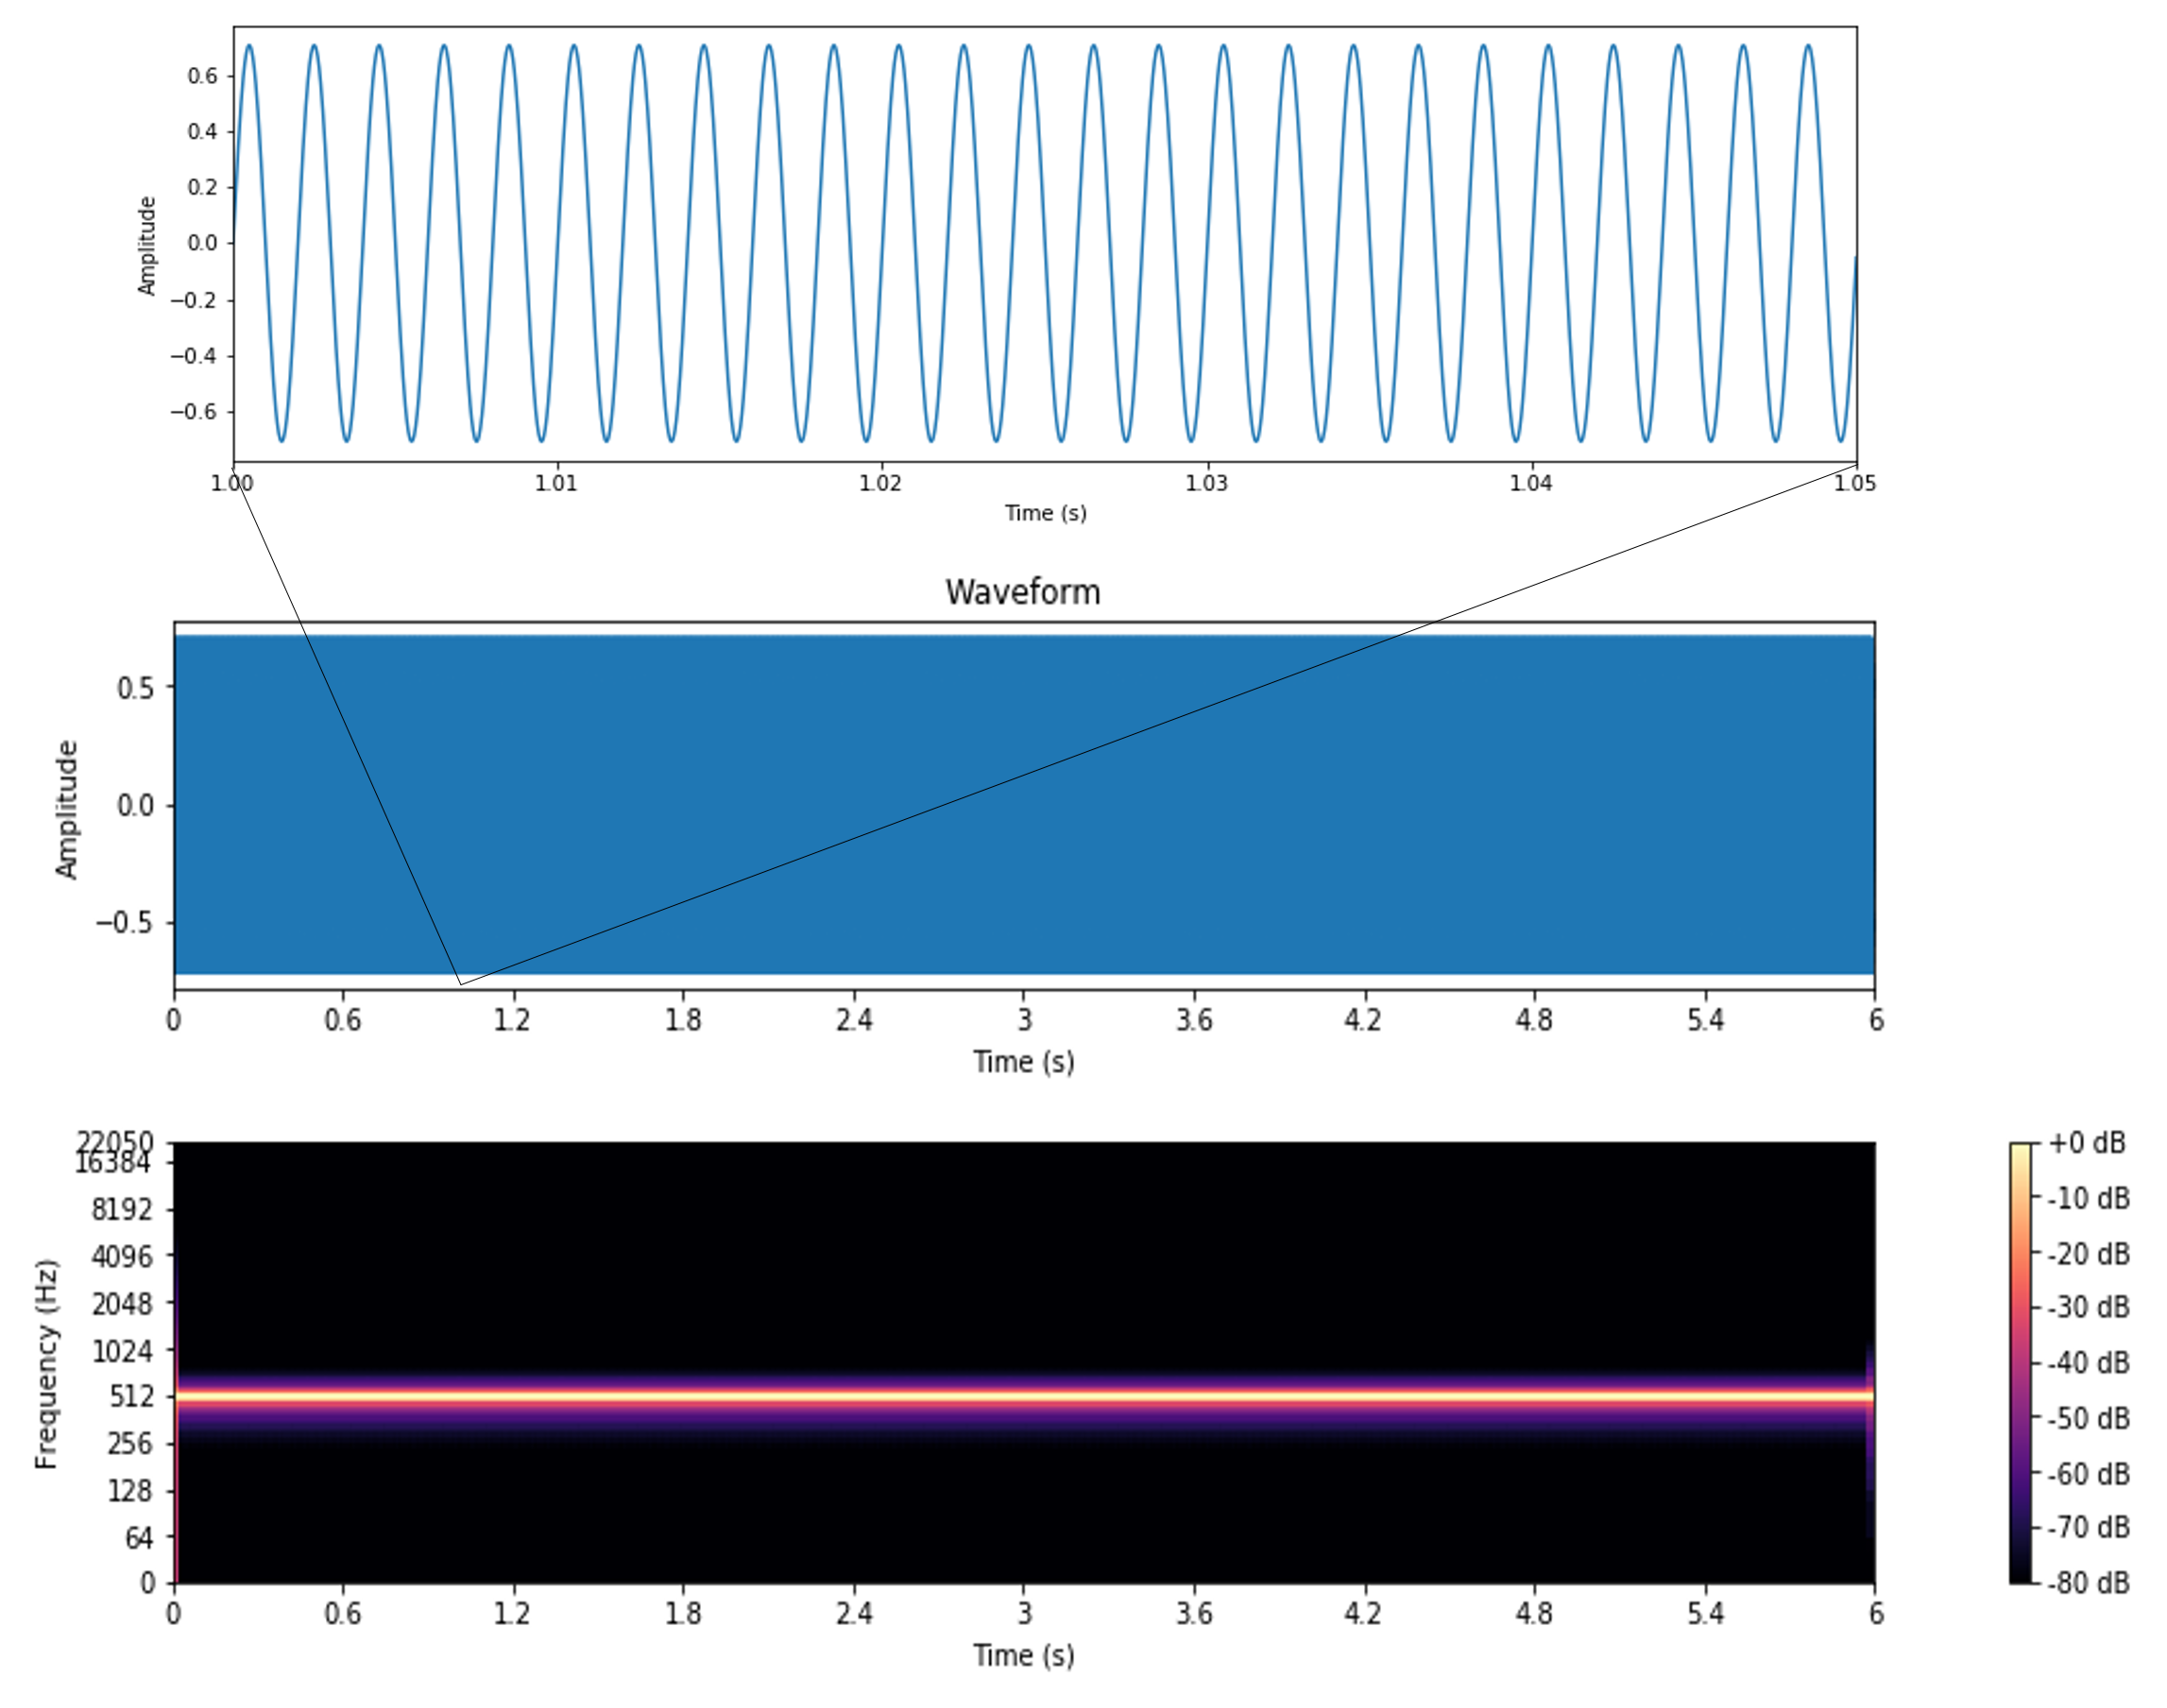
\includegraphics[width=\linewidth]{assets/audio_results/puretone500hz.png}
        \caption{Spectogram of Ground Truth Puretone 500Hz Audio}
        \label{fig:gt-pure500-spec}
    \end{figure}
    
    \begin{figure}[H]
        \centering
        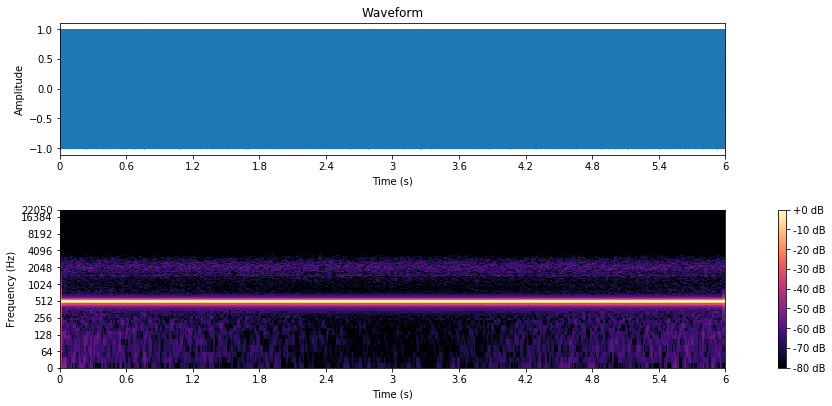
\includegraphics[width=\linewidth]{assets/audio_results/puretone500hzpred.png}
        \caption{Spectogram of Predicted Puretone 500Hz Audio}
        \label{fig:pred-pure500-spec}
    \end{figure}

    \begin{figure}[H]
        \centering
        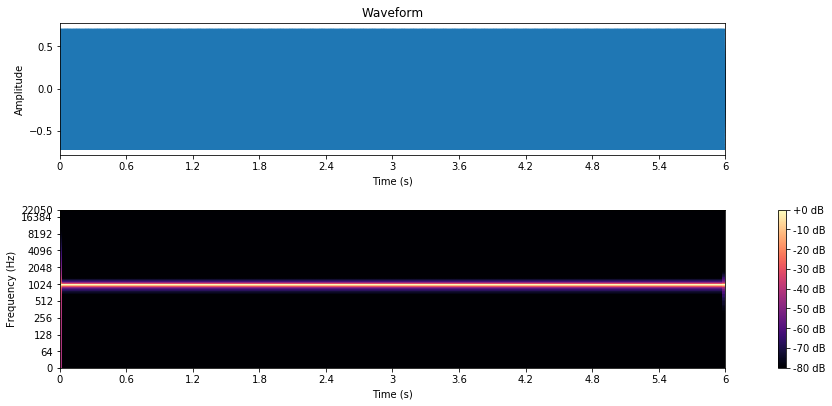
\includegraphics[width=\linewidth]{assets/audio_results/puretone1000hz.png}
        \caption{Spectogram of Ground Truth Puretone 1000Hz Audio}
        \label{fig:gt-pure1000-spec}
    \end{figure}
    
    \begin{figure}[H]
        \centering
        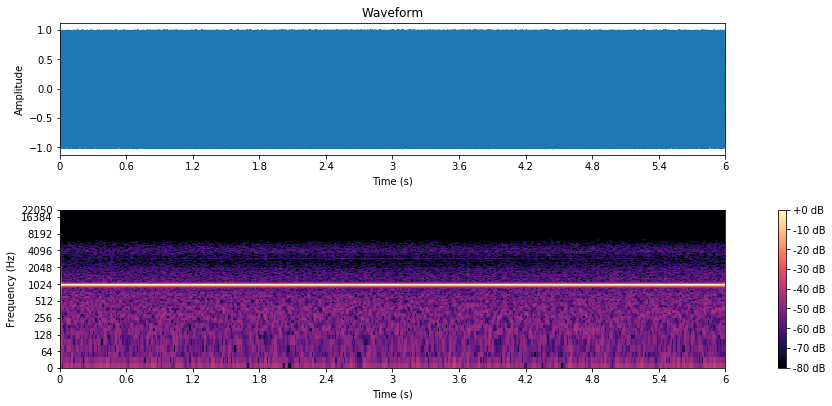
\includegraphics[width=\linewidth]{assets/audio_results/puretone1000hzpred.png}
        \caption{Spectogram of Predicted Puretone 1000Hz Audio}
        \label{fig:pred-pure1000-spec}
    \end{figure}


    
    The spectrograms provided offer a detailed comparison between the ground truth and predicted audio signals for pure tones at 100 Hz, 500 Hz, and 1000 Hz, highlighting key differences in signal quality and noise levels. In the ground truth spectrograms, the audio signals are represented by clear, strong lines at the respective frequencies, with consistent amplitude and minimal noise throughout the 6-second duration. Specifically, the 100 Hz and 500 Hz tones are depicted by bright horizontal lines at their respective frequencies, indicating robust and uniform signals. The 1000 Hz tone similarly shows a strong, well-defined line, demonstrating a consistent and clean signal.

    In contrast, the predicted spectrograms, while correctly identifying the fundamental frequencies, exhibit more noise and reduced signal intensity. The 100 Hz and 5000 Hz predicted tones display additional noise also as the frequency increases, the amount of noise also increases, which is seen from the noisier representations of the higher frequency tones. The predicted 1000 Hz tone shows even more noise and diminished clarity and intensity compared to its ground truth counterpart. While the primary frequency band around 1000 Hz is present, there are additional frequency components and higher intensity variations that are not present in the ground truth. These discrepancies suggest that the model introduced extra harmonics and fluctuations, leading to a less accurate and more distorted representation of the original signals. 

    \begin{figure}[H]
        \centering
        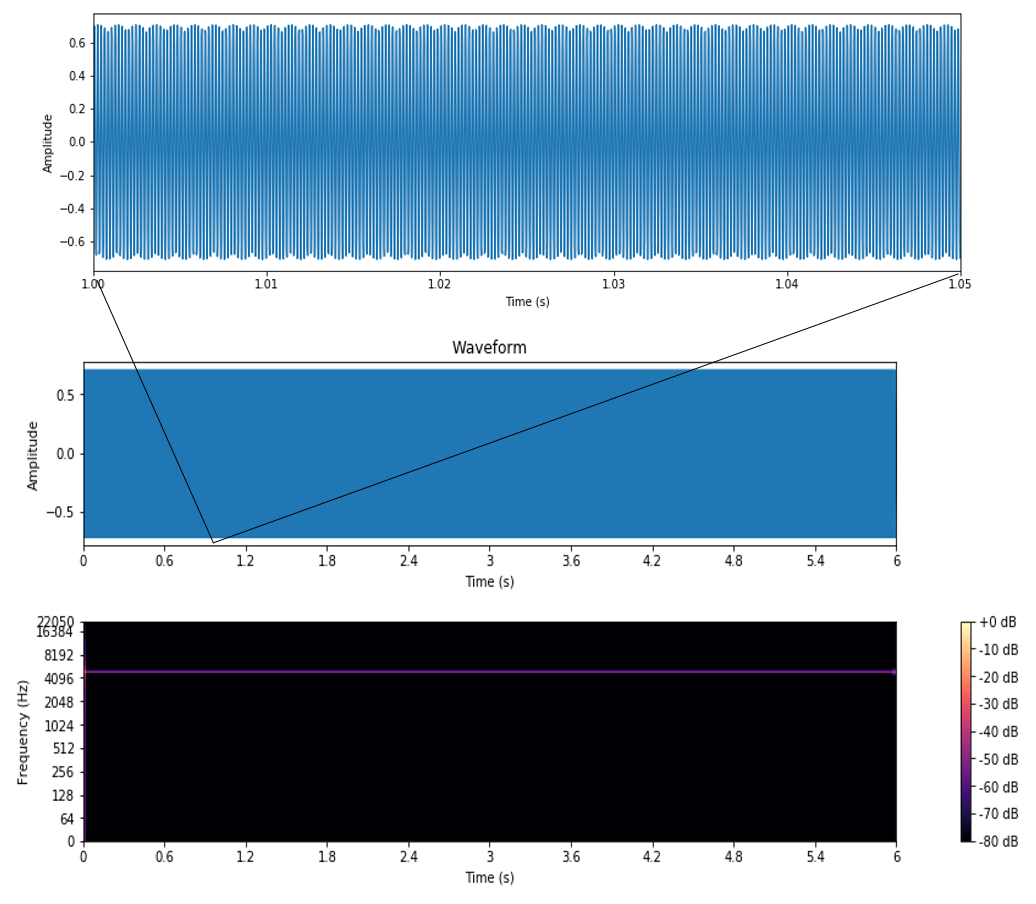
\includegraphics[width=\linewidth]{assets/audio_results/puretone5000hz.png}
        \caption{Spectogram of Ground Truth Puretone 5000Hz Audio}
        \label{fig:gt-pure5000-spec}
    \end{figure}
    
    \begin{figure}[H]
        \centering
        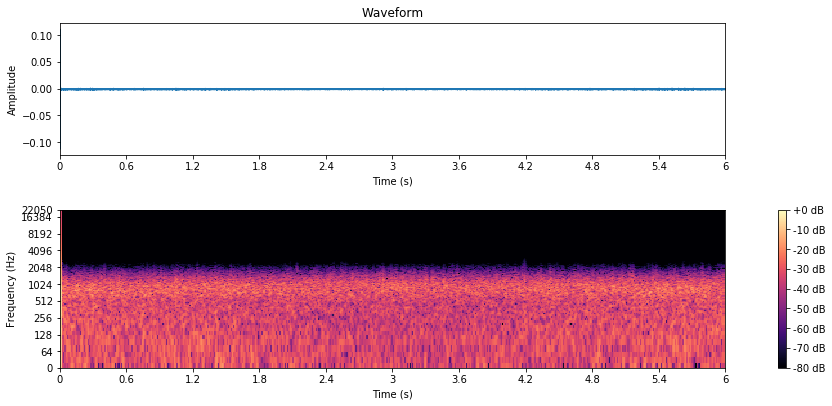
\includegraphics[width=\linewidth]{assets/audio_results/puretone5000hzpred.png}
        \caption{Spectogram of Predicted Puretone 5000Hz Audio}
        \label{fig:pred-pure5000-spec}
    \end{figure}

    We observe a clear distinction between the ground truth and predicted pure tone audio at 5000Hz. The ground truth waveform displays an amplitude fluctuating consistently between -1 and +1, indicating a strong and stable signal. In contrast, the predicted waveform exhibits a significantly lower amplitude, fluctuating between approximately -0.1 and +0.1. This predicted waveform is almost flat, indicating the model's inability to accurately generate the desired signal. Furthermore, the frequency vs. time plot for the ground truth audio shows a single, distinct line at 5000Hz, confirming the purity of the tone. However, the plot for the predicted audio reveals additional lower frequency components, suggesting that the model fails to accurately predict the 5000Hz frequency and instead generates noise.

    \begin{figure}[H]
        \centering
        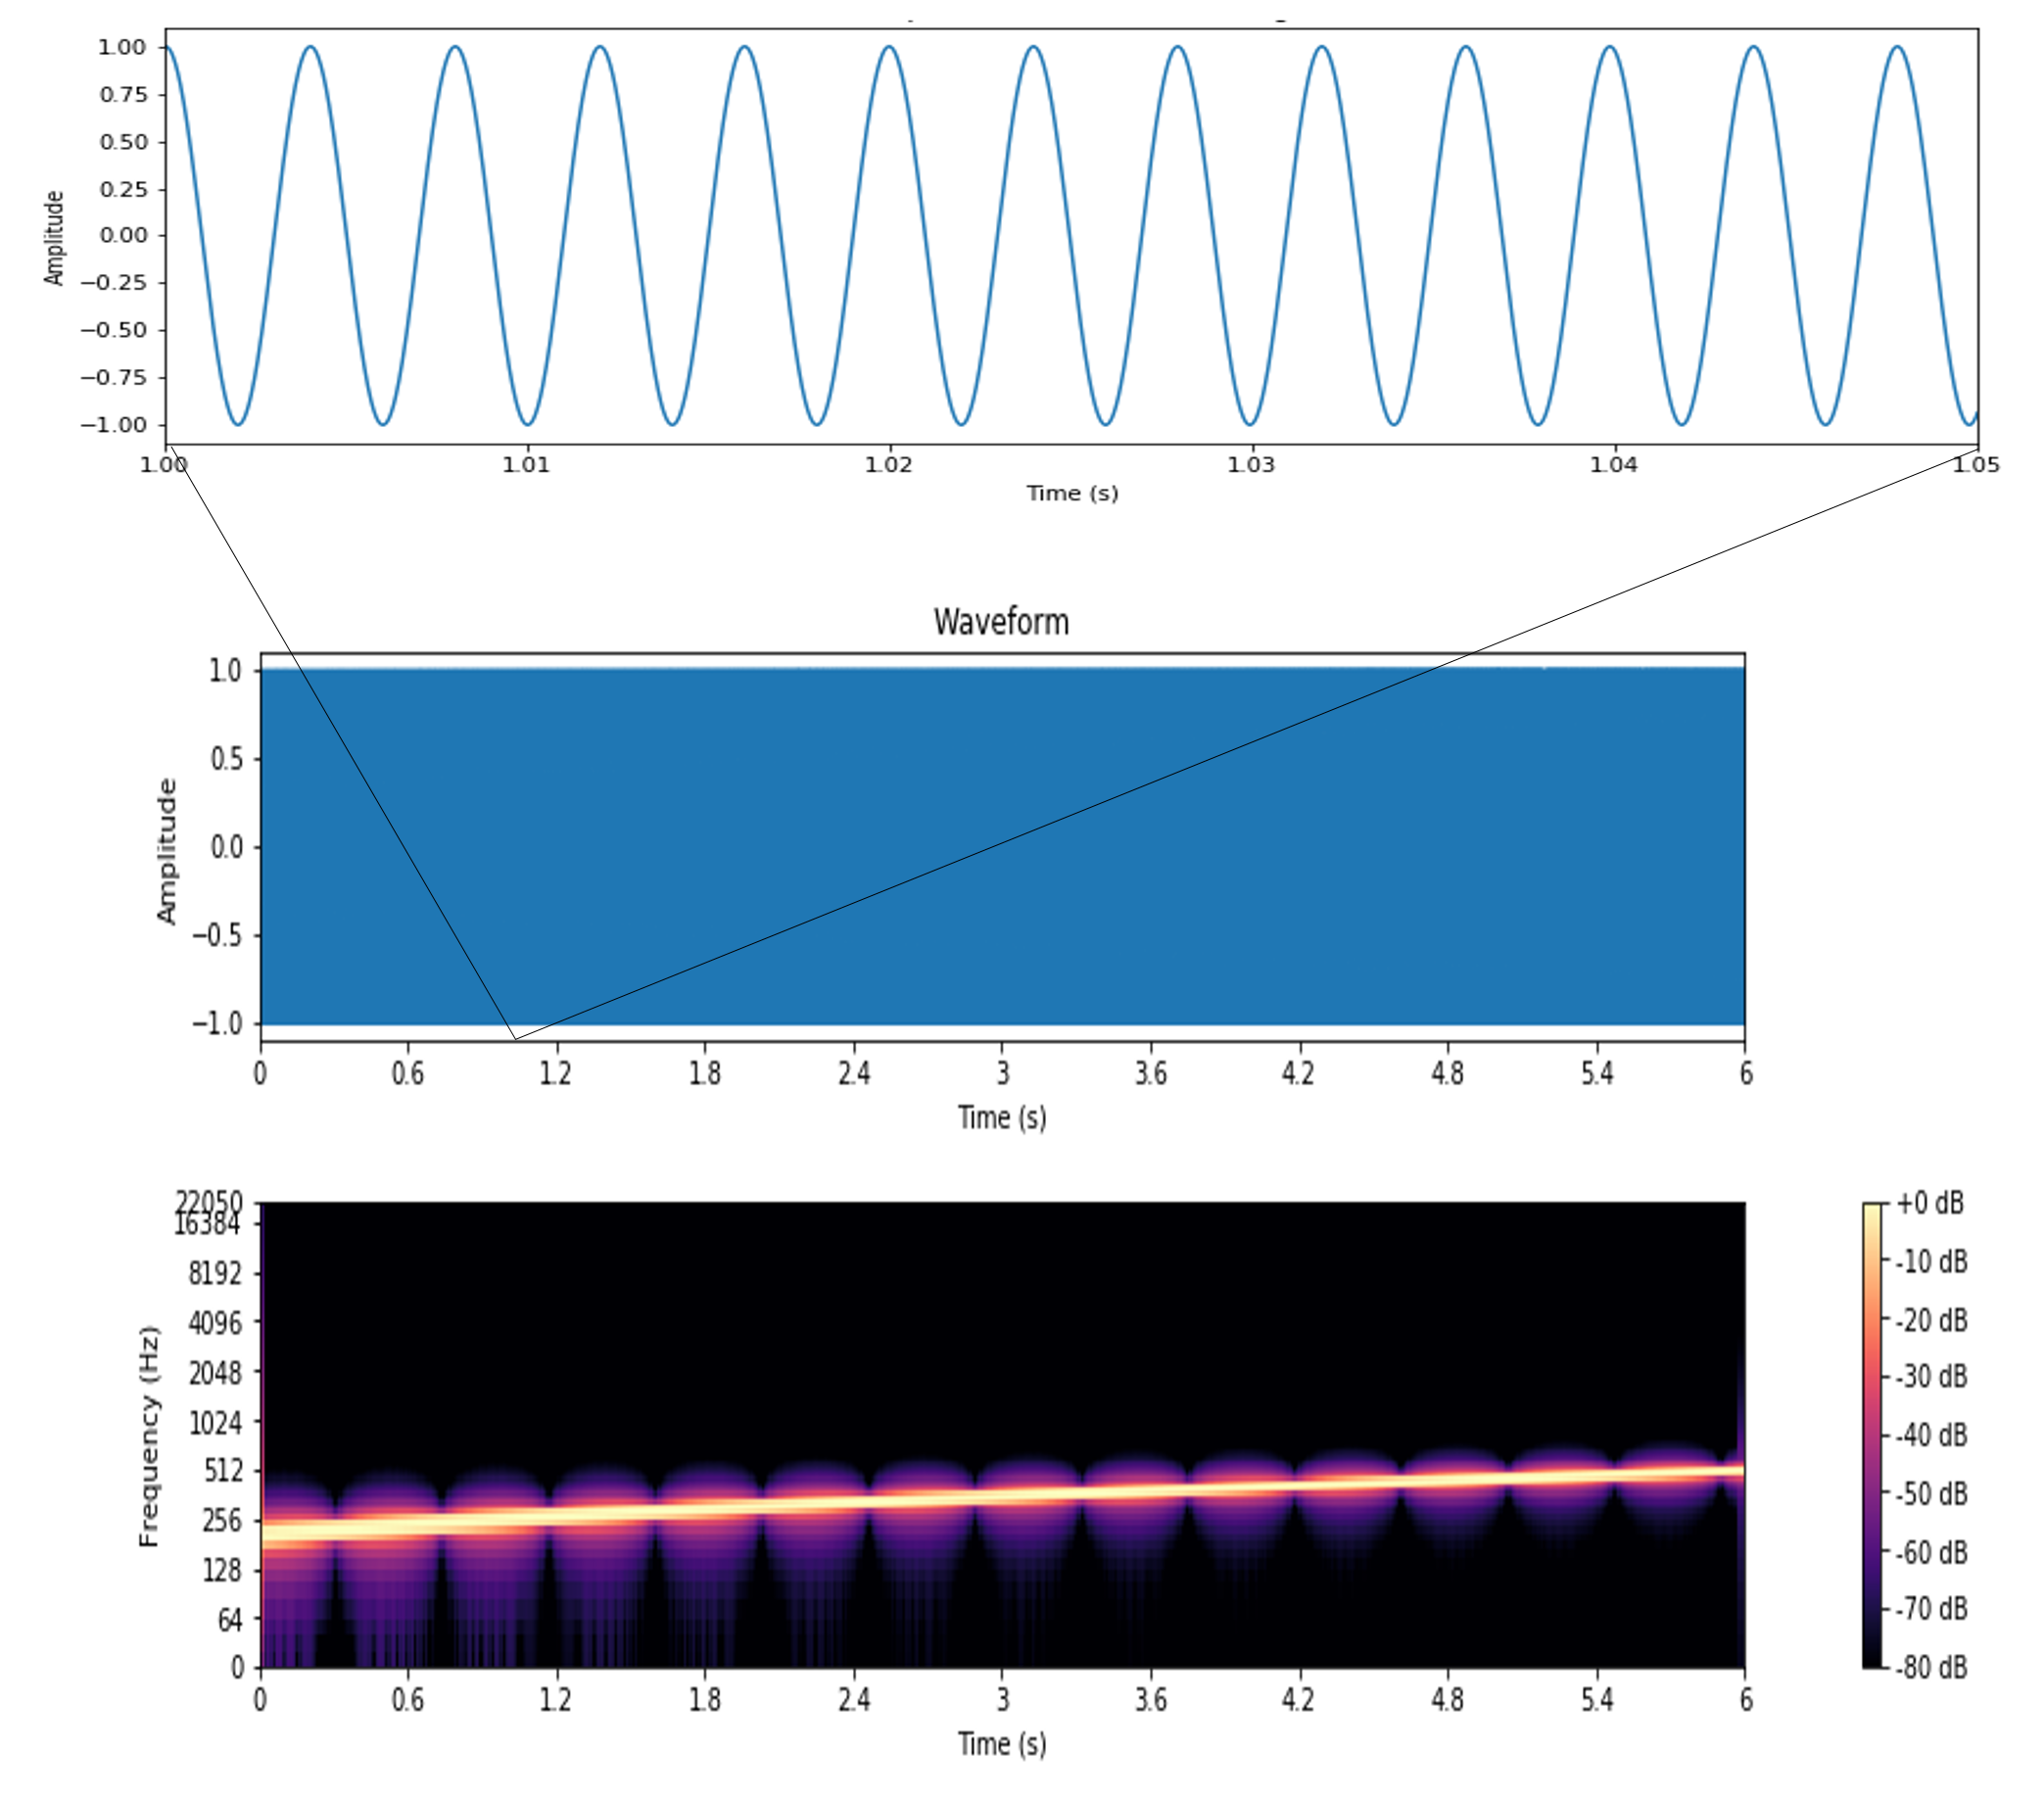
\includegraphics[width=\linewidth]{assets/audio_results/sweeping_tone200-500hz.png}
        \caption{Spectogram of Ground Truth Sweeping Tone 200-500Hz Audio}
        \label{fig:gt-sweep200-500-spec}
    \end{figure}
    
    \begin{figure}[H]
        \centering
        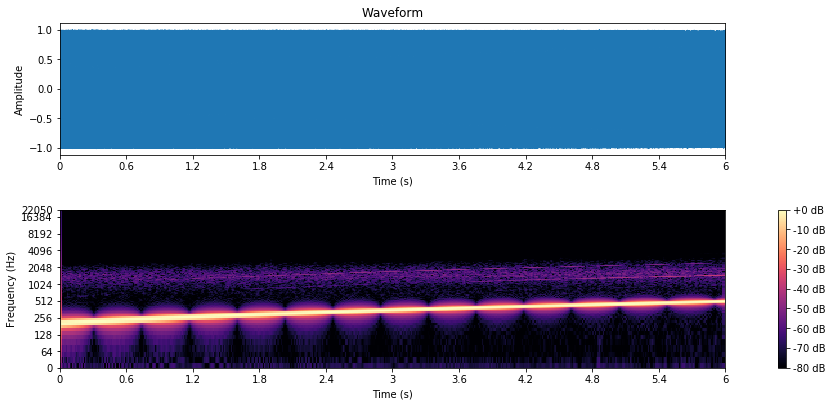
\includegraphics[width=\linewidth]{assets/audio_results/sweeping_tone200-500hzpred.png}
        \caption{Spectogram of Predicted Sweeping Tone 200-500Hz Audio}
        \label{fig:pred-sweep200-500-spec}
    \end{figure}

    \begin{figure}[H]
        \centering
        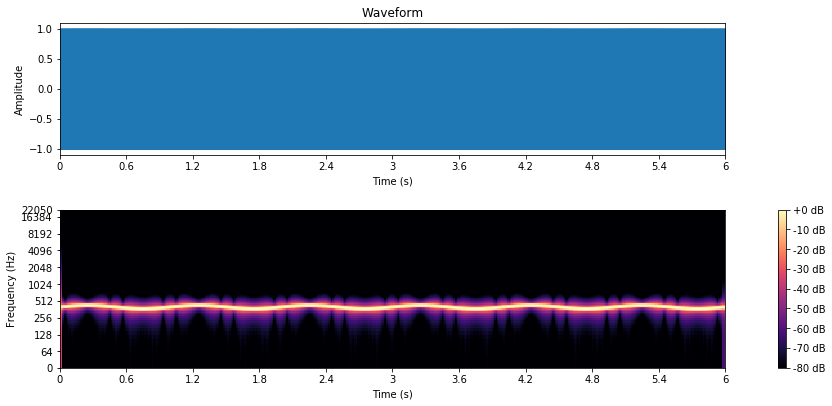
\includegraphics[width=\linewidth]{assets/audio_results/fluctuating_tone400.png}
        \caption{Spectogram of Ground Truth Fluctuating 400Hz Audio}
        \label{fig:gt-fluc400-spec}
    \end{figure}
    
    \begin{figure}[H]
        \centering
        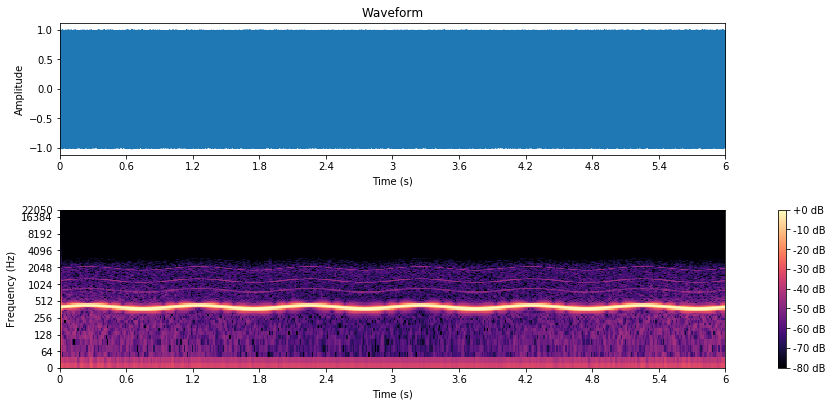
\includegraphics[width=\linewidth]{assets/audio_results/fluctuating_tone400pred.png}
        \caption{Spectogram of Predicted Fluctuating 400Hz Audio}
        \label{fig:pred-fluc400-spec}
    \end{figure}


    \begin{figure}[H]
        \centering
        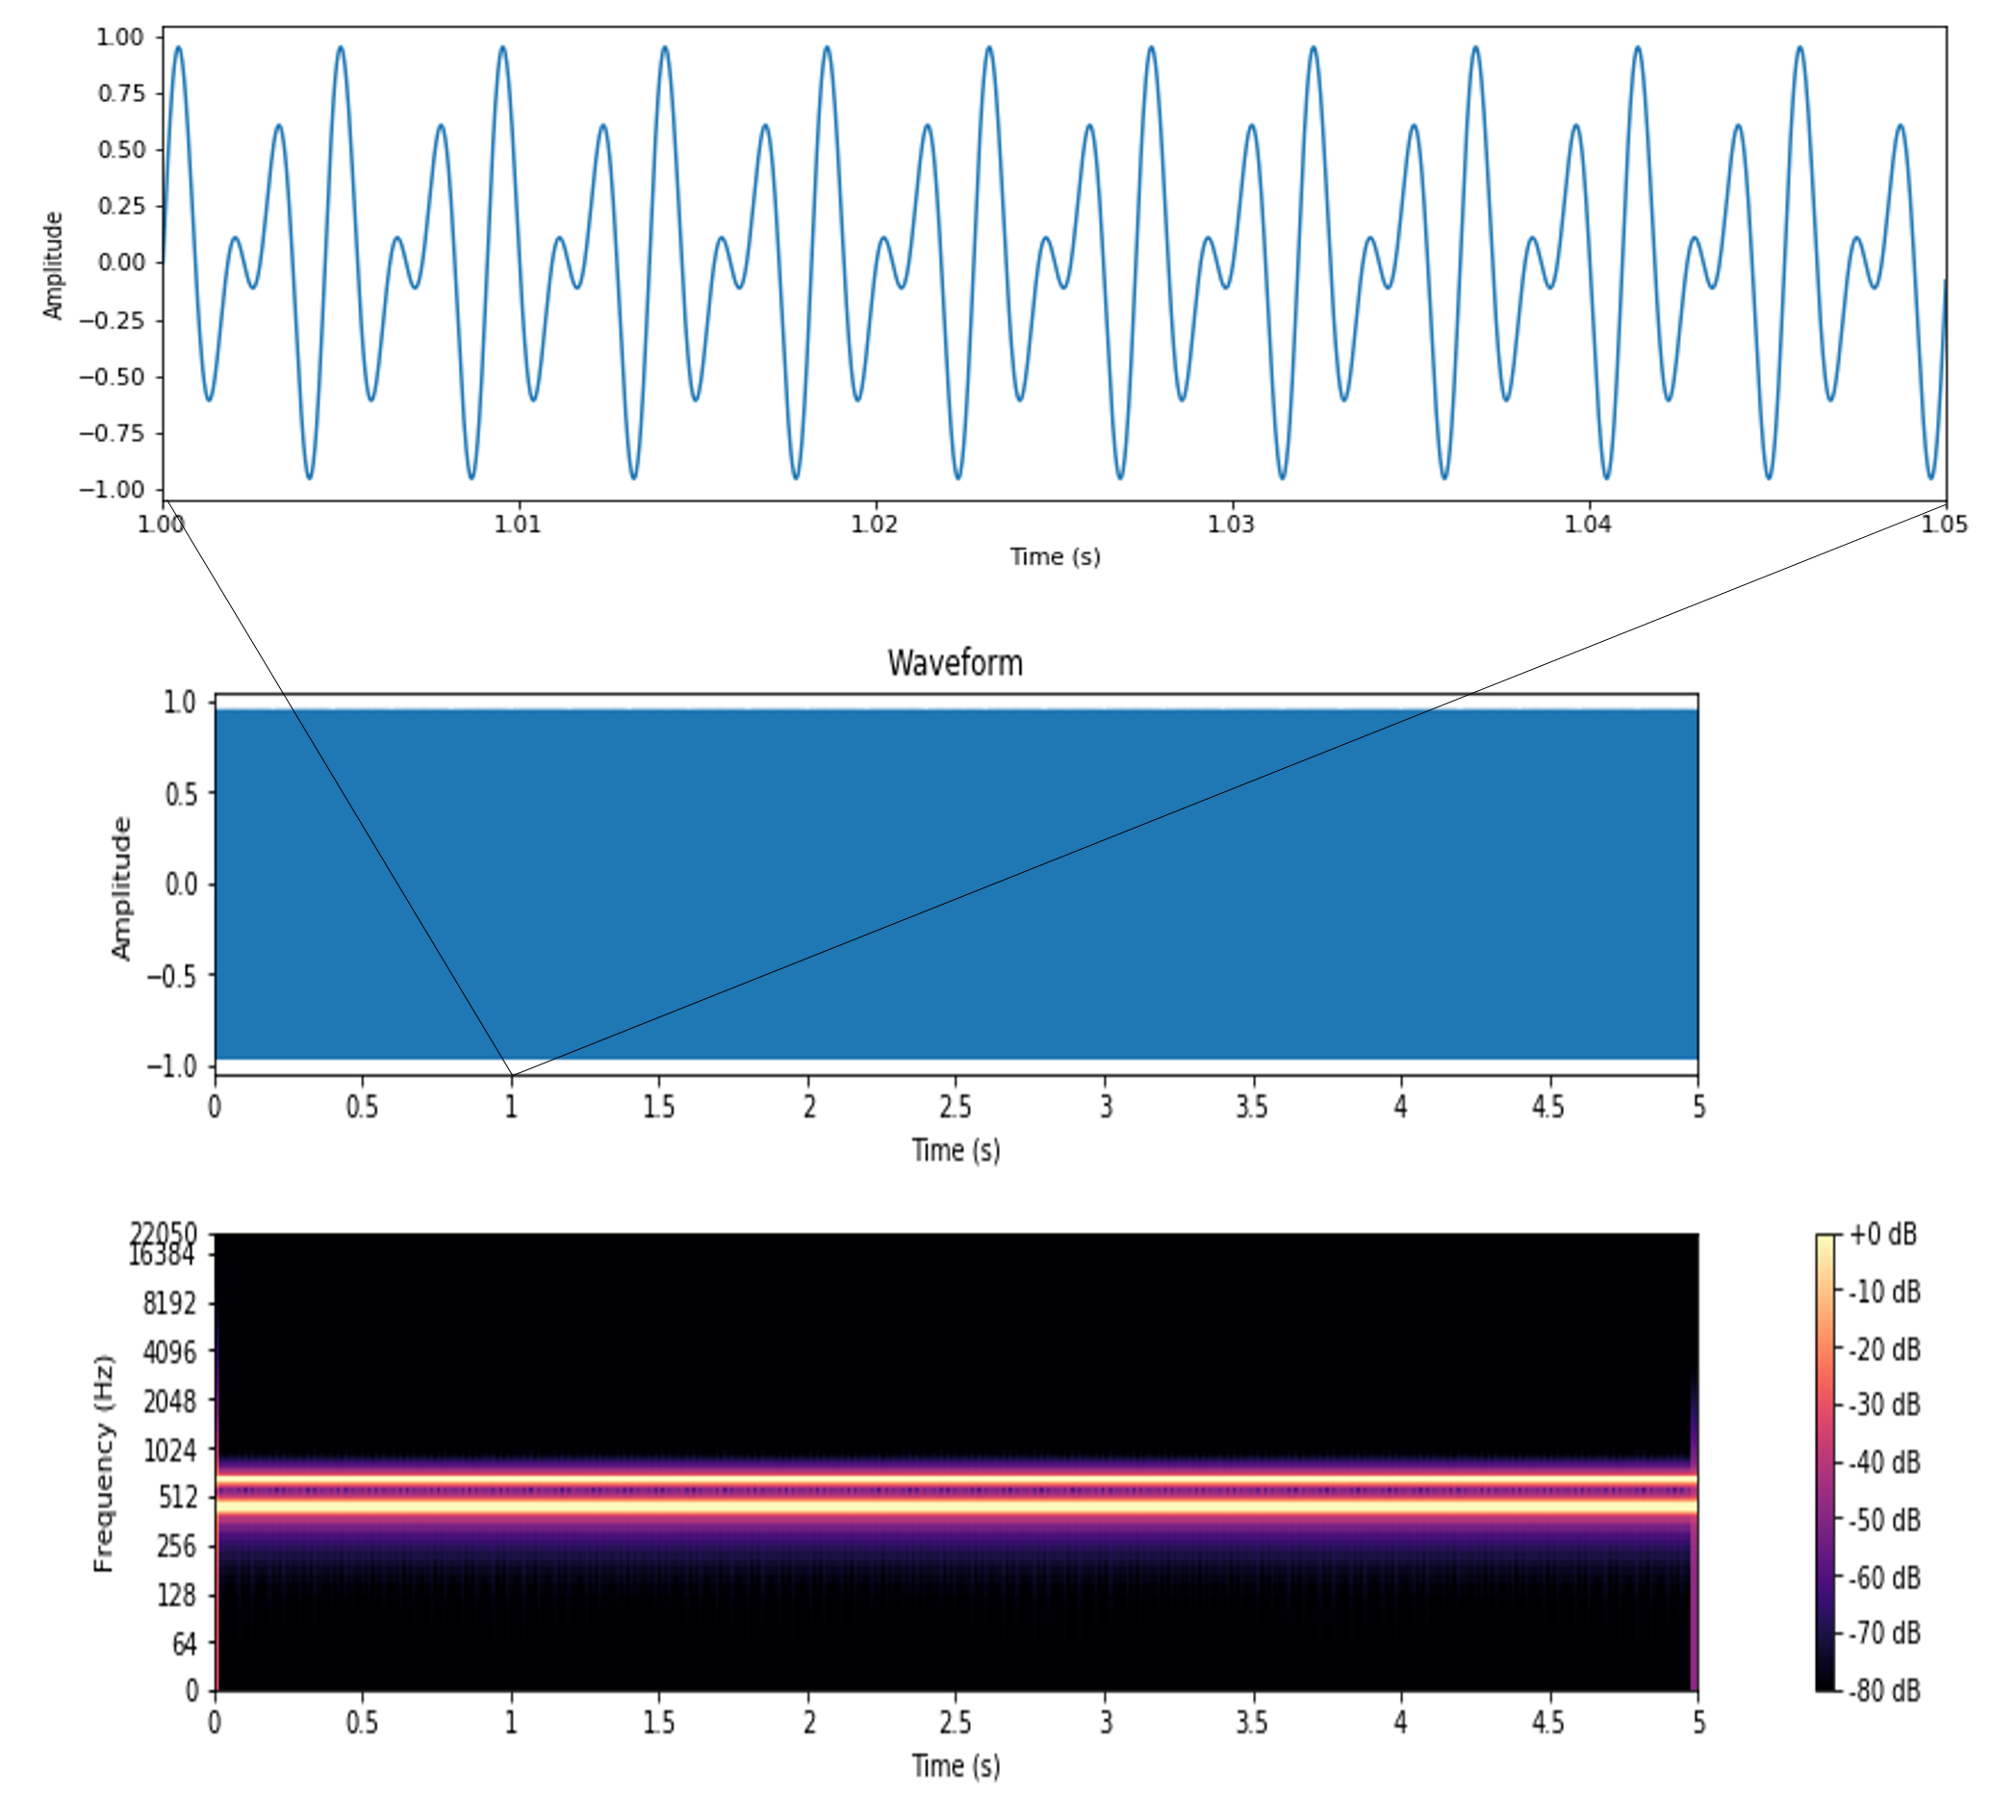
\includegraphics[width=\linewidth]{assets/audio_results/multitoneA4E4.png}
        \caption{Spectogram of Ground Truth Multitone A4E4 audio}
        \label{fig:gt-multiA4E4-spec}
    \end{figure}
    
    \begin{figure}[H]
        \centering
        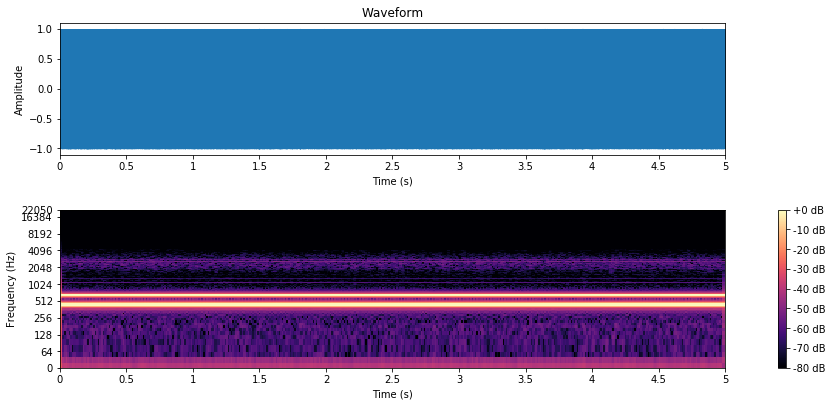
\includegraphics[width=\linewidth]{assets/audio_results/multitoneA4E4pred.png}
        \caption{Spectogram of Predicted Multitone A4E4 Seconds Audio}
        \label{fig:pred-multiA4E4-spec}
    \end{figure}


    \begin{figure}[H]
        \centering
        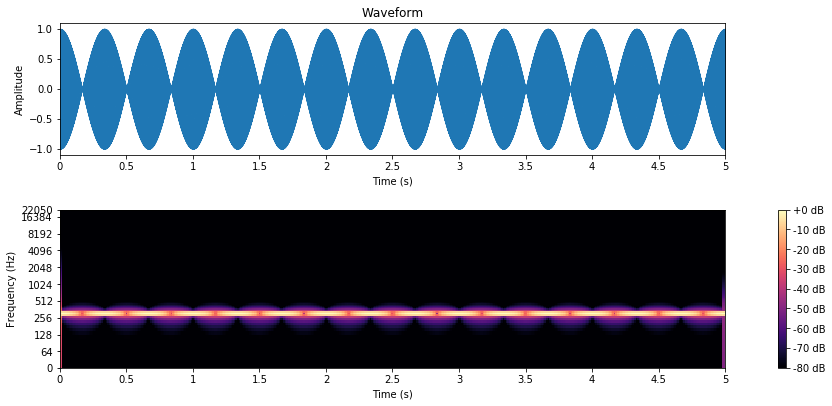
\includegraphics[width=\linewidth]{assets/audio_results/multitoneBeats.png}
        \caption{Spectogram of Ground Truth Multitone Beats Audio}
        \label{fig:gt-multibeat-spec}
    \end{figure}
    
    \begin{figure}[H]
        \centering
        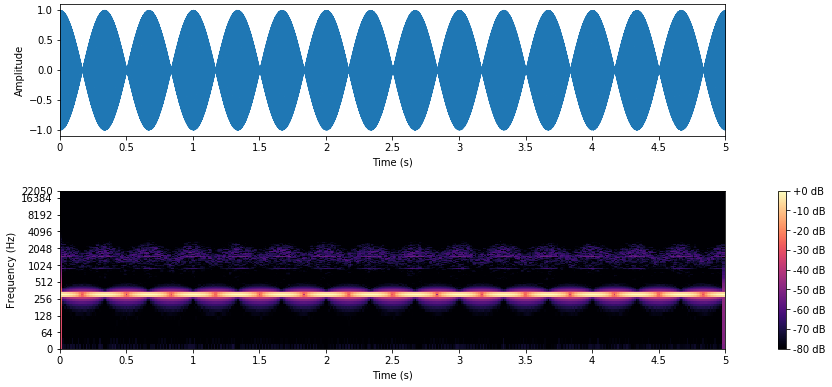
\includegraphics[width=\linewidth]{assets/audio_results/multitoneBeatspred.png}
        \caption{Spectogram of Predicted Multitone Beats Audio}
        \label{fig:pred-multibeat-spec}
    \end{figure}

Across various audio processing tests—including sweeping tone, fluctuating tone, multitone A4E4, and multitone beats—the discrepancies between ground truth and predicted audio files reveal consistent patterns of fidelity loss and signal inaccuracies. The sweeping tone case highlights the most pronounced differences, where the ground truth displays a clean, linear frequency sweep from 200 to 500Hz with well-defined energy bands. In contrast, the predicted audio shows significant degradation with a noisy spectral representation, losing the clear linear progression and displaying additional spectral artifacts that muddy the intended sweep. This indicates substantial challenges in the model's handling of dynamic frequency changes, where precision in representing linear frequency transitions is crucial but not adequately preserved.

In the other cases, similar issues of spectral blurring and noise introduction are evident. The fluctuating 400Hz tone shows a well-maintained singular frequency focus in the ground truth, whereas the predicted audio introduces noise at unrelated frequencies, slightly distorting the clarity of the 400Hz tone. The multitone A4E4 and beats cases both demonstrate a reduction in spectral and waveform clarity in the predicted outputs. For A4E4, the clear separation of tones blurs, and additional noise appears around 3000 Hz, while in the beats case, rhythmic structures are generally retained but with compromised sharpness and added background noise, affecting the waveform’s precision in timing and amplitude.


    \begin{figure}[H]
        \centering
        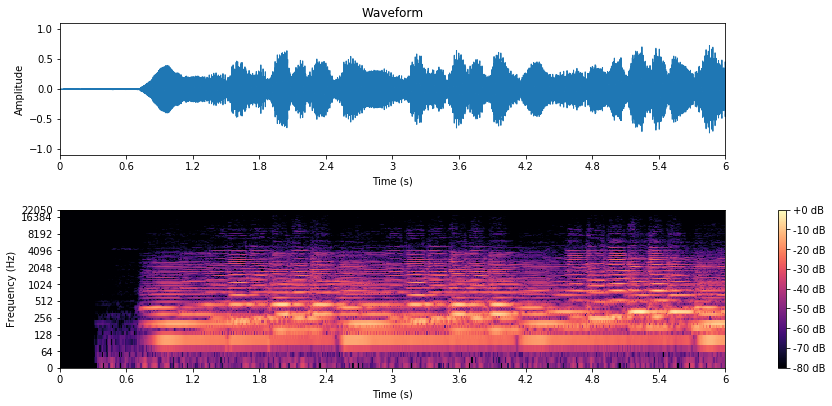
\includegraphics[width=\linewidth]{assets/audio_results/06seconds.png}
        \caption{Spectogram of Ground Truth 6 Seconds Audio}
        \label{fig:gt-6s-spec}
    \end{figure}
    
    \begin{figure}[H]
        \centering
        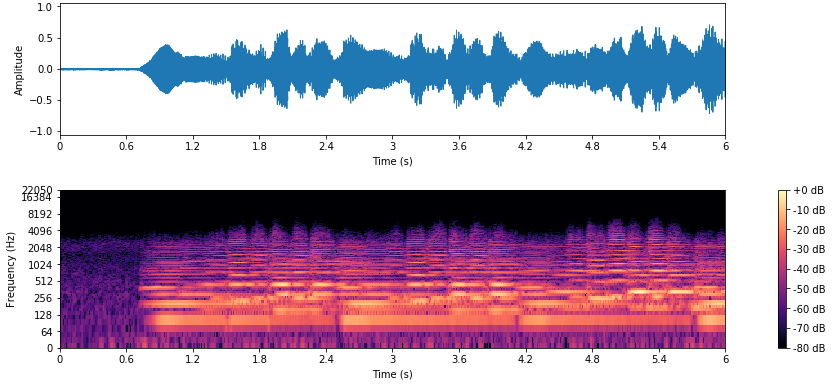
\includegraphics[width=\linewidth]{assets/audio_results/06secondspred.png}
        \caption{Spectogram of Predicted 6 Seconds Audio}
        \label{fig:pred-6s-spec}
    \end{figure}

    \begin{figure}[H]
        \centering
        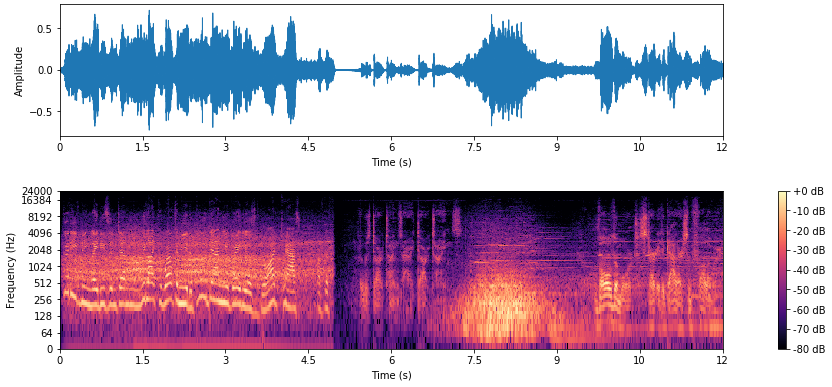
\includegraphics[width=\linewidth]{assets/audio_results/12seconds.png}
        \caption{Spectogram of Ground Truth 12 Seconds Audio}
        \label{fig:gt-12s-spec}
    \end{figure}
    
    \begin{figure}[H]
        \centering
        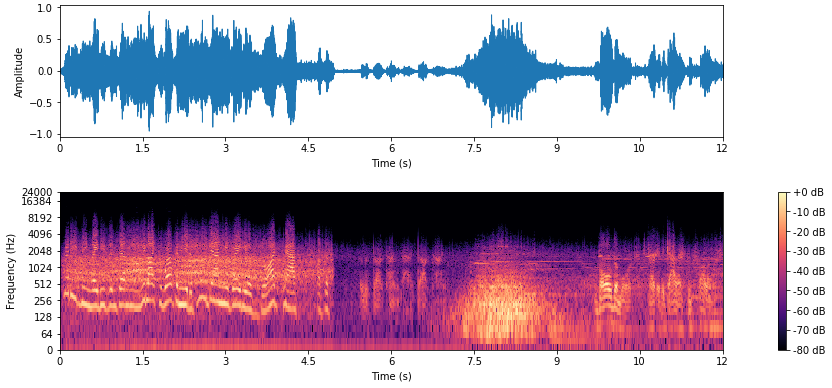
\includegraphics[width=\linewidth]{assets/audio_results/12secondspred.png}
        \caption{Spectogram of Predicted 12 Seconds Audio}
        \label{fig:pred-12s-spec}
    \end{figure}

    \begin{figure}[H]
        \centering
        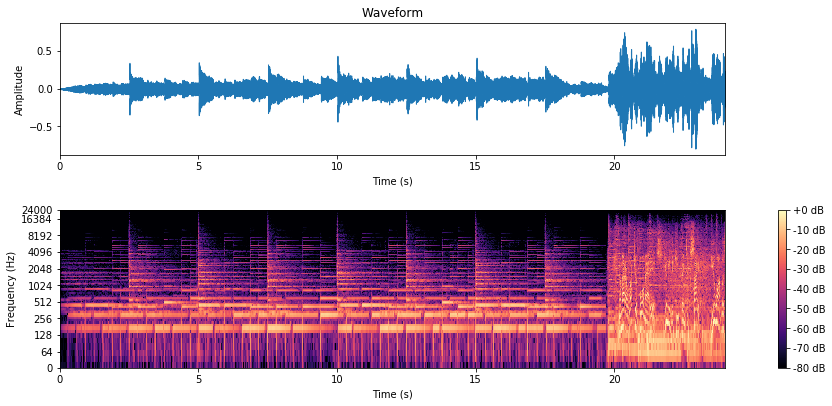
\includegraphics[width=\linewidth]{assets/audio_results/24seconds.png}
        \caption{Spectogram of Ground Truth 24 Seconds Audio}
        \label{fig:gt-24s-spec}
    \end{figure}
    
    \begin{figure}[H]
        \centering
        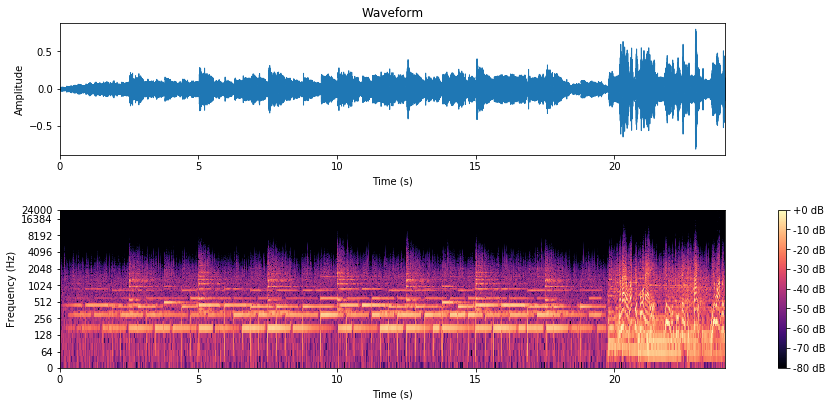
\includegraphics[width=\linewidth]{assets/audio_results/24secondspred.png}
        \caption{Spectogram of Predicted 24 Seconds Audio}
        \label{fig:pred-24s-spec}
    \end{figure}
    
    \begin{figure}[H]
        \centering
        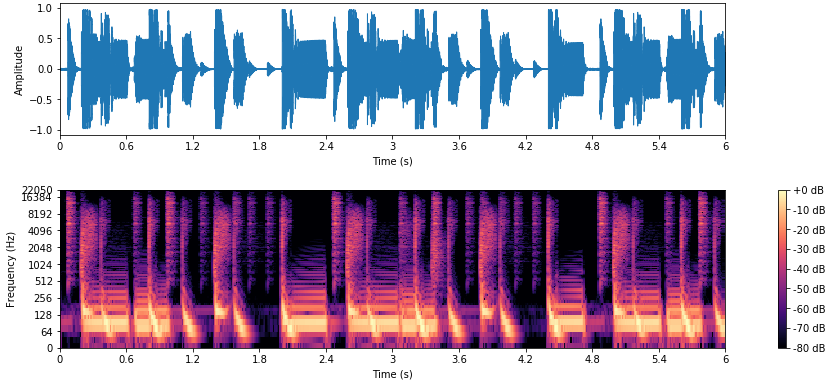
\includegraphics[width=\linewidth]{assets/audio_results/music.png}
        \caption{Spectogram of Ground Truth Music Audio}
        \label{fig:gt-music-spec}
    \end{figure}
    
    \begin{figure}[H]
        \centering
        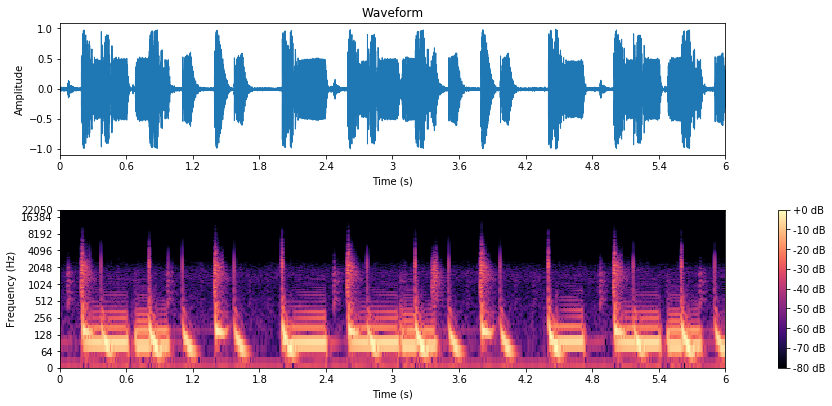
\includegraphics[width=\linewidth]{assets/audio_results/musicpred.png}
        \caption{Spectogram of Predicted Music Audio}
        \label{fig:pred-music-spec}
    \end{figure}

    
    In all four comparisons across different durations of audio—6 seconds, 12 seconds, 24 seconds, and the music segment—the predicted audio consistently displays a reduction in detail and fidelity compared to the ground truth. The waveform of the predicted audio appears to mimic the general shape of the ground truth waveform which suggest the model has captured the overall temporal structure of the audio signal. However upon closer inspection, several differences become apparent. The predicted waveform shows slight discrepancies in amplitude variation compared to the ground truth, indicating that the model has not perfectly replicated the dynamic range of the original audio signal.The waveforms of the predicted audio are generally smoother and more compressed, lacking the dynamic amplitude variations evident in the ground truth, which show sharper peaks and deeper troughs. 
    
    Additionally, the predicted spectrogram exhibits noticeable variations in frequency content; while the general pattern of harmonics is present, some frequency bands appear less defined or slightly shifted compared to the ground truth. The intensity levels in the predicted spectrogram also differ, with certain areas showing reduced or heightened intensity, suggesting variations in loudness or timbre compared to the original. Spectrogram analysis further reveals that the predicted audio tends to have less vibrant colors and reduced frequency activity, particularly in the higher frequency ranges. This muted frequency response suggests a simplification in the audio's complexity and a loss of fine detail, indicating that the prediction models might be averaging or smoothing over nuances present in the original audio signals. The temporal alignment of frequency components in the predicted spectrogram shows minor deviations from the ground truth, indicating that the model may have introduced slight timing errors in reproducing the audio signal.
    \subsubsection{Evaluation Metrics}
    \begin{table}[H]
    \caption{PSNR and LSD values for audio data}
    \centering
    \begin{tabular}{|c|c|c|c|}
        \hline
        \textbf{SN} & \textbf{File Name} & \textbf{PSNR} & \textbf{LSD} \\
        \hline
        1  & puretone100hz & 48.39 & 1.95  \\
        \hline
        2  & puretone500hz & 42.79 & 4.39  \\
        \hline
        3  & puretone1000hz & 22.37 & 7.97  \\
        \hline
        4  & puretone5000hz & 3.01  & 14.24 \\
        \hline
        5  & sweeping\_tone200-500hz & 37.00 & 4.15  \\
        \hline
        6  & fluctuating\_tone400 & 34.79 & 5.92  \\
        \hline
        7  & multitoneA4E4 & 47.93 & 5.19  \\
        \hline
        8  & multitoneBeats & 52.94 & 2.61  \\
        \hline
        9  & 06seconds & 37.11 & 5.82  \\
        \hline
        10 & 12seconds & 31.66 & 10.23 \\
        \hline
        11 & 24seconds & 28.84 & 11.38 \\
        \hline
        12 & music & 23.16 & 15.98 \\
        \hline
    \end{tabular}
    \label{tab:audio_metrics_ordered}
\end{table}

From the above table, we can see that Audio 1 exhibits the highest PSNR value of 48.39 dB, indicating that the predicted audio is very close to the original with minimal distortion. Similarly, Audio 2 and Audio 3 show high PSNR values of 42.79 dB and 22.37 dB, respectively, reflecting strong fidelity in the predictions for these samples. These results suggest that the architecture is effective with simple, low-frequency tones.

Conversely, Audio 4 shows a significantly lower PSNR of 3.01 dB, highlighting a substantial deviation from the original audio. This low PSNR indicates considerable distortion and poor prediction quality for this high-frequency tone. Additionally, Audio 12 has a PSNR of 23.16 dB, which is relatively low compared to other samples, pointing to noticeable discrepancies between the predicted and original signals.

The LSD values provide further insight into spectral distortion. Audio 1 has the lowest LSD value of 1.95, signifying minimal spectral distortion and high prediction quality. On the other hand, Audio 4 has the highest LSD value of 14.24, indicating significant spectral distortion and poorer prediction quality. The LSD values underscore how well the model preserves spectral characteristics, with lower values indicating better performance.

Overall, the variation in PSNR and LSD values among the different audio samples highlights the impact of audio content on prediction performance. While the model achieves high accuracy and minimal distortion for some samples, others, particularly those with complex or high-frequency content, demonstrate poorer quality.


\subsubsection{Histogram of Weights, Biases for Audio 1}


    \begin{figure}[H]
        \centering
        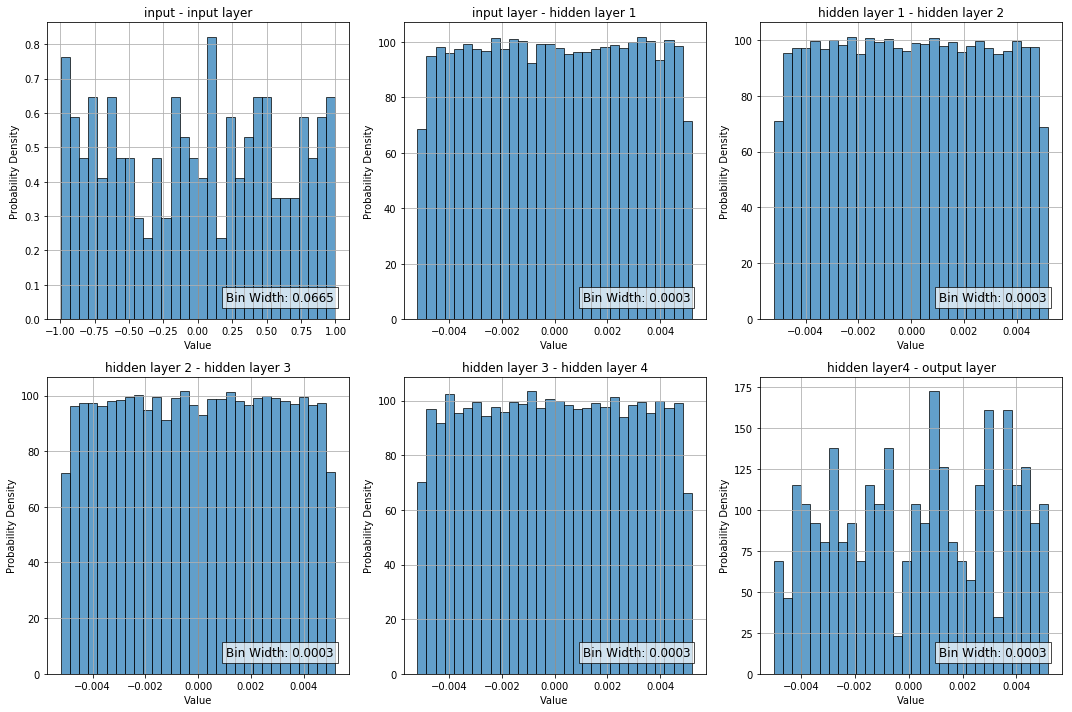
\includegraphics[width=\linewidth]{assets/audio histogram/epoch0Weight.png}
        \caption{Histogram of Weights at Epoch 0}
        \label{fig:audio-weight-0}
    \end{figure}

    \begin{figure}[H]
        \centering
        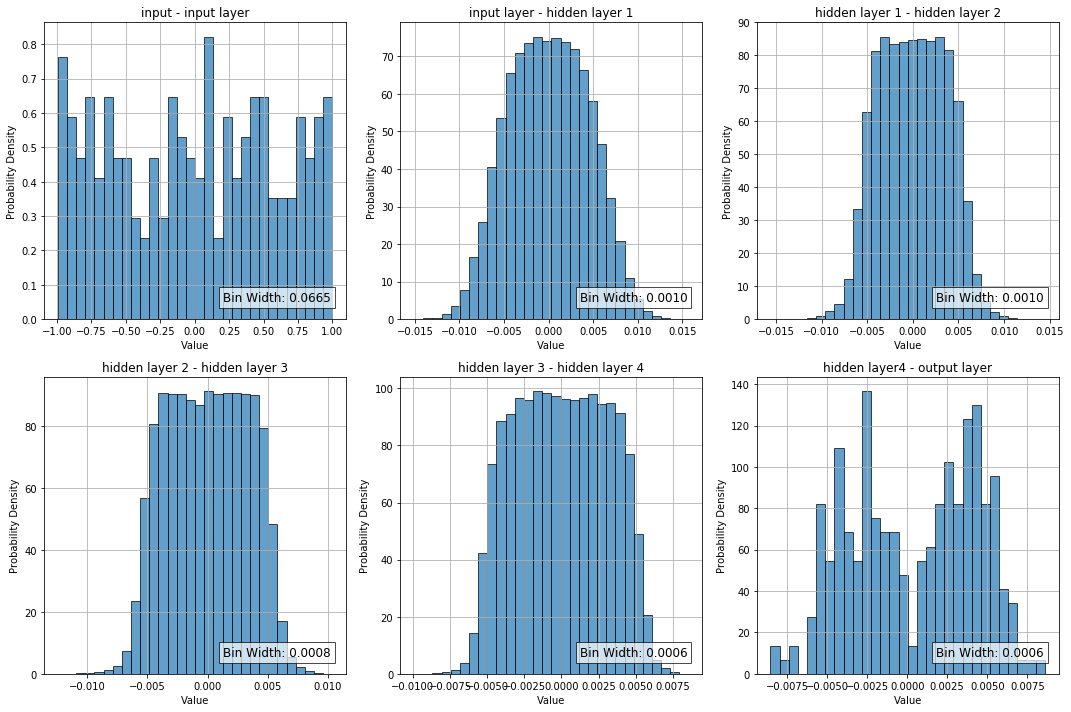
\includegraphics[width=\linewidth]{assets/audio histogram/epoch300Weight.png}
        \caption{Histogram of Weights at Epoch 300}
        \label{fig:audio-weight-300}
    \end{figure}

    \begin{figure}[H]
        \centering
        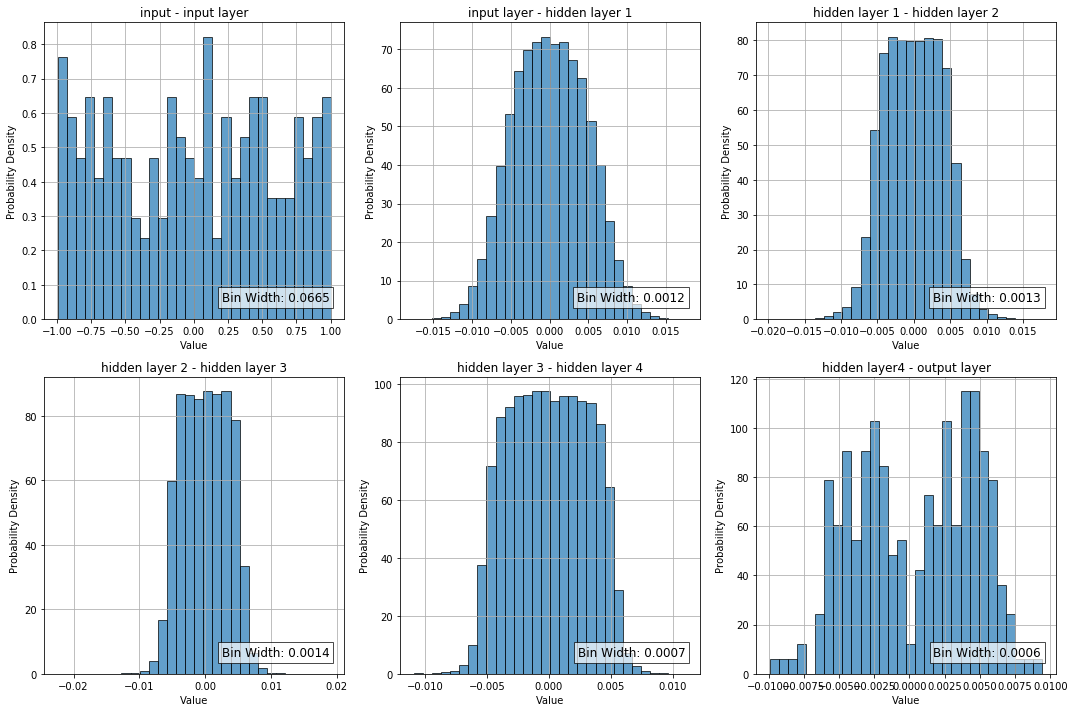
\includegraphics[width=\linewidth]{assets/audio histogram/epoch600Weight.png}
        \caption{Histogram of Weights at Epoch 600}
        \label{fig:audio-weight-600}
    \end{figure}

    \begin{figure}[H]
        \centering
        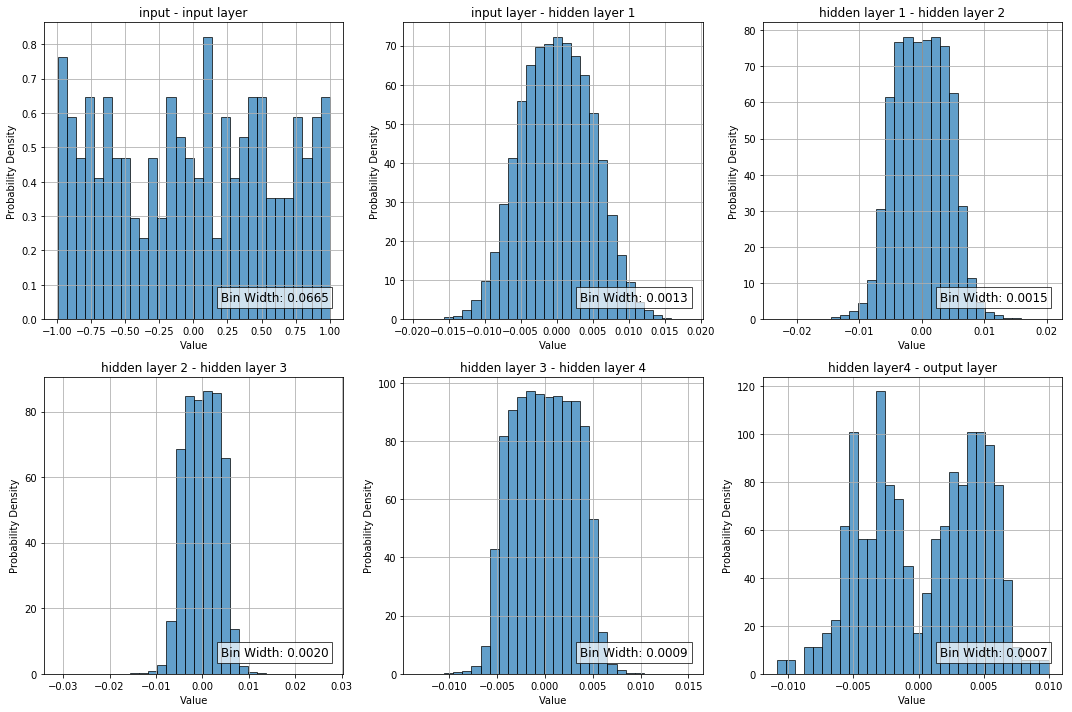
\includegraphics[width=\linewidth]{assets/audio histogram/epoch999Weight.png}
        \caption{Histogram of Weights at Epoch 999}
        \label{fig:audio-weight-999}
    \end{figure}


    \begin{figure}[H]
        \centering
        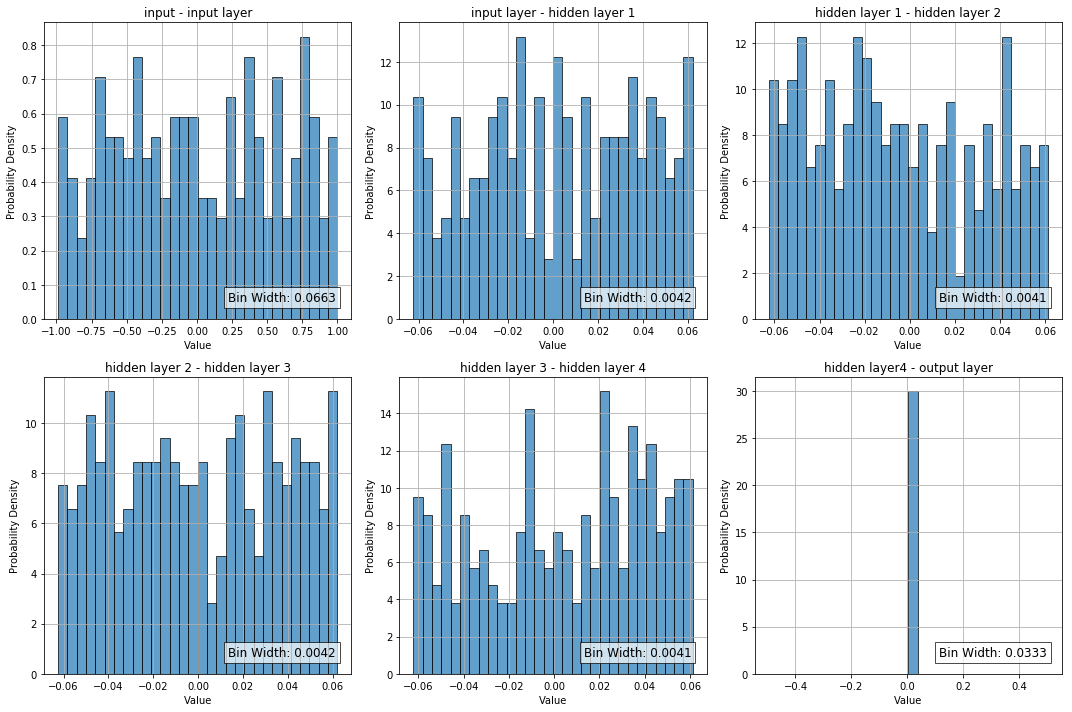
\includegraphics[width=\linewidth]{assets/audio histogram/epoch0Bias.png}
        \caption{Histogram of Bias at Epoch 0}
        \label{fig:audio-bias-0}
    \end{figure}

    \begin{figure}[H]
        \centering
        \includegraphics[width=\linewidth]{assets/audio histogram/epoch300Bias.png}
        \caption{Histogram of Bias at Epoch 300}
        \label{fig:audio-bias-300}
    \end{figure}

    \begin{figure}[H]
        \centering
        \includegraphics[width=\linewidth]{assets/audio histogram/epoch600Bias.png}
        \caption{Histogram of Bias at Epoch 600}
        \label{fig:audio-bias-600}
    \end{figure}

    \begin{figure}[H]
        \centering
        \includegraphics[width=\linewidth]{assets/audio histogram/epoch999Bias.png}
        \caption{Histogram of Bias at Epoch 999}
        \label{fig:audio-bias-999}
    \end{figure}

    \begin{table}[H]
    \centering
    \begin{tabular}{|l|c|c|c|}
    \hline
    \multirow{2}{*}{\textbf{Layer}} & \multicolumn{3}{|c|}{\textbf{KL Divergence (Weights)}} \\
    \cline{2-4}
    & \textbf{Epoch 0 - 300} & \textbf{Epoch 300 - 600} & \textbf{Epoch 600 - 999} \\
    \hline
    input - input layer & 0.000006 & 0.000000 & 0.000000 \\
    input layer - hidden layer 1 & 1.556353 & 0.124401 & 0.090967 \\
    hidden layer 1 - hidden layer 2 & 0.420411 & 0.042276 & 0.035750 \\
    hidden layer 2 - hidden layer 3 & 0.210519 & 0.018601 & 0.013199 \\
    hidden layer 3 - hidden layer 4 & 0.244147 & 0.009357 & 0.006045 \\
    hidden layer 4 - output layer & 0.155492 & 0.000728 & 0.000372 \\
    \hline
    \end{tabular}
    \caption{KL Divergence for Weights}
    \end{table}

    \begin{table}[H]
    \centering
    \begin{tabular}{|l|c|c|c|}
    \hline
    \multirow{2}{*}{\textbf{Layer}} & \multicolumn{3}{|c|}{\textbf{Earth Mover's Distance (Weights)}} \\
    \cline{2-4}
    & \textbf{Epoch 0 - 300} & \textbf{Epoch 300 - 600} & \textbf{Epoch 600 - 999} \\
    \hline
    input - input layer & 0.000192 & 0.000010 & 0.000009 \\
    input layer - hidden layer 1 & 0.001151 & 0.000205 & 0.000113 \\
    hidden layer 1 - hidden layer 2 & 0.000543 & 0.000218 & 0.000159 \\
    hidden layer 2 - hidden layer 3 & 0.000293 & 0.000130 & 0.000093 \\
    hidden layer 3 - hidden layer 4 & 0.000102 & 0.000033 & 0.000026 \\
    hidden layer 4 - output layer & 0.000953 & 0.000258 & 0.000170 \\
    \hline
    \end{tabular}
    \caption{Earth Mover's Distance for Weights}
    \end{table}

    \begin{table}[H]
    \centering
    \begin{tabular}{|l|c|c|c|}
    \hline
    \multirow{2}{*}{\textbf{Layer}} & \multicolumn{3}{|c|}{\textbf{Earth Mover's Distance (Weights)}} \\
    \cline{2-4}
    & \textbf{Epoch 0 - 300} & \textbf{Epoch 300 - 600} & \textbf{Epoch 600 - 999} \\
    \hline
    input - input layer & 0.000192 & 0.000010 & 0.000009 \\
    input layer - hidden layer 1 & 0.001151 & 0.000205 & 0.000113 \\
    hidden layer 1 - hidden layer 2 & 0.000543 & 0.000218 & 0.000159 \\
    hidden layer 2 - hidden layer 3 & 0.000293 & 0.000130 & 0.000093 \\
    hidden layer 3 - hidden layer 4 & 0.000102 & 0.000033 & 0.000026 \\
    hidden layer 4 - output layer & 0.000953 & 0.000258 & 0.000170 \\
    \hline
    \end{tabular}
    \caption{Earth Mover's Distance for Weights}
    \end{table}


    \begin{table}[H]
    \centering
    \begin{tabular}{|l|c|c|c|}
    \hline
    \multirow{2}{*}{\textbf{Layer}} & \multicolumn{3}{|c|}{\textbf{KL Divergence (Biases)}} \\
    \cline{2-4}
    & \textbf{Epoch 0 - 300} & \textbf{Epoch 300 - 600} & \textbf{Epoch 600 - 999} \\
    \hline
    input - input layer & 0.000015 & 0.000001 & 0.000001 \\
    input layer - hidden layer 1 & 0.001897 & 0.000149 & 0.000110 \\
    hidden layer 1 - hidden layer 2 & 0.000474 & 0.000036 & 0.000019 \\
    hidden layer 2 - hidden layer 3 & 0.001169 & 0.000007 & 0.000004 \\
    hidden layer 3 - hidden layer 4 & 0.000371 & 0.000003 & 0.000004 \\
    hidden layer 4 - output layer & 0.000000 & 0.000000 & 0.000000 \\
    \hline
    \end{tabular}
    \caption{KL Divergence for Biases}
    \end{table}

    
    The KL Divergence (Kullback-Leibler Divergence) for weights shows a decreasing trend across the epochs for each layer. Initially, the KL Divergence values are highest in the earlier epochs (0-300) and reduce significantly as the training progresses (300-600 and 600-999 epochs). For instance, the KL Divergence between the input layer and hidden layer 1 starts at 1.556353 in the initial epoch range, dropping to 0.124401 and further to 0.090967 in the later epochs. This consistent reduction indicates that the model's weights are becoming more stable and optimized as training progresses, suggesting a successful learning process and effective weight adjustment towards minimizing the divergence between the distributions.

    The Earth Mover's Distance (EMD) for weights also exhibits a similar downward trend, reflecting the efficiency of the training process. For instance, the EMD between the input layer and hidden layer 1 starts at 0.001151 in the initial epoch range and decreases to 0.000205 and 0.000113 in the subsequent epochs. This reduction in EMD indicates that the distribution of weights between layers is converging and becoming more consistent over time. The trend is consistent across other layers as well, with the initial high values indicating more significant adjustments in the early training phases and lower values in later epochs demonstrating fine-tuning and stabilization of the weights. This overall decrease in both KL Divergence and EMD supports the model's effective training and improved representation learning over time.





\subsubsection{PDF and CDF of Activations for Audio 1}

    \begin{figure}[H]
        \centering
        \includegraphics[width=\linewidth]{assets/audio histogram/epoch0activations.png}
        \caption{PDF and CDF of Activations at Epoch 0}
        \label{fig:audio-activation-0}
    \end{figure}

    \begin{figure}[H]
        \centering
        \includegraphics[width=\linewidth]{assets/audio histogram/epoch300activations.png}
        \caption{PDF and CDF of Activations at Epoch 300}
        \label{fig:audio-activation-300}
    \end{figure}

    \begin{figure}[H]
        \centering
        \includegraphics[width=\linewidth]{assets/audio histogram/epoch600activations.png}
        \caption{PDF and CDF of Activations at Epoch 600}
        \label{fig:audio-activation-600}
    \end{figure}

        \begin{figure}[H]
        \centering
        \includegraphics[width=\linewidth]{assets/audio histogram/epoch999activations.png}
        \caption{PDF and CDF of Activations at Epoch 999}
        \label{fig:audio-activation-999}
    \end{figure}

    The activation plots in this set provide a comprehensive view of how activations are distributed across different layers of the network, both before and after applying sine activation functions. Initially, the input values are uniformly distributed, as depicted by the even distribution in the histogram and the linear cumulative distribution function (CDF).For the input layer with linear activation, the probability density function (PDF) becomes almost normally distributed due to the effect of weights initialization. This normal-like distribution is evident from the bell-shaped histogram and the S-shaped curve in the CDF. However, after applying the sine activation, the PDF transitions towards an arcsine distribution, shown by the histogram peaks at the extremes and the distinct shape of the CDF.

    Moving on to the hidden layers, a similar trend is observed. The first hidden layer with linear activation has a near-normal distribution, as shown by the central peak in the histogram and the corresponding CDF. When sine activation is applied, the distribution changes to resemble an arcsine distribution, with peaks at the boundaries in the histogram and the characteristic shape in the CDF.The second hidden layer also follows this pattern. With linear activation, the distribution remains near-normal, and the sine activation shifts it towards an arcsine distribution. This is consistently seen in the histograms and CDFs for both activations.In the third hidden layer, the linear activation maintains a near-normal distribution, while the sine activation once again transforms the distribution to an arcsine form. The fourth hidden layer exhibits the same behavior, with a near-normal distribution under linear activation and an arcsine distribution with sine activation.

    Finally, the output layer shows a close-to-normal distribution before any non-linear activation is applied, as indicated by the bell-shaped histogram and the normal-like CDF. Overall, these plots clearly demonstrate the transition from uniformly distributed input values through near-normal distributions with linear activations to arcsine-like distributions with sine activations, highlighting the significant impact of the sine function on the activation values throughout the network.



    \subsubsection{Loss Curves}
    \begin{figure}[H]
        \centering
        \includegraphics[width=\linewidth]{assets/audio_loss_curves/puretone100.png}
        \caption{Training Loss curve of Audio 1}
        \label{fig:loss-curve-1}
    \end{figure}
    \begin{figure}[H]
        \centering
        \includegraphics[width=\linewidth]{assets/audio_loss_curves/puretone500.png}
        \caption{Training Loss curve of Audio 2}
        \label{fig:loss-curve-2}
    \end{figure}
    \begin{figure}[H]
        \centering
        \includegraphics[width=\linewidth]{assets/audio_loss_curves/puretone1000.png}
        \caption{Training Loss curve of Audio 3}
        \label{fig:loss-curve-3}
    \end{figure}
    \begin{figure}[H]
        \centering
        \includegraphics[width=\linewidth]{assets/audio_loss_curves/puretone5000.png}
        \caption{Training Loss curve of Audio 4}
        \label{fig:loss-curve-4}
    \end{figure}
    \begin{figure}[H]
        \centering
        \includegraphics[width=\linewidth]{assets/audio_loss_curves/sweepingtone200_500.png}
        \caption{Training Loss curve of Audio 5}
        \label{fig:loss-curve-5}
    \end{figure}
    \begin{figure}[H]
        \centering
        \includegraphics[width=\linewidth]{assets/audio_loss_curves/fluctuating_tone400.png}
        \caption{Training Loss curve of Audio 6}
        \label{fig:loss-curve-6}
    \end{figure}
    \begin{figure}[H]
        \centering
        \includegraphics[width=\linewidth]{assets/audio_loss_curves/multitone_a4e4.png}
        \caption{Training Loss curve of Audio 7}
        \label{fig:loss-curve-7}
    \end{figure}
    \begin{figure}[H]
        \centering
        \includegraphics[width=\linewidth]{assets/audio_loss_curves/multitone_beats.png}
        \caption{Training Loss curve of Audio 8}
        \label{fig:loss-curve-8}
    \end{figure}
    \begin{figure}[H]
        \centering
        \includegraphics[width=\linewidth]{assets/audio_loss_curves/06seconds.png}
        \caption{Training Loss curve of Audio 9}
        \label{fig:loss-curve-9}
    \end{figure}
    \begin{figure}[H]
        \centering
        \includegraphics[width=\linewidth]{assets/audio_loss_curves/12seconds.png}
        \caption{Training Loss curve of Audio 10}
        \label{fig:loss-curve-10}
    \end{figure}
    \begin{figure}[H]
        \centering
        \includegraphics[width=\linewidth]{assets/audio_loss_curves/24seconds.png}
        \caption{Training Loss curve of Audio 11}
        \label{fig:loss-curve-11}
    \end{figure}
    \begin{figure}[H]
        \centering
        \includegraphics[width=\linewidth]{assets/audio_loss_curves/music_with_instrument.png}
        \caption{Training Loss curve of Audio 12}
        \label{fig:loss-curve-12}
    \end{figure}


    \subsection{Video Dataset}
    Below are the grouth truth images and the predicted images of first video dataset.

    \begin{figure}[H]
    \centering
    \begin{minipage}{0.45\textwidth}
        \centering
        \includegraphics[width=\linewidth]{assets/video_results/im1.png}
        \caption{Ground Truth Frame 1}
        \label{fig:gt-frame-1}
    \end{minipage}\hfill
    \begin{minipage}{0.45\textwidth}
        \centering
        \includegraphics[width=\linewidth]{assets/video_results/pred0.png}
        \caption{Predicted Frame 1}
        \label{fig:pred-frame-1}
    \end{minipage}
\end{figure}
    \begin{figure}[H]
    \centering
    \begin{minipage}{0.45\textwidth}
        \centering
        \includegraphics[width=\linewidth]{assets/video_results/im2.png}
        \caption{Ground Truth Frame 2}
        \label{fig:gt-frame-2}
    \end{minipage}\hfill
    \begin{minipage}{0.45\textwidth}
        \centering
        \includegraphics[width=\linewidth]{assets/video_results/pred1.png}
        \caption{Predicted Frame 2}
        \label{fig:pred-frame-2}
    \end{minipage}
\end{figure}
    \begin{figure}[H]
    \centering
    \begin{minipage}{0.45\textwidth}
        \centering
        \includegraphics[width=\linewidth]{assets/video_results/im3.png}
        \caption{Ground Truth Frame 3}
        \label{fig:gt-frame-3}
    \end{minipage}\hfill
    \begin{minipage}{0.45\textwidth}
        \centering
        \includegraphics[width=\linewidth]{assets/video_results/pred2.png}
        \caption{Predicted Frame 3}
        \label{fig:pred-frame-3}
    \end{minipage}
\end{figure}

    \begin{figure}[H]
    \centering
    \begin{minipage}{0.45\textwidth}
        \centering
        \includegraphics[width=\linewidth]{assets/video_results/im4.png}
        \caption{Ground Truth Frame 4}
        \label{fig:gt-frame-4}
    \end{minipage}\hfill
    \begin{minipage}{0.45\textwidth}
        \centering
        \includegraphics[width=\linewidth]{assets/video_results/pred3.png}
        \caption{Predicted Frame 4}
        \label{fig:pred-frame-4}
    \end{minipage}
\end{figure}
\begin{figure}[H]
    \centering
    \begin{minipage}{0.45\textwidth}
        \centering
        \includegraphics[width=\linewidth]{assets/video_results/im5.png}
        \caption{Ground Truth Frame 5}
        \label{fig:gt-frame-5}
    \end{minipage}\hfill
    \begin{minipage}{0.45\textwidth}
        \centering
        \includegraphics[width=\linewidth]{assets/video_results/pred4.png}
        \caption{Predicted Frame 5}
        \label{fig:pred-frame-5}
    \end{minipage}
\end{figure}

\subsubsection{Evaluation Metrics}
\begin{table}[H]
    \caption{PSNR, SSIM, and LPIPS values for video data}
    \centering
    \begin{tabular}{|c|c|c|c|c|}
        \hline
        \textbf{SN} & \textbf{Video} & \textbf{PSNR} & \textbf{SSIM} & \textbf{LPIPS} \\
        \hline
        1 & very\_very\_short\_video & 29.0736 & 0.8749 & 0.0699 \\ 
        \hline
        2 & very\_short\_video & 28.8302 & 0.8982 & 0.0869 \\ 
        \hline
        3 & short\_video & 27.4749 & 0.8579 & 0.1820 \\ 
        \hline
        4 & medium\_video & 23.4656 & 0.8875 & 0.1927 \\ 
        \hline
        5 & long\_video & 24.4722 & 0.8695 & 0.2386 \\ 
        \bottomrule
    \end{tabular}
    \label{tab:video_metrics}
\end{table}
In our results, Video 1 achieves the highest PSNR value of 29.0736, suggesting it retains the highest level of detail with minimal distortion. Conversely, Video 4 has the lowest PSNR value of 23.4656, indicating a higher level of noise or distortion introduced during compression.

Video 2 has the highest SSIM score of 0.8982, indicating that its structural content closely resembles the original. In contrast, Video 3 has the lowest SSIM score of 0.8579, suggesting a slight reduction in structural similarity compared to the other videos.

 Video 1 stands out with the lowest LPIPS value of 0.0699, reflecting the highest perceptual fidelity among the videos analyzed. On the other hand, Video 5 shows the highest LPIPS value of 0.2386, indicating more noticeable perceptual differences from the original.

Overall, the results indicate that shorter videos tend to maintain higher visual quality after compression, as evidenced by their higher PSNR and SSIM values and lower LPIPS scores. This trend suggests that it performs optimally on videos with shorter durations or simpler content, where it can better preserve the visual and structural integrity of the video. The varying values across different metrics underscore the trade-offs involved in video compression, with longer videos exhibiting more noticeable degradation.

In conclusion, while the evaluation metrics demonstrate the architecture's strengths in preserving video quality in shorter videos, there is room for optimization to achieve consistent performance across all video types. Improving the architecture to handle longer or more complex videos more effectively could be a focus for future work, ensuring high perceptual quality and structural similarity across various content types.




\subsubsection{Histogram of Weights and Biases for Video 3}


    \begin{figure}[H]
        \centering
        \includegraphics[width=\linewidth]{assets/video histogram/epoch0Weight.png}
        \caption{Histogram of Weights at Epoch 0}
        \label{fig:video-weight-0}
    \end{figure}

    \begin{figure}[H]
        \centering
        \includegraphics[width=\linewidth]{assets/video histogram/epoch700Weight.png}
        \caption{Histogram of Weights at Epoch 700}
        \label{fig:video-weight-700}
    \end{figure}

    \begin{figure}[H]
        \centering
        \includegraphics[width=\linewidth]{assets/video histogram/epoch1500Weight.png}
        \caption{Histogram of Weights at Epoch 1500}
        \label{fig:video-weight-1500}
    \end{figure}

    \begin{figure}[H]
        \centering
        \includegraphics[width=\linewidth]{assets/video histogram/epoch1999Weight.png}
        \caption{Histogram of Weights at Epoch 1999}
        \label{fig:video-weight-1999}
    \end{figure}


    \begin{figure}[H]
        \centering
        \includegraphics[width=\linewidth]{assets/video histogram/epoch0Bias.png}
        \caption{Histogram of Bias at Epoch 0}
        \label{fig:video-bias-0}
    \end{figure}

    \begin{figure}[H]
        \centering
        \includegraphics[width=\linewidth]{assets/video histogram/epoch700Bias.png}
        \caption{Histogram of Bias at Epoch 700}
        \label{fig:video-bias-700}
    \end{figure}

    \begin{figure}[H]
        \centering
        \includegraphics[width=\linewidth]{assets/video histogram/epoch1500Bias.png}
        \caption{Histogram of Bias at Epoch 1500}
        \label{fig:video-bias-1500}
    \end{figure}

    \begin{figure}[H]
        \centering
        \includegraphics[width=\linewidth]{assets/video histogram/epoch1999Bias.png}
        \caption{Histogram of Bias at Epoch 1999}
        \label{fig:video-bias-1999}
    \end{figure}

    \begin{table}[H]
    \centering
    \begin{tabular}{|l|c|c|c|}
    \hline
    \multirow{2}{*}{\textbf{Layer}} & \multicolumn{3}{|c|}{\textbf{KL Divergence (Weights)}} \\
    \cline{2-4}
    & \textbf{Epoch 0 - 700} & \textbf{Epoch 700 - 1500} & \textbf{Epoch 1500 - 1999} \\
    \hline
    input - input layer & 0.000161 & 0.000049 & 0.000046 \\
    input layer - hidden layer 1 & 1.362321 & 0.179672 & 0.122370 \\
    hidden layer 1 - hidden layer 2 & 1.138587 & 0.414731 & 0.281766 \\
    hidden layer 2 - hidden layer 3 & 17.374886 & 0.267125 & 0.224011 \\
    hidden layer 3 - hidden layer 4 & 0.608277 & 0.323486 & 18.722935 \\
    hidden layer 4 - output layer & 1.306046 & 0.046368 & 0.021945 \\
    \hline
    \end{tabular}
    \caption{KL Divergence for Weights}
    \end{table}

    \begin{table}[H]
    \centering
    \begin{tabular}{|l|c|c|c|}
    \hline
    \multirow{2}{*}{\textbf{Layer}} & \multicolumn{3}{|c|}{\textbf{Earth Mover's Distance (Weights)}} \\
    \cline{2-4}
    & \textbf{Epoch 0 - 700} & \textbf{Epoch 700 - 1500} & \textbf{Epoch 1500 - 1999} \\
    \hline
    input - input layer & 0.000657 & 0.000495 & 0.000316 \\
    input layer - hidden layer 1 & 0.000335 & 0.000102 & 0.000054 \\
    hidden layer 1 - hidden layer 2 & 0.000299 & 0.000112 & 0.000044 \\
    hidden layer 2 - hidden layer 3 & 0.000152 & 0.000057 & 0.000025 \\
    hidden layer 3 - hidden layer 4 & 0.000090 & 0.000051 & 0.000028 \\
    hidden layer 4 - output layer & 0.000757 & 0.000093 & 0.000045 \\
    \hline
    \end{tabular}
    \caption{Earth Mover's Distance for Weights}
    \end{table}

    \begin{table}[H]
    \centering
    \begin{tabular}{|l|c|c|c|}
    \hline
    \multirow{2}{*}{\textbf{Layer}} & \multicolumn{3}{|c|}{\textbf{KL Divergence (Biases)}} \\
    \cline{2-4}
    & \textbf{Epoch 0 - 700} & \textbf{Epoch 700 - 1500} & \textbf{Epoch 1500 - 1999} \\
    \hline
    input - input layer & 0.000044 & 0.000037 & 0.000005 \\
    input layer - hidden layer 1 & 0.004088 & 0.000360 & 0.000422 \\
    hidden layer 1 - hidden layer 2 & 0.016827 & 0.013568 & 0.003450 \\
    hidden layer 2 - hidden layer 3 & 0.036906 & 0.001071 & 0.002715 \\
    hidden layer 3 - hidden layer 4 & 0.003555 & 0.000064 & 0.000076 \\
    hidden layer 4 - output layer & 0.000000 & 0.000000 & 0.000000 \\
    \hline
    \end{tabular}
    \caption{KL Divergence for Biases}
    \end{table}
    
    \begin{table}[H]
    \centering
    \begin{tabular}{|l|c|c|c|}
    \hline
    \multirow{2}{*}{\textbf{Layer}} & \multicolumn{3}{|c|}{\textbf{Earth Mover's Distance (Biases)}} \\
    \cline{2-4}
    & \textbf{Epoch 0 - 700} & \textbf{Epoch 700 - 1500} & \textbf{Epoch 1500 - 1999} \\
    \hline
    input - input layer & 0.000632 & 0.000379 & 0.000288 \\
    input layer - hidden layer 1 & 0.000218 & 0.000088 & 0.000064 \\
    hidden layer 1 - hidden layer 2 & 0.000211 & 0.000177 & 0.000145 \\
    hidden layer 2 - hidden layer 3 & 0.000150 & 0.000081 & 0.000081 \\
    hidden layer 3 - hidden layer 4 & 0.000142 & 0.000064 & 0.000059 \\
    hidden layer 4 - output layer & 0.001341 & 0.000164 & 0.000194 \\
    \hline
    \end{tabular}
    \caption{Earth Mover's Distance for Biases}
    \end{table}


    The KL Divergence (Kullback-Leibler Divergence) for weights shows a clear pattern of decreasing values across epochs, indicating improved alignment between the true distribution and the learned distribution as training progresses. For example, the divergence between hidden layer 2 and hidden layer 3 starts at a high 17.374886 in Epochs 0-700, but drops significantly to 0.267125 and 0.224011 in the subsequent epochs. This reduction signifies the model's convergence and stabilization over time, although there is an unusual spike to 18.722935 in hidden layer 3 to hidden layer 4 during Epochs 1500-1999, suggesting a possible overfitting or complex learning phase. Overall, the decreasing KL Divergence values demonstrate the model's effective learning and adaptation.

    Similarly, the Earth Mover's Distance (EMD) for weights consistently declines throughout the training process, reinforcing the observation of effective learning and stabilization. Initial high EMD values, such as 0.000657 for the input layer in Epochs 0-700, significantly decrease by Epochs 1500-1999, indicating minimal distribution shifts and more stable weight distributions. For instance, the EMD between hidden layer 2 and hidden layer 3 drops from 0.000152 to 0.000025, highlighting the model's convergence towards an optimal solution. This consistent reduction in both KL Divergence and EMD values signifies that the model weights and biases are fine-tuned over time, leading to improved stability and performance of the neural network.


\subsubsection{PDF and CDF of Activations for Video 3}


    \begin{figure}[H]
        \centering
        \includegraphics[width=\linewidth]{assets/video histogram/epoch0activations.png}
        \caption{PDF and CDF of Activations at Epoch 0}
        \label{fig:video-activation-0}
    \end{figure}

    \begin{figure}[H]
        \centering
        \includegraphics[width=\linewidth]{assets/video histogram/epoch700activations.png}
        \caption{PDF and CDF of Activations at Epoch 700}
        \label{fig:video-activation-700}
    \end{figure}

    \begin{figure}[H]
        \centering
        \includegraphics[width=\linewidth]{assets/video histogram/epoch1500activations.png}
        \caption{PDF and CDF of Activations at Epoch 1500}
        \label{fig:video-activation-1500}
    \end{figure}

        \begin{figure}[H]
        \centering
        \includegraphics[width=\linewidth]{assets/video histogram/epoch1999activations.png}
        \caption{PDF and CDF of Activations at Epoch 1999}
        \label{fig:video-activation-1999}
    \end{figure}


    The activation plots illustrate the distribution of activation values for each layer in the network, highlighting both linear and sine activations. Initially, the input values are uniformly distributed, as shown by the even spread in the histogram and the straight-line cumulative distribution function (CDF). Before applying sine activation, the probability density function (PDF) of the input layer, as well as subsequent hidden layers with linear activation, is almost normally distributed. This near-normal distribution is due to the effect of weights initialization, resulting in bell-shaped histograms and S-shaped CDFs indicative of normal distributions.

    When sine activation is applied, the PDFs of the layers transform significantly. The histograms reveal peaks at the boundaries and fewer values in the center, resembling an arcsine distribution. This characteristic shift is evident in the distinctive shape of the CDFs for sine-activated layers. Each hidden layer follows this pattern, where linear activation maintains a near-normal distribution, and sine activation alters it to approximate an arcsine distribution. The output layer also exhibits a close-to-normal distribution, shown by the bell-shaped histogram and the corresponding CDF. 

    \pagebreak


\section{\MakeUppercase{Appendices}}
    \subsection*{Appendix A: Project Schedule}
    \addcontentsline{toc}{subsection}{Appendix A: Project Schedule}
    \begin{figure}[H]
        \centering
        \includegraphics[angle=90, origin=c, height=0.65\textheight]{assets/Gantt.png}
        \caption{Gantt Chart}
        \label{fig:gantt}
    \end{figure}
    
\pagebreak

\subsection*{Appendix B: Forward and Backward Propagation}
\label{app:forward-backward-eqn}
\addcontentsline{toc}{subsection}{Appendix B: Forward and Backward Propagation}

\subsubsection*{\MakeUppercase{Forward Propagation}}
\textbf{Step 1: Input to Input Layer}
\begin{itemize}
  \item Input Vector $\mathbf{x}$: Dimension $2 \times 1$
  \item Weight Matrix $\mathbf{W}^{(in)}$: Dimension $2 \times 2$
  \item Bias Vector $\mathbf{b}^{(in)}$: Dimension $2 \times 1$
  \item Calculation:
  \[
  \mathbf{z}^{(in)} = \mathbf{W}^{(in)} \mathbf{x} + \mathbf{b}^{(in)}
  \]
  \[
  \mathbf{a}^{(in)} = \mathbf{z}^{(in)}
  \]
  Where $\mathbf{z}^{(in)}$ and $\mathbf{a}^{(in)}$ both have dimensions $2 \times 1$.
\end{itemize}


\textbf{Step 2: Input Layer to Hidden Layer 1}
\begin{itemize}
  \item Input Vector $\mathbf{x}$: Dimension $2 \times 1$
  \item Weight Matrix $\mathbf{W}^{(1)}$: Dimension $25 \times 2$
  \item Bias Vector $\mathbf{b}^{(1)}$: Dimension $25 \times 1$
  \item Calculation:
  \[
  \mathbf{z}^{(1)} = \mathbf{W}^{(1)} \mathbf{x} + \mathbf{b}^{(1)}
  \]
  \[
  \mathbf{a}^{(1)} = \sin(\mathbf{z}^{(1)})
  \]
  Where $\mathbf{z}^{(1)}$ and $\mathbf{a}^{(1)}$ both have dimensions $25 \times 1$.
\end{itemize}

\textbf{Step 3: Hidden Layer 1 to Hidden Layer 2}
\begin{itemize}
  \item Weight Matrix $\mathbf{W}^{(2)}$: Dimension $25 \times 25$
  \item Bias Vector $\mathbf{b}^{(2)}$: Dimension $25 \times 1$
  \item Calculation:
  \[
  \mathbf{z}^{(2)} = \mathbf{W}^{(2)} \mathbf{a}^{(1)} + \mathbf{b}^{(2)}
  \]
  \[
  \mathbf{a}^{(2)} = \sin(\mathbf{z}^{(2)})
  \]
  Both $\mathbf{z}^{(2)}$ and $\mathbf{a}^{(2)}$ are $25 \times 1$.
\end{itemize}

\textbf{Step 4: Hidden Layer 2 to Output Layer}
\begin{itemize}
  \item Weight Matrix $\mathbf{W}^{(3)}$: Dimension $3 \times 25$
  \item Bias Vector $\mathbf{b}^{(3)}$: Dimension $3 \times 1$
  \item Calculation:
  \[
  \mathbf{z}^{(3)} = \mathbf{W}^{(3)} \mathbf{a}^{(2)} + \mathbf{b}^{(3)}
  \]
  \[
  \mathbf{a}^{(3)} = \sin(\mathbf{z}^{(3)})
  \]
  Where $\mathbf{z}^{(3)}$ and $\mathbf{a}^{(3)}$ both have dimensions $3 \times 1$.
\end{itemize}


\subsubsection*{\MakeUppercase{Backpropagation}}

\textbf{Step 1: Output Layer to Hidden Layer 2}
\begin{enumerate}[label=\textbf{\roman*.}]
  \item \textbf{Gradient of Loss with respect to output activations} $(\mathbf{a}^{(3)})$:
  
  Given the Mean Squared Error (MSE) loss function:
  \[
  \text{Loss} = \frac{1}{2} \sum_{i=1}^{3} (y_i - a^{(3)}_i)^2
  \]
  Differentiate Loss w.r.t. $\mathbf{a}^{(3)}$:
  \[
  \frac{\partial \text{Loss}}{\partial a^{(3)}_i} = a^{(3)}_i - y_i
  \]
  This will result in a vector $\mathbf{a}^{(3)} - \mathbf{y}$.

  \item \textbf{Gradient with respect to} $\mathbf{z}^{(3)}$ (using chain rule and recognizing $\mathbf{a}^{(3)} = \sin(\mathbf{z}^{(3)})$):
  \[
  \frac{\partial \text{Loss}}{\partial \mathbf{z}^{(3)}} = \frac{\partial \text{Loss}}{\partial \mathbf{a}^{(3)}} \cdot \frac{\partial \mathbf{a}^{(3)}}{\partial \mathbf{z}^{(3)}}
  \]
  Since $\frac{\partial a^{(3)}_i}{\partial z^{(3)}_i} = \cos(z^{(3)}_i)$, the gradient becomes:
  \[
  \frac{\partial \text{Loss}}{\partial \mathbf{z}^{(3)}} = (\mathbf{a}^{(3)} - \mathbf{y}) \cdot \cos(\mathbf{z}^{(3)})
  \]

  \item \textbf{Gradient with respect to weights} $\mathbf{W}^{(3)}$ \textbf{and biases} $\mathbf{b}^{(3)}$:
  
  \[
  \frac{\partial \text{Loss}}{\partial \mathbf{W}^{(3)}} = \frac{\partial \text{Loss}}{\partial \mathbf{z}^{(3)}} \cdot \frac{\partial \mathbf{z}^{(3)}}{\partial \mathbf{W}^{(3)}}
  \]
  
  \[
  \frac{\partial \text{Loss}}{\partial \mathbf{W}^{(3)}} = \frac{\partial \text{Loss}}{\partial \mathbf{z}^{(3)}} \mathbf{a}^{(2)T}
  \]
  
  \[
  \frac{\partial \text{Loss}}{\partial \mathbf{W}^{(3)}} = \left((\mathbf{a}^{(3)} - \mathbf{y}) \cdot \cos(\mathbf{z}^{(3)})\right) \mathbf{a}^{(2)T}
  \]


  \[
  \frac{\partial \text{Loss}}{\partial \mathbf{b}^{(3)}} = \frac{\partial \text{Loss}}{\partial \mathbf{z}^{(3)}} \cdot \frac{\partial \mathbf{z}^{(3)}}{\partial \mathbf{b}^{(3)}}
  \]

  \[
  \frac{\partial \text{Loss}}{\partial \mathbf{b}^{(3)}} = \frac{\partial \text{Loss}}{\partial \mathbf{z}^{(3)}}
  \]

  \[
  \frac{\partial \text{Loss}}{\partial \mathbf{b}^{(3)}} = (\mathbf{a}^{(3)} - \mathbf{y}) \cdot \cos(\mathbf{z}^{(3)})
  \]
  
\end{enumerate}

\textbf{Step 2: Hidden Layer 2 to Hidden Layer 1}
\begin{enumerate}[label=\textbf{\roman*.}]
  \item \textbf{Gradient with respect to activations} $\mathbf{a}^{(2)}$:
    \[
  \frac{\partial \text{Loss}}{\partial \mathbf{a}^{(2)}} = \frac{\partial \text{Loss}}{\partial \mathbf{z}^{(3)}} \cdot \frac{\partial \mathbf{z}^{(3)}}{\partial \mathbf{a}^{(2)}}
  \]
  \[
  \frac{\partial \text{Loss}}{\partial \mathbf{a}^{(2)}} = \mathbf{W}^{(3)T} \frac{\partial \text{Loss}}{\partial \mathbf{z}^{(3)}}
  \]
  \[
  \frac{\partial \text{Loss}}{\partial \mathbf{a}^{(2)}} = \mathbf{W}^{(3)T} \left((\mathbf{a}^{(3)} - \mathbf{y}) \cdot \cos(\mathbf{z}^{(3)})\right)
  \]

  \item \textbf{Gradient with respect to} $\mathbf{z}^{(2)}$:
    \[
  \frac{\partial \text{Loss}}{\partial \mathbf{z}^{(2)}} = \frac{\partial \text{Loss}}{\partial \mathbf{a}^{(2)}} \cdot \frac{\partial \mathbf{a}^{(2)}}{\partial \mathbf{z}^{(2)}}
  \]
  \[
  \frac{\partial \text{Loss}}{\partial \mathbf{z}^{(2)}} = \frac{\partial \text{Loss}}{\partial \mathbf{a}^{(2)}} \cdot \cos(\mathbf{z}^{(2)})
  \]
  \[
  \frac{\partial \text{Loss}}{\partial \mathbf{z}^{(2)}} = \left(\mathbf{W}^{(3)T} \left((\mathbf{a}^{(3)} - \mathbf{y}) \cdot \cos(\mathbf{z}^{(3)})\right)\right) \cdot \cos(\mathbf{z}^{(2)})
  \]

  \item \textbf{Gradient with respect to weights} $\mathbf{W}^{(2)}$ \textbf{and biases} $\mathbf{b}^{(2)}$:
  \[
  \frac{\partial \text{Loss}}{\partial \mathbf{W}^{(2)}} = \frac{\partial \text{Loss}}{\partial \mathbf{z}^{(2)}} \cdot \frac{\partial \mathbf{z}^{(2)}}{\partial \mathbf{W}^{(2)}}
  \]
  \[
  \frac{\partial \text{Loss}}{\partial \mathbf{W}^{(2)}} = \frac{\partial \text{Loss}}{\partial \mathbf{z}^{(2)}} \mathbf{a}^{(1)T}
  \]

\[
  \frac{\partial \text{Loss}}{\partial \mathbf{W}^{(2)}} = \left(\left(\mathbf{W}^{(3)T} \left((\mathbf{a}^{(3)} - \mathbf{y}) \cdot \cos(\mathbf{z}^{(3)})\right)\right) \cdot \cos(\mathbf{z}^{(2)})\right) \mathbf{a}^{(1)T}
  \]
 

   \[
  \frac{\partial \text{Loss}}{\partial \mathbf{b}^{(2)}} = \frac{\partial \text{Loss}}{\partial \mathbf{z}^{(2)}} \cdot \frac{\partial \mathbf{z}^{(2)}}{\partial \mathbf{b}^{(2)}}
  \]
  \[
  \frac{\partial \text{Loss}}{\partial \mathbf{b}^{(2)}} = \frac{\partial \text{Loss}}{\partial \mathbf{z}^{(2)}}
  \]

   \[
  \frac{\partial \text{Loss}}{\partial \mathbf{b}^{(2)}} = \left(\mathbf{W}^{(3)T} \left((\mathbf{a}^{(3)} - \mathbf{y}) \cdot \cos(\mathbf{z}^{(3)})\right)\right) \cdot \cos(\mathbf{z}^{(2)})
  \]
\end{enumerate}

\textbf{Step 3: Hidden Layer 1 to Input Layer}
\begin{enumerate}[label=\textbf{\roman*.}]
  \item \textbf{Gradient with respect to activations} $\mathbf{a}^{(1)}$:
      \[
  \frac{\partial \text{Loss}}{\partial \mathbf{a}^{(1)}} = \frac{\partial \text{Loss}}{\partial \mathbf{z}^{(2)}} \cdot \frac{\partial \mathbf{z}^{(2)}}{\partial \mathbf{a}^{(1)}}
  \]
  
  \[
  \frac{\partial \text{Loss}}{\partial \mathbf{a}^{(1)}} = \mathbf{W}^{(2)T} \frac{\partial \text{Loss}}{\partial \mathbf{z}^{(2)}}
  \]
      \[
  \frac{\partial \text{Loss}}{\partial \mathbf{a}^{(1)}} = \mathbf{W}^{(2)T} \left(\left(\mathbf{W}^{(3)T} \left((\mathbf{a}^{(3)} - \mathbf{y}) \cdot \cos(\mathbf{z}^{(3)})\right)\right) \cdot \cos(\mathbf{z}^{(2)})\right)
  \]

  \item \textbf{Gradient with respect to} $\mathbf{z}^{(1)}$:
    \[
  \frac{\partial \text{Loss}}{\partial \mathbf{z}^{(1)}} = \frac{\partial \text{Loss}}{\partial \mathbf{a}^{(1)}} \cdot \frac{\partial \mathbf{a}^{(1)}}{\partial \mathbf{z}^{(1)}}
  \]

  \[
  \frac{\partial \text{Loss}}{\partial \mathbf{z}^{(1)}} = \frac{\partial \text{Loss}}{\partial \mathbf{a}^{(1)}} \cdot \cos(\mathbf{z}^{(1)})
  \]
    \[
  \frac{\partial \text{Loss}}{\partial \mathbf{z}^{(1)}} = \left(\mathbf{W}^{(2)T} \left(\left(\mathbf{W}^{(3)T} \left((\mathbf{a}^{(3)} - \mathbf{y}) \cdot \cos(\mathbf{z}^{(3)})\right)\right) \cdot \cos(\mathbf{z}^{(2)})\right)\right) \cdot \cos(\mathbf{z}^{(1)})
  \]

  \item \textbf{Gradient with respect to weights} $\mathbf{W}^{(1)}$ \textbf{and biases} $\mathbf{b}^{(1)}$:
       \[
  \frac{\partial \text{Loss}}{\partial \mathbf{W}^{(1)}} = \frac{\partial \text{Loss}}{\partial \mathbf{z}^{(1)}} \cdot \frac{\partial \mathbf{z}^{(1)}}{\partial \mathbf{W}^{(1)}}
  \]
  \[
  \frac{\partial \text{Loss}}{\partial \mathbf{W}^{(1)}} = \frac{\partial \text{Loss}}{\partial \mathbf{z}^{(1)}} \mathbf{x}^T
  \]
    \[
  \frac{\partial \text{Loss}}{\partial \mathbf{W}^{(1)}} = \left(\left(\mathbf{W}^{(2)T} \left(\left(\mathbf{W}^{(3)T} \left((\mathbf{a}^{(3)} - \mathbf{y}) \cdot \cos(\mathbf{z}^{(3)})\right)\right) \cdot \cos(\mathbf{z}^{(2)})\right)\right) \cdot \cos(\mathbf{z}^{(1)})\right) \mathbf{x}^T
  \]

  
         \[
  \frac{\partial \text{Loss}}{\partial \mathbf{b}^{(1)}} = \frac{\partial \text{Loss}}{\partial \mathbf{z}^{(1)}} \cdot \frac{\partial \mathbf{z}^{(1)}}{\partial \mathbf{b}^{(1)}}
  \]
  \[
  \frac{\partial \text{Loss}}{\partial \mathbf{b}^{(1)}} = \frac{\partial \text{Loss}}{\partial \mathbf{z}^{(1)}}
  \]
\[
  \frac{\partial \text{Loss}}{\partial \mathbf{b}^{(1)}} = \left(\mathbf{W}^{(2)T} \left(\left(\mathbf{W}^{(3)T} \left((\mathbf{a}^{(3)} - \mathbf{y}) \cdot \cos(\mathbf{z}^{(3)})\right)\right) \cdot \cos(\mathbf{z}^{(2)})\right)\right) \cdot \cos(\mathbf{z}^{(1)})
  \]
\end{enumerate}

\textbf{Step 4: Input Layer to Input}
\begin{enumerate}[label=\textbf{\roman*.}]
  \item \textbf{Gradient with respect to activations} $\mathbf{a}^{(in)}$:
      \[
  \frac{\partial \text{Loss}}{\partial \mathbf{a}^{(in)}} = \frac{\partial \text{Loss}}{\partial \mathbf{z}^{(1)}} \cdot \frac{\partial \mathbf{z}^{(1)}}{\partial \mathbf{a}^{(in)}}
  \]
  
  \[
  \frac{\partial \text{Loss}}{\partial \mathbf{a}^{(in)}} = \mathbf{W}^{(1)T} \frac{\partial \text{Loss}}{\partial \mathbf{z}^{(1)}}
  \]
      \[
  \frac{\partial \text{Loss}}{\partial \mathbf{a}^{(in)}} =\mathbf{W}^{(1)T}\left(\left(\mathbf{W}^{(2)T} \left(\left(\mathbf{W}^{(3)T} \left((\mathbf{a}^{(3)} - \mathbf{y}) \cdot \cos(\mathbf{z}^{(3)})\right)\right) \cdot \cos(\mathbf{z}^{(2)})\right)\right) \cdot \cos(\mathbf{z}^{(1)})\right) 
  \]

  \item \textbf{Gradient with respect to} $\mathbf{z}^{(in)}$:
    \[
  \frac{\partial \text{Loss}}{\partial \mathbf{z}^{(in)}} = \frac{\partial \text{Loss}}{\partial \mathbf{a}^{(in)}} \cdot \frac{\partial \mathbf{a}^{(in)}}{\partial \mathbf{z}^{(in)}}
  \]

  \[
  \frac{\partial \text{Loss}}{\partial \mathbf{z}^{(in)}} = \frac{\partial \text{Loss}}{\partial \mathbf{a}^{(in)}} \cdot \cos(\mathbf{z}^{(in)})
  \]
    \[
  \frac{\partial \text{Loss}}{\partial \mathbf{z}^{(in)}} = \mathbf{W}^{(1)T}\left(\left(\mathbf{W}^{(2)T} \left(\left(\mathbf{W}^{(3)T} \left((\mathbf{a}^{(3)} - \mathbf{y}) \cdot \cos(\mathbf{z}^{(3)})\right)\right) \cdot \cos(\mathbf{z}^{(2)})\right)\right) \cdot \cos(\mathbf{z}^{(1)})\right)  \cdot \cos(\mathbf{z}^{(in)})
  \]

  \item \textbf{Gradient with respect to weights} $\mathbf{W}^{(in)}$ \textbf{and biases} $\mathbf{b}^{(in)}$:
       \[
  \frac{\partial \text{Loss}}{\partial \mathbf{W}^{(in)}} = \frac{\partial \text{Loss}}{\partial \mathbf{z}^{(in)}} \cdot \frac{\partial \mathbf{z}^{(in)}}{\partial \mathbf{W}^{(in)}}
  \]
  \[
  \frac{\partial \text{Loss}}{\partial \mathbf{W}^{(in)}} = \frac{\partial \text{Loss}}{\partial \mathbf{z}^{(in)}} \mathbf{x}^T
  \]
  %   \[
  % \frac{\partial \text{Loss}}{\partial \mathbf{W}^{(in)}} = \mathbf{W}^{(1)T}\left(\left(\mathbf{W}^{(2)T} \left(\left(\mathbf{W}^{(3)T} \left((\mathbf{a}^{(3)} - \mathbf{y}) \cdot \cos(\mathbf{z}^{(3)})\right)\right) \cdot \cos(\mathbf{z}^{(2)})\right)\right) \cdot \cos(\mathbf{z}^{(1)})\right)  \cdot \cos(\mathbf{z}^{(in)}) \mathbf{x}^T
  % \]

         \[
  \frac{\partial \text{Loss}}{\partial \mathbf{b}^{(in)}} = \frac{\partial \text{Loss}}{\partial \mathbf{z}^{(in)}} \cdot \frac{\partial \mathbf{z}^{(in)}}{\partial \mathbf{b}^{(in)}}
  \]
  \[
  \frac{\partial \text{Loss}}{\partial \mathbf{b}^{(in)}} = \frac{\partial \text{Loss}}{\partial \mathbf{z}^{(in)}}
  \]
% \[
%   \frac{\partial \text{Loss}}{\partial \mathbf{b}^{(in)}} = \mathbf{W}^{(1)T}\left(\left(\mathbf{W}^{(2)T} \left(\left(\mathbf{W}^{(3)T} \left((\mathbf{a}^{(3)} - \mathbf{y}) \cdot \cos(\mathbf{z}^{(3)})\right)\right) \cdot \cos(\mathbf{z}^{(2)})\right)\right) \cdot \cos(\mathbf{z}^{(1)})\right)  \cdot \cos(\mathbf{z}^{(in)})
%   \]
\end{enumerate}

\pagebreak


\subsection*{Appendix C: Arcsine Distribution on \([-1, 1]\)}
\addcontentsline{toc}{subsection}{Appendix C: Arcsine Distribution on [-1, 1]}

\textbf{Probability Density Function (PDF)}\\
The PDF of the arcsine distribution on the interval \((-1, 1)\) is given by:
\[
f(x) = \frac{1}{\pi \sqrt{1-x^2}}
\]

\textbf{Cumulative Distribution Function (CDF)}\\
The cumulative distribution function (CDF), \( F(x) \), is defined as the integral of the probability density function (PDF) from the lower bound of the interval to \( x \):
\[
F(x) = \int_{-1}^{x} f(t) \, dt
\]

Given the PDF for the arcsine distribution:
\[
f(x) = \frac{1}{\pi \sqrt{1-x^2}}
\]

we need to integrate this PDF from -1 to \( x \):
\[
F(x) = \int_{-1}^{x} \frac{1}{\pi \sqrt{1-t^2}} \, dt
\]

To solve this integral, we use the substitution \( t = \sin \theta \).\\
Thus, \( dt = \cos \theta \, d\theta \) and \( \sqrt{1-t^2} = \sqrt{1-\sin^2 \theta} = \cos \theta \).\\
When \( t = -1 \), \( \theta = -\frac{\pi}{2} \).\\
When \( t = x \), \( \theta = \arcsin x \).\\
Therefore, the integral becomes:
\[
F(x) = \int_{-\frac{\pi}{2}}^{\arcsin x} \frac{1}{\pi \cos \theta} \cos \theta \, d\theta = \int_{-\frac{\pi}{2}}^{\arcsin x} \frac{1}{\pi} \, d\theta
\]

\[
F(x) = \frac{1}{\pi} \int_{-\frac{\pi}{2}}^{\arcsin x} d\theta = \frac{1}{\pi} \left[ \theta \right]_{-\frac{\pi}{2}}^{\arcsin x}
\]

\[
F(x) = \frac{1}{\pi} \left( \arcsin x - \left( -\frac{\pi}{2} \right) \right)
\]

\[
F(x) = \frac{1}{\pi} \arcsin x + \frac{1}{\pi} \cdot \frac{\pi}{2}
\]

\[
F(x) = \frac{1}{\pi} \arcsin x + \frac{1}{2}
\]

Thus, the CDF of the arcsine distribution on \([-1, 1]\) is:
\[
F(x) = \frac{1}{\pi} \arcsin(x) + \frac{1}{2}
\]

\textbf{Mean}\\
The mean \(\mu\) of the distribution is given by:
\[
\mu = \int_{-1}^{1} x f(x) \, dx = \int_{-1}^{1} x \cdot \frac{1}{\pi \sqrt{1-x^2}} \, dx
\]
This integral evaluates to zero because \( x \cdot f(x) \) is an odd function integrated over a symmetric interval around zero:
\[
\mu = 0
\]

\textbf{Variance}\\
The variance \(\sigma^2\) is calculated as:
\[
\sigma^2 = \mathbf{E}[X^2] - (\mathbf{E}[X])^2
\]
Since \(\mathbf{E}[X] = 0\), we have:
\[
\mathbf{E}[X^2] = \int_{-1}^{1} x^2 f(x) \, dx = \int_{-1}^{1} x^2 \cdot \frac{1}{\pi \sqrt{1-x^2}} \, dx
\]
By symmetry and properties of the arcsine distribution, this integral evaluates to:
\[
\mathbf{E}[X^2] = \frac{1}{2}
\]
Thus, the variance is:
\[
\sigma^2 = \frac{1}{2} - 0^2 = \frac{1}{2}
\]

\pagebreak

% References (IEEE style)
\bibliographystyle{IEEEtran}  % Use IEEE bibliography style
\bibliography{refs}     % Specify your .bib file
\addcontentsline{toc}{section}{References}

\end{document}
